%% LyX 2.1.4 created this file.  For more info, see http://www.lyx.org/.
%% Do not edit unless you really know what you are doing.
\documentclass[english,msc,oneside]{ubcthesis}
\usepackage{mathptmx}
% \usepackage[portuguese]{babel}
% \usepackage[T1]{fontenc}
% \usepackage[utf8]{inputenc}

\usepackage{helvet}
\renewcommand{\ttdefault}{cmtt}
\renewcommand{\familydefault}{\rmdefault}
\usepackage[T1]{fontenc}
\usepackage[latin9]{inputenc}
\usepackage{geometry}
\geometry{verbose,lmargin=3.5cm,rmargin=3.5cm}
\usepackage{color}
\usepackage{babel}
\usepackage{prettyref}

\usepackage{float}
\usepackage{url}\usepackage{amsmath}
\usepackage{amsthm}
\usepackage{amssymb}
\usepackage{esint}
\usepackage[numbers,sort&compress]{natbib}
\usepackage[nottoc]{tocbibind}
% \usepackage[encoding]{inputenc}

\usepackage[unicode=true,pdfusetitle,
 bookmarks=true,bookmarksnumbered=false,bookmarksopen=false,
 breaklinks=false,pdfborder={0 0 1},backref=section,colorlinks=true]
 {hyperref}
\usepackage{cleveref}
\makeatletter

%%%%%%%%%%%%%%%%%%%%%%%%%%%%%% LyX specific LaTeX commands.


\let\pr@chap=\pr@cha
%% A simple dot to overcome graphicx limitations
\newcommand{\lyxdot}{.}


%%%%%%%%%%%%%%%%%%%%%%%%%%%%%% Textclass specific LaTeX commands.
\usepackage{enumitem}		% customizable list environments
\newlength{\lyxlabelwidth}      % auxiliary length 

%%%%%%%%%%%%%%%%%%%%%%%%%%%%%% User specified LaTeX commands.


\usepackage{afterpage}


%\usepackage{alltt}

\usepackage{longtable}
\usepackage{graphicx}
\usepackage{lscape}

%\usepackage[numbers,sort&compress]{natbib}

\usepackage{psfrag}
\usepackage{multicol}

% \usepackage[hypertex,final=true,unicode=true, pdfusetitle,bookmarks=true,bookmarksnumbered=false,bookmarksopen=true,breaklinks=true,pdfborder={0 0 1},backref=true,colorlinks=true,citecolor=black, filecolor=black, linkcolor=black, urlcolor=black]{hyperref}
% \usepackage{hyperref}


\usepackage[caption = false]{subfig}
%\usepackage{MnSymbol}
\captionsetup[figure]{font=small}

\newenvironment{chapquote}[2][2em]
  {\setlength{\@tempdima}{#1}%
   \def\chapquote@author{#2}%
   \parshape 1 \@tempdima \dimexpr\textwidth-2\@tempdima\relax%
   \itshape}
  {\par\normalfont\hfill--\ \chapquote@author\hspace*{\@tempdima}\par\bigskip}
\makeatother

\usepackage{hyperref}
\hypersetup{
hypertex=true,
unicode=true, pdfusetitle,
bookmarks=true,
bookmarksnumbered=false,
bookmarksopen=true,
breaklinks=true,
pdfborder={0 0 1},
backref=true,
colorlinks=true,
citecolor=black,
filecolor=black,
linkcolor=black,
urlcolor=black
}


% These commands are optional.  The defaults are shown.  You only
% need to include them if you need a different value
\institution{Universidade de S\~ao Paulo}

% \institution{\includegraphics[width=2cm]{IMAGES/ifusp.png}}
% If you are at the Okanagan campus, then you should specify these
% instead.
%\faculty{The College of Graduate Studies}
%\institutionaddress{Okanagan}
\faculty{{\Large Physics}} 
\institutionaddress{ R. do Mat\~ao, 1371 -  S\~ao Paulo , Brasil}

% You can issue as many of these as you have...
%\previousdegree{B.Sc., The University of British Columbia, 1999}
%\previousdegree{M.Sc., The University of British Columbia, 2001}
%\previousdegree{Ph.D., Massachusetts Institute of Technology, 2005}

% You can override the option setting here.
% \degreetitle{Jack of All Trades}
\logofile{IMAGES/ifusp.png}
% These commands are required.
\title{Kondo-Majorana Signatures in Double Quantum Dots.}
%\subtitle{Master Thesis}
\author{{\Large Jes\'us David Cifuentes Pardo}}
% \copyrightyear{{\large 2019}}
\submitdate{\today}



 \program{}

% These commands are presently not required for UBC theses as the
% advisor's name and title are not presently required anywhere.
%\advisor{Ariel R.~Zhitnitsky}
%\advisortitle{Professor of Physics}

% One might want to override the format of the section and chapter
% numbers.  This shows you how to do it.  Note that the current
% format is acceptable for submission to the FoGS: If you wish to modify
% these, you should check with the FoGS explicity. prior to making
% the modifications.
\renewcommand\thepart         {\Roman{part}}
\renewcommand\thechapter      {\arabic{chapter}}
\renewcommand\thesection      {\thechapter.\arabic{section}}
\renewcommand\thesubsection   {\thesection.\arabic{subsection}}
\renewcommand\thesubsubsection{\thesubsection.\arabic{subsubsection}}
\renewcommand\theparagraph    {\thesubsubsection.\arabic{paragraph}}
\renewcommand\thesubparagraph {\theparagraph.\arabic{subparagraph}}

% Following now set in LyX
%\setcounter{tocdepth}{2}
%\setcounter{secnumdepth}{2}

% Here is an example of a "Program" environment defined with the
% "float" package.  The list of programs will be stored in the file
% ubcsample.lop and the numbering will start with the chapter
% number.  The style will be "ruled".
\floatstyle{ruled}
\newfloat{Program}{htbp}{lop}[chapter]
\AtBeginDocument{%
\let\ref\autoref
% \renewcommand\equationautorefname{\@gobble}
\def\equationautorefname~#1\null{#1\null}
% \def\equationautorefname~#1\null{~#1\null}
}




% \@ifundefined{showcaptionsetup}{}{%
%  \PassOptionsToPackage{caption=false}{subfig}}
\usepackage{subfig}
% \makeatother


\newcommand{\nhat}{\hat{n}}
\newcommand{\veck}{\textbf{k}}
\newcommand\ep{\epsilon}
\newcommand\g{\gamma}
\newcommand\s{\sigma}
\newcommand\up{\uparrow}
\newcommand\dw{\downarrow}
\newcommand\down{\downarrow}
\newcommand{\ed}[1]{\ep_{#1}}
\newcommand{\ket}[1]{\vert #1 \rangle}
\newcommand{\ann}{a^{\dagger}}
\newcommand{\dann}{d^{\dagger}}
\newcommand{\gammaA}[1]{\gamma_{A,#1}}
\newcommand{\gammaB}[1]{\gamma_{B,#1}}
\newcommand{\Green}[1]{G_{#1}(\omega) }

\newcommand{\GreenG}[2]{G_{#1}^{ #2} (\omega) }
%\newcommand{\bra}[3]{\langle {#3} \vert}
%\newcommand{\GDQD}{DQD}
\newcommand{\GDQD}{\mathcal{G}_{d_1d_2}}
\newcommand{\GM}{\mathcal{G}_M}

\newcommand{\MDQD}{\mathcal{G}_{MDQD}}
\newcommand{\IDQD}{\mathcal{G}_{d^\dagger_1d\dagger_2}}



\newcommand{\super}{\vert \Delta \vert}
\newcommand{\Jesus}[1]{\textcolor{red}{\fbox{Note} {\sl#1}}}
% \newcommand{\Source}[1]{\textcolor{red}{\\ {\footnotesize \fbox{Source: {\sl#1} } } }}
 \newcommand{\Source}[1]{#1}

\usepackage{nomencl}
\makenomenclature
 
\renewcommand{\nomname}{List of Abbreviations}
 
\renewcommand{\nompreamble}{The next list describes several abbreviations that will be later used within the body of the document}



% \renewcommand{\tableofcontents}{
% \chapter*{\contentsname}

% }

% \usepackage{glossaries-extra}
\usepackage[symbols,nogroupskip,sort=none]{glossaries-extra}


\glsxtrnewsymbol[description={Majorana zero mode}]{MZM}{MZM}
\glsxtrnewsymbol[description={Majorana bound state}]{MBS}{MBS}
\glsxtrnewsymbol[description={Quantum dot}]{QD}{QD}
\glsxtrnewsymbol[description={Double quantum dot}]{DQD}{DQD}
\glsxtrnewsymbol[description={Density of states}]{DOS}{DOS}
\glsxtrnewsymbol[description={Zero-bias conductance peak}]{ZBCP}{ZBCP}
\glsxtrnewsymbol[description={Numerical renormalization group}]{NRG}{NRG}
\glsxtrnewsymbol[description={Equations of motion}]{EOM}{EOM}
% \glsxtrnewsymbol[description={}]{F}{\ensuremath{F}}


\newenvironment{dedication}
{
   \cleardoublepage
   \thispagestyle{empty}
   \vspace*{\stretch{1}}
   \hfill\begin{minipage}[t]{0.66\textwidth}
   \raggedright
}%
{
   \end{minipage}
   \vspace*{\stretch{3}}
   \clearpage
}

% \usepackage[document]{ragged2e}

\usepackage{ragged2e}
% --------------------------------BEGIN DOCUMENT-----------------------------------------------------------------------

\begin{document}

\mainmatter
\maketitle
\pagenumbering{roman}
\begin{dedication}
\textit{}
\end{dedication}
% \newpage


\begin{dedication}
\textit{ { \Large To my  family} \\ 
}
\vspace{2em}
\textit{{ \Large To a little cheek}}
\end{dedication}

% \begin{dedication}
% \textit{}
% \end{dedication}

\begin{dedication}
\justifying
{\large \textit{"I believe that  begining research is quiet similar to that magical situation when babies learn how to talk. Initially they are just there, listening conversations. They seem disoriented with the vocabulary, but they catch sounds and make some bubbles. Soon enough, before you even notice, their own words will start to flow."}\\ Memories from my first research meeting with Professors Andr\'es Reyes and A.P. Balachandran. Hear me talk.}

\end{dedication}

\chapter*{Acknowledgments}

This piece summarizes the main aspects of my work during the last two years in Brazil. It has been an enriching experience. I learned Portuguese and gotten a fantastic cultural exchange.  I also took advantage of the large condensed matter community in the country to participate in conferences, present my advances, and increase my knowledge on quantum mechanics. In my way, I met up to three Nobel prizes, one of them, Duncan Haldane, inspired me to study topological materials. Today, I look backwards and I get marveled by all the amazing things that happened and those who allowed me to live all of this.


 Therefore, in this brief statement I just want to thank all the amazing people that received me here in Brasil and made all of this possible:  My thesis advisor Prof. Luis Gregorio, who  suggested to me this project, helped enter into the USP and has guided me ever since with patience till this day. I thank my previous advisors, Andres and Cesar, and all my previous professors in Colombia who prepared for this life of research. I  to thank to my friends and my room partners, all of them have contributed to make this stage of my life here an amazing adventure. And finally, but also very important, I would like to thank to all my family and to that little cheek. Even from far away I have always felt their support, which endeavored me to pursue for this goal.
a

 I also acknowledge the financial support by CNPq (grants No. 307107/2013-2 and 449148/2014-9), and FAPESP (grant No. 2016/18495-4), which allowed us to present partial and complete results of this project in workshops and conferences. 

 

\begin{abstract}

Majorana zero modes (MZMs) emerging at the edges of topological superconducting wires are a promising platform for fault-tolerant quantum computation. Novel proposals use quantum dots (QDs) coupled to the end of these wires to detect Majorana signatures. This detection method provides the following advantages: 1) This device allows to study the prospective coexistence of Kondo-Majorana signatures, which have been recently reported in experiments.  2)  Today's precise experimental control over QDs offers the unique possibility of manipulating  MZMs inside multi-dot systems. This innovative idea has enlightened the design of scalable quantum architectures, bringing us closer to the implementation of a topological quantum computer. 

% These two features motivated our study Kondo-Majorana signatures in double quantum dots (DQD). 

The simplest case where Majorana manipulation is possible is in a double quantum dot (DQD). This system offers several possibilities for manipulation of MZMs, including different geometric configurations of the dots, from symmetric and  linear couplings to T-dot junctions. In this project, we perform a theoretical study  of the transitions of the Majorana signature in these geometries in non-interacting and interacting regimes. By tuning the dot's gate voltages, we will show that it is possible to control the localization of the MZM inside both dots.  We will also explore the interplay of these signatures with the Kondo effect, which emerges in non-interacting dots in superposition with the MZM.   

We adopt two methods in this project: 1) The Green equations of motion (EOM) allow us to obtain exact expressions for the density of states in coulomb-non-interacting systems. We present the Graph -Gauss-Jordan elimination process as a simple-graphical method to solve the emergent linear systems in the EOM. 2) We use Wilson's numerical renormalization group (NRG) in interacting systems, to study the combined Kondo-Majorana physics. We will test these methods, first in a double quantum dot (DQD) (\ref{chap: Methods}) and then in a QD-Majorana model (\ref{sec:QD-Majorana}), where we confirm the results of previous papers  \cite{dias_da_silva_transmission_2008,liu_detecting_2011,ruiz-tijerina_interaction_2015}.  Finally, we include the main contribution of this thesis, the study of a DQD coupled to a Majorana chain (\ref{chap:Results}). 


% , following theoretical advances from a publication by the advisor of this dissertation and collaborators \cite{ruiz-tijerina_interaction_2015}

% In addition, recent experimental works reporting the detection of such quasi-particles together with Kondo anomalies ,  including a recent paper published by the advisor of this dissertation and collaborators \citep{ruiz-tijerina_interaction_2015}, set out to explore the interplay of such Majorana zero-modes with the Kondo effect. 


% \protect\Jesus{Provisional abstract}
% In the last decades the interest in  the expectations on the pursuit
% of Majorana fermions in condensed matter systems have increased due to positive experimental results and promising applications in quantum computing. As recently as 2012,  experimental works reporting the detection of such quasiparticles  including a recent paper published by the advisor of this dissertation and collaborators \citep{ruiz-tijerina_interaction_2015}, set out to explore the interplay of such Majorana zero-modes with strongly interacting systems such as semiconductor quantum dots, which can be readily integrated in the device. This research project aims to
% expand this idea using the numerical renormalization group  to study the model of a  double quantum dot coupled to metallic leads and to a topological superconductor supporting edge Majorana zero modes (MZMs).   This simple model allows the manipulation of the MZMs bringing possible applications to braiding procedures . In addition, we will study the interplay of Kondo correlations, exchange interactions and Majorana physics. 
\begin{description}

% \citep{alicea_majorana_2010,alicea_new_2012}. Later works \citep{liu_detecting_2011,lee_kondo_2013,vernek_subtle_2014,deng_majorana_2016}, 
% \citep{kitaev_unpaired_2001}

\item [{}]~{\small \par}
\end{description}
\end{abstract}

\chapter*{Resumo}

% \inputencoding{utf8}

O uso das quasi-particulas de Majorana que emergem nas bordas de um supercondutor topol\'ogico \'e uma plataforma promisora para computa\c{c}\~ao qu\^antica. Novas propostas usam quantum dots (QDs) para detectar sinais de Majorana. Este m\'etodo tem duas vantagens: 1) Os QDs  s\~ao os melhores dispositivos para estudar a co-exist\^encia de Kondo e Majorana, a qual t\^em sido reportada recentemente em experimentos. 2) O controle experimental preciso sobre os quantum dots que temos hoje em dia oferece a oportunidade \'unica para manipular quasi-part\'iculas de Majoranas dentro de sistemas com v\'arios dots. Esta ideia abriu novos caminhos para o desenho de arquiteturas qu\^anticas, nos aproximando do objetivo de implementar um computador qu\^antico topol\'ogico.


O caso mais simples em que se \'e poss\'ivel manipular tais quasi-part\'iculas \'e num quantum dot duplo (DQD). Este modelo oferece v\'arias possibilidades para mover os Majoranas, incluindo m\'ultiplas configura\c{c}\~oes geom\'etricas dos dots como acoplamentos sim\'etricos, lineares e em jun\c{c}\~oes T. Neste trabalho vamos apresentar uma an\'alise te\'orica das transi\c{c}\~es dos sinais de Majorana dentro do DQD em sistemas interagentes e n\~ao interagentes. Vamos ver que \'e poss\'ivel controlar a localiza\c{c}\~ao dos modos zero de Majorana  mediante o incremento nas voltagens de gate dos QDs. Tamb\'em vamos explorar como esses sinais interagem com o efeito Kondo que emerge em superposi\c{c}\~ao com o modo zero de Majorana.

Principalmente, vamos a usar dois m\'etodos neste projecto: 1) Usamos as equa\c{c}\~oes de movimento no formalismo de fun\c{c}\~oes de Green para  obter express\~oes exatas para a densidade de estados em sistemas n\~ao interagentes.  Vamos apresentar o m\'etodo the elimina\c{c}\~ao de Gauss-Jordan com grafos, o qual permite resolver rapidamente o sistema linear emergente nas equa\c{c}\~oes de movimento. 2) Em sistemas Coulomb interagentes usamos NRG, no qual poderemos observar a intera\c{c}\~ao entre o Majorana e o efeito Kondo. Vamos testar ambos os m\'etodos nos modelos de um double quantum dot e um QD acoplado com uma cadeia de Majorana, com o qual vamos reproduzir os resultados presentes na literatura. Finalmente, inclu\'imos a maior contribui\c{c}\~ao deste trabalho, o estudo de um DQD acoplado a uma cadeia de Majorana. 



% \inputencoding{latin9}

\listoffigures{}               %% Mandatory if thesis has figures
% \listof{Program}{Abbreviations}
\printunsrtglossary[type=symbols,style=long , title={List of Abbreviations}]
\tableofcontents{}

% \nomenclature{QD}{Quantum Dot}
% \nomenclature{DQD}
% {Double Quantum Dot}
% \nomenclature{DOS}{Dens
% ity of States}
% \nomenclature{MBS}{Majorana Bound State}
 
% \printnomenclature




%Main chapters
 \chapter{Motivation}

In 2001 Alexei Yu. Kitaev presented a model for implementing qubits
that could face the problem of high decoherency in quantum computation \citep{kitaev_unpaired_2001}. Kitaev's idea was centered in using the properties of an exotic quasi-particle that appears at the edges of a quantum superconducting chain. This quasi-particle receives the name of Majorana Fermion, is characterized for being its own anti-particle, thus it has no charge or spin. It also presents non-Abelian statistics, a desired property to implement fault-tolerant quantum computers\citep{kitaev_fault-tolerant_2003}. These majorana fermions where theoretically predicted since the 1930's by one of the genius of the era, Ettore Majorana \citep{wilczek_majorana_2009}.
Although no fundamental Majorana-particle has been discovered to the
date, Kitaev's model inspired the pursue of majorana fermions as
quasi-particles in a novel exotic class of materials known as topological
superconductors (TS)\citep{fu_superconducting_2008,sato_non-abelian_2009,alicea_new_2012}.
\\

The last five years have been full of excitement, as new experiments
have turned some of the theoretical predictions of the 1990s and 2000s
into a reality. Very recently the first evidence of Majorana end states
in TS has been found in multiple experiments \citep{mourik_signatures_2012,das_zero-bias_2012,deng_anomalous_2012}
following the prescription by \citet{oreg_helical_2010} and \citet{lutchyn_majorana_2010}.
These experiments have been based on tunneling spectroscopy in junctions
between TS and non metallic (NM) leads, where resonances have been
observed at zero energy, consistent with the presence of Majorana
zero\textendash energy modes.\\

A downside of the tunneling spectroscopy technique in this case, is
that it probes not only the end of the Topological Superconductor(TS), but its bulk as well ,
which completely destroys the qubit information. A less destroying
model presented by \citet{liu_detecting_2011} consists consists in attaching a Quantum Dot (QD) to the edges of a majorana chain in the topological phase and executing transport measurements through the QD \cite{liu_detecting_2011} . The majorana mode at the end of the chain then leaks inside the QD \cite{vernek_subtle_2014} which produces a zero-bias conductance peak of half a quanta $\frac{e^{2}}{2h}$ through the dot. This is a majorana signature which produces half of the expected peak by a regular fermion.\\

In fact, this phenomenon is similar to the $\frac{e^{2}}{h}$ conductance peak caused by the Kondo effect \citep{hewson_kondo_1997}. Since topological superconductors and the Kondo effect could coexist at temperatures of a few mili-kelvins, it should be possible to observe combined Kondo-Majorana physics in this type of devices. This idea motivated an NRG study of a Quantum dot-Majorana hibrid system in the Kondo regime  \citep{ruiz-tijerina_interaction_2015}. \\

\begin{figure}[t]
    \centering
    \includegraphics[scale=0.4]{IMAGES/Kondo-MajoranaCond.png}
    \caption{\label{Fig-Kondo-Majorana conductance}(a) QD spin-down
    density of states. Because this channel couples to the Majorana mode,
    it displays the characteristic zero-bias signature of amplitude
    $\frac{e^{2}}{2h}$. (b) QD spin-up density of states,
    displaying the zero-bias peak of the Kondo effect, with
    unit amplitude. (c) Zero-bias conductance of the QD coupled
    to the Majorana mode, as a function of the QD energy level ($\lambda$
    parameterizes the strength of the Majorana-QD tunnel coupling).
    The presence of the spin-up Kondo resonance enhances the
    QD conductance in particle-hole symmetry ($V_{g}=0$),
    but quickly disappears as the QD level is detuned from this point.
    The spin-down Majorana signature, on the other hand, is
    robust {[}7{]}, leaving a residual conductance of $\frac{e^{2}}{2h}$.
    \protect\Source{\citep{ruiz-tijerina_interaction_2015}}.}
\end{figure}

This study revealed that transport measurements
through the quantum dot will show contributions to the enhanced conductance
coming from the Kondo effect and the Majorana mode: The Majorana mode
at the end of the wire will migrate into one of the quantum dot spin channels,
giving rise to a zero\textendash energy peak in the density of states
(\ref{Fig-Kondo-Majorana conductance}a)) contributing a conductance
of $\frac{e^{2}}{2h}$(\ref{Fig-Kondo-Majorana conductance}c)). The
zero\textendash bias peak from the Kondo effect appears in the other
spin channel (\ref{Fig-Kondo-Majorana conductance}b)), contributing
a conductance of $\frac{e^{2}}{h}$. Then, the Kondo effect can be
\textquotedblleft turned off\textquotedblright{} through gate voltages
and magnetic fields, leaving only the Majorana contribution. Clear
evidence of the destruction of the Kondo peak will appear in the conductance,
allowing for a distinction between Majorana and Kondo signatures.\\



 Apart from not destroying the entire qubit-information the QD-method has another insight.  This is the possibility of manipulating  Majorana fermions  in multidot systems by shifting the QD gate voltages and tunnel couplings which brings possible applications in  braiding procedures. The simplest system where Majorana manipulation is possible is  a  Double Quantum Dot (DQD) coupled to a majorana chain. By tuning the QD gate voltages and the majorana coupling we will be able to probe the mobility of the majorana modes through the dots. \\
 
In addition, when both dots are coupled to the lead the Double Quantum Dot exhibits an anti-ferromagnetic interaction known as  Ruderman-Kittel-Kasuya-Yosida (RKKY) \cite{ruderman_indirect_1954,kasuya_theory_1956,yosida_magnetic_1957}. On the other hand, when only one dot is coupled  and the second Dot is indirectly attached through the first dot,  the Kondo effect is annihilated due to the destructive interference  generated by extra dot \cite{dias_da_silva_transmission_2008}. Both cases reveal interesting results for majorana manipulation and hybrid Kondo-Majorana systems.


\section{Structure}

This thesis is integrated by $4$-major chapters . In  \ref{chap:Preliminaries}, we will take a review to the basis of quantum transport in single electron transistors, the Anderson model and the emergence of the Kondo effect in quantum dots. 

In \ref{chap: Methods} contains a description of the methods that we will use to study the Double Quantum Dot-majorana system. The  methods  are the Zubarev's ballistic transport\cite{zubarev_double-time_1960} for non-interacting systems and Wilson's Numerical Renormalization
Group (NRG) technique \citep{wilson_renormalization_1975} for interacting systems. We will use the Double Quantum Dot case as major example to explain both methods. Hence the background information about double quantum dots systems will be presented in this chapter. 

The \ref{chap:Majorana} changes the subject, leading us to the mean topic of this thesis, Majorana fermions. The discussion will start with the Kitaev chain addressing its main characteristics such as topological characterization and non-abelian statistics . Then we take a look to the real implementations of majorana chains were we will discuss the most recent experimental accomplishments  in the area.  At the end, we face the the problem of a hybrid Quantum Dot-Majorana system using the methods described in \ref{chap: Methods}.

Using the methods from \ref{chap: Methods} and the previous acquired experience with the Double Quantum Dot and the Quantum Dot-Majorana , we address in \ref{chap:Results} the  Double Quantum Dot-Majorana system. We will study several procedures  mainly focused in the manipulation of majorana fermions and the combined effects of Kondo-Majorana physics. 








\chapter{Preliminaries \label{chap:Preliminaries}}



In this preliminary chapter we will give a brief description description about transport processes in quantum dots (QDs). We will discuss basic aspects about single electron transistors, the application of the Anderson impurity model in QDs and the subsequent emergence of the Kondo effect, one of the main condensed matter problems of the $20^{th}$-century. 

%-------------------------------------------------------------
%Here goes the introduction of transport between quantum dots. stil need to add important considerations like the smooth varying DOS. Not so discrete. 
%Assumption: 
%   1-Only the level immediately at the bottom of the fermi       level is considered
\section{Transport process in quantum dots (QDs) \label{sec:trans}}
% --------------Figure-------------------------
\begin{figure}[hbt]
    \centering
    \subfloat[\label{QD-figuresA}\label{QD-figures}]{\includegraphics[scale=0.3]{IMAGES/Preliminars/VerticalQD.png}}\hspace{6mm}
    \subfloat[\label{QD-figuresB}]{\includegraphics[scale=0.4]{IMAGES/Preliminars/QD-horizontal.png}}
    \caption{ \label{fig:QD} a) Vertical quantum dot.  b)Atomic force microscopy
    picture of two coupled lateral QDs (bright central circles). Gates 1 and 2 act as drain and source voltage. A negative
    voltage is applied at gates $A$,$B$ to allow the formation of the droplets inside the free space in the 2D electron gas. \protect\Source{Adapted from \cite{holleitner_probing_2002}} }
\end{figure}

Quantum mechanical effects are visible when the system size is of the order of the de Broglie wavelength \citep[(1.1)]{bimberg_quantum_1999}
\[
\lambda_{f}=\frac{h}{\sqrt{3m_{\mathsf{eff}}k_{B}T}}
\]
 where $m_{\mathsf{eff}}$ is the electron effective mass in the crystal. Since $m_{\mathsf{eff}}$ can be much smaller than the free electron mass in some semiconducting materials, size quantization effects can be observed at system of sizes $\sim100\mbox{nm}$ \cite{sindel_numerical_2005}. A $0$D quantum system is a device confined in the three spacial dimensions up to this length-scale. This type of device receive the name of quantum dot (QD). 

\begin{figure}[tb]
    \centering
    \includegraphics[scale=0.5]{IMAGES/Preliminars/specDot.png}
    \caption{Representation of the Density of States of a QD. The gate potential $V_G$ can be tuned to change the Fermi energy of the dot. 
    \label{fig:specDots}}
\end{figure}


\begin{figure}[t]
     \centering
    
     \subfloat[ \label{fig:QD-transport}]{\includegraphics[scale=0.7]{IMAGES/Preliminars/QD-Transport.png}}
    \subfloat[\label{fig:QD-Blockade}]{\includegraphics[scale=0.3]{IMAGES/Preliminars/QD-Blockade1.png}}
     \caption{ \label{fig:QD-Trans} (a) Representation of transport through QD. The red curve represents the hybridized energy level. The gate voltage tunes this level. In the case represented, the energy level is in the middle of the drain and source voltages allowing transport between the leads. (b) Charging diagram of a quantum dot. Differential conductance dependence over the gate voltage $V_G$ and the source-drain voltage $(V_{SD}=V_{S}-V_{D} )$. Coulomb blockade occurs at the diamond-shaped regions with zero conductance. At these regions the number of electrons is constant and increases $1$ by $1$ when the gate voltage is scaled up.  \protect\Source{(b) Adapted from \cite{sindel_numerical_2005}  }}
\end{figure}

  Nowadays, QDs can be manufactured in different substracts, geometries and  and orientations \citep{bimberg_quantum_1999}. They can be integrated in structures like double quantum dots (\ref{fig:QD}(a)) or can even be grown vertical to the based 2D-electron gas (\ref{fig:QD}(b)). The precise experimental control over these devices allows to design atom-like structures with tunable energy levels. This has important applications on laser physics and in the implementation of single electron transistors. 
  % According to their orientation with respect to the based 2D-plane  two main types of QDs can be distinguished : Vertical (Figure \ref{QD-figuresA}) and lateral (Figure \ref{QD-figuresB}) QDs. 


  

   Ideally, the energy spectrum of a QD is a discrete set of energy levels resembling the spectrum of an atom. This atom-like structure is usually connected to three main gates (See \ref{fig:QD-Trans}(a)). Two of them are the source and the drain with voltages $V_S$ and $V_D$, used to control the electric gradient through the QD. When the QD is connected to these leads these energy levels are hybridized with respect to a broadening parameter $\Gamma$ which increases as the square of the source-drain voltage $V_{SD}$ 
\begin{equation}
    \Gamma \propto \pi \Vert V_{SD} \Vert^2
\end{equation}
\noindent This broadening is depicted in \ref{fig:specDots}. Ideally, $\Gamma \ll \Delta E$ is smaller enough such that the energy levels do not overlap each other. 

The third gate is the gate voltage $V_G$ which allows to tune the energy levels of the dot with high  precision. With this three gates it is possible to execute transport measurements through a QD . An electron can pass from the source to the drain if there is an energy level in the middle of the two voltages, just as in \ref{fig:QD-Trans}(a). If this condition is not satisfied,  the dot enters into a Coulomb blockade region without  electron transport between both leads as can be observed in \ref{fig:QD-Trans}(b)). Inside the Coulomb blockade regions (black diamonds) the number of electrons is constant. When increasing $V_G$ a single electron enters into the dot each time the system makes a transition between blockade regions. Since all of these effects can be controlled precisely with the gate voltage, the system described is indeed a single electron transistor (SET).  

Note that when $V_{SD}=0$, the condition for conductance can still be satisfied if there is an hybridized state at the level of $V_S = V_D$,  the Fermi energy. This situation receives the name of zero-bias conductance peak (ZBCP). The effects that can cause robust ZBCPs are quite interesting. In this thesis were will study two of them. The Kondo effect and the Majorana zero modes. 






% Indeed we can model an ideal single-electron QD as a quantum well
% with a negative constant potential inside the dot . For example an
% spherical quantum dot with radius $R$ will take the following Schr�dinger
% Hamiltonian 

% \[
% H\Psi(r)=\left(\frac{\hbar^{2}}{2m^{*}}\nabla^{2}+V(r)\right)\Psi(r)\ ,\ \textrm{with }V(r)=\begin{cases}
% -V_{0} & r<R\\
% 0 & r\geq R
% \end{cases}.
% \]


% The 
% the energy level spacing is  \citep[Equation (5.44)]{bimberg_quantum_1999}

% \[
% \delta E\propto\frac{1}{R^{2}}.
% \]



%------------------------------------------------------------
\section{The Anderson Model \label{sec:Anderson}}
% The key ingredient in the Kondo phenomena is the presence of magnetic impurities whose states are hybridized to conduction electron in the metal. To study this idea the physics Nobel prize winner Philip Anderson created a model that simulated the quantum interaction between the impurity and the conduction band \citep{anderson_localized_1961}. The Anderson Model can be applied to different problems. In this thesis we are mainly interested in the study of artificially manufacture impurities better known as quantum dots.   

 %Here the study of the  magnetic impurities in metals responsible for the Kondo effect, as well as artificial impurities like quantum dots. 
 The Anderson model is used to describe quantum impurity systems \citep{anderson_localized_1961}. A quantum dot attached to a metallic lead is basically an artificial impurity that can be experimentally designed, modified and manipulated. Hence QDs are the perfect type of structure to test the Anderson mode.   

 Due to the small confinement space inside these dots,  Coulomb repulsion is relevant. However, it is usually impossible to provide a complete analytical description of these kind of systems due to the high correlations generated by this factor. Instead, we can obtain an overall description of the transport through the impurity by neglecting this Coulomb repulsion. This will allow us to obtain some analytic intuition of the models  before adventuring with long-lasting numerical simulations of interacting models. During this thesis, we will consider these two regimes as follows
\begin{itemize}
    \item \textbf{Non-interacting systems:} Coulomb repulsion is not relevant . In this case, spin-$\uparrow$ and spin-$\dw$ channels are independent. They can be solved analytically through the equations of motion (\ref{sec:transport}). 

    \item \textbf{Interacting systems:} The Coulomb repulsion is relevant. The repulsion factor will be defined by the factor $U$ which will take a fix value during the entire project. In this case, spin-$\uparrow$ and spin-$\dw$ channels are not independent since the Coulomb repulsion limits the number of particles inside each dot. We will use the Numerical Renormalization Group to treat this case. The intuition acquired from non-interacting systems will help us to select the input parameters of the algorithm.  
\end{itemize}


%The Anderson model takes in account both regimes and  the only difference in each case will be the value of $U$ parameter ($U=0$ non-interacting , $U>0$ interacting). 

To begin the description of the Anderson model, first consider that we have a QD (impurity) coupled to the conduction band of a metallic lead. We will define a Coulomb repulsion factor $U_i$, which will be set to $0$ if the system is non-interacting . Using the Hund rules, we know that the energy levels inside the dot should be filled from lower to higher energies with two electrons with different spin at each state. Each pair of electrons will interact magnetically and electrically. In addition, there is and energy term associated to each electron and a Zeeman splitting factor in case a $\hat{z}$-directed magnetic field $B$ is placed.  Considering these interactions, we can obtain a very general expression in second quantization for the QD Hamiltonian
of the form \citep[(3.2)]{sindel_numerical_2005}

\begin{equation}
H_{d}=\sum_{i\sigma}\epsilon_{i}d_{i\sigma}^{\dagger}d_{i\sigma}+\sum_{i}U_{i}\hat{n}_{i\uparrow}\hat{n}_{i\downarrow}+\sum_{\sigma\sigma',i\neq j}U_{ij}\hat{n}_{i\sigma}\hat{n}_{j\sigma'}-\mu_{B}gB\sum_{i}S_{i}^{z}+J\sum_{i\neq j}\mathbf{S}_{i}\cdot\mathbf{S}_{j},
\end{equation}




\noindent where $\sigma\in\{\uparrow,\downarrow\}$, $d_{i\sigma}^{\dagger}\left(d_{i\sigma}\right)$
is the dot creation(annihilation) operator,$\hat{n}_{i\sigma}:=d_{i\sigma}^{\dagger}d_{i\sigma}$
is the particle number, $\mathbf{S}_{i}$ is the spin-vector, $\epsilon_{i}$
is the energy of the $i^{\mbox{th}}$-level in the dot, $U_{i}$ is
the Coulomb repulsion between electrons in the same energy level $i$,
$U_{ij}$ is the Coulomb interaction between electrons in different
levels (And therefore smaller than $U_{i}$), \textbf{$B$} is an
applied magnetic field in the $\hat{z}$-direction causing a Zeeman splitting and $J$ is the
term representing the spin coupling between distinct levels

At low temperatures, the quantum interactions occur only with the closest energy level to the Fermi energy. Hence, we can make a single-level approximation, neglecting the other energy levels. Hence, we can set the parameters $U_i=U_{ij}=0$ and $J=0$ , which significantly reduces the complexity of the dot Hamiltonian \\


\begin{equation}
    H_{d}=\sum_{\sigma}\epsilon_{}d_{\sigma}^{\dagger}d_{\sigma}+U\hat{n}_{\uparrow}\hat{n}_{\downarrow}-\mu_{B}gBS^{z}. \label{eq:hdot}
\end{equation}

Besides to the dot Hamiltonian, we need to consider the energy of the electrons in the lead $H_{lead}$ and the dot-lead interaction $H_{int}$. We can model  the conduction band of the lead as an electron gas with the following Bloch Hamiltonian
\begin{equation}
H_{lead}  =  \sum_{\mathbf{k}\sigma l}\epsilon_{\mathbf{k}l}c_{\mathbf{k}\sigma l}^{\dagger}c_{\mathbf{k}\sigma l}. 
\end{equation}

\noindent where $\mathbf{k}$ represents the possible crystal momentums in the
leads, $l\in\{S,D\}$, $c_{\mathbf{k}\sigma l}^{\dagger}(c_{\mathbf{k}\sigma l})$
creates(annihilates) an electron with momentum $\mathbf{k}$ and spin
$\sigma$ in the lead $l$, $\epsilon_{\mathbf{k}l}$ is the energy
of the electron in the leads. 

On the other hand, the interaction between the dot and the leads is then given by 
\begin{equation}
H_{int} = \sum_{\mathbf{k}\sigma l}V_{\mathbf{k}l}c_{\mathbf{k}\sigma l}^{\dagger}d_{\sigma}+V_{\mathbf{k}l}^{*}d_{\sigma}^{\dagger}c_{\mathbf{k}\sigma l},
\end{equation}
%\begin{eqnarray*}
%H_{lead} & = & \sum_{\mathbf{k}\sigma l}\epsilon_{\mathbf{k}l}c_{\mathbf{k}\sigma l}^{\dagger}c_{\mathbf{k}\sigma l}\\

%\end{eqnarray*}

\noindent where $V_{\mathbf{k}l}$ is a hopping exchange
term between the leads and the QD. 


The sum of these three interactions receives the name of Anderson Model. 
\begin{eqnarray}
H & = & H_{d}+H_{lead}+H_{int}\nonumber \\
 & = & \sum_{\sigma}\epsilon_{}d_{\sigma}^{\dagger}d_{\sigma}+U\hat{n}_{\uparrow}\hat{n}_{\downarrow}-\mu_{B}gBS^{z}+\sum_{\mathbf{k}\sigma l}\epsilon_{\mathbf{k}l}c_{\mathbf{k}\sigma l}^{\dagger}c_{\mathbf{k}\sigma l}+\sum_{\mathbf{k}\sigma l}V_{\mathbf{k}l}c_{k\sigma l}^{\dagger}d_{\sigma}+V_{\mathbf{k}l}^{*}d_{\sigma}^{\dagger}c_{\mathbf{k}\sigma l}.\label{eq:Anderson}
\end{eqnarray}

In this project, we will make two extra modifications to this system. Using the anti-commutation properties of the fermion operators

% \begin{equation}
% H=H_{d}+H_{lead}+H_{int}=\sum_{\sigma}\epsilon_{}d_{\sigma}^{\dagger}d_{\sigma}+U\hat{n}_{\uparrow}\hat{n}_{\downarrow}+\sum_{\mathbf{k}\sigma l}\epsilon_{\mathbf{k}l}c_{\mathbf{k}\sigma l}^{\dagger}c_{\mathbf{k}\sigma l}+V_{\mathbf{k}l}c_{\mathbf{k}\sigma l}^{\dagger}d_{\sigma}+V_{\mathbf{k}l}^{*}d_{\sigma}^{\dagger}c_{\mathbf{k}\sigma l}.\label{eq:hamB0}
% \end{equation}
\[
\left\{ d_{\sigma}^{\dagger},d_{\sigma'}\right\} =\delta_{\sigma\sigma'}\ ,\ \left\{ d_{\sigma}^{\dagger},d_{\sigma'}^{\dagger}\right\} =\left\{ d_{\sigma},d_{\sigma'}\right\} =0,
\]
\noindent we get


\begin{eqnarray*}
\left(d_{\up}^{\dagger}d_{\up}+d_{\down}^{\dagger}d_{\down}-1\right){}^{2} & = & \sum_{\sigma}\left(d_{\sigma}^{\dagger}d_{\sigma}\right)^{2}-2\sum_{\sigma}d_{\sigma}^{\dagger}d_{\sigma}+2d_{\up}^{\dagger}d_{\up}d_{\down}^{\dagger}d_{\down}-1\\
 & = & 2d_{\up}^{\dagger}d_{\up}d_{\down}^{\dagger}d_{\down}-\sum_{\sigma}d_{\sigma}^{\dagger}d_{\sigma}-1.
\end{eqnarray*}

\noindent And replacing this in \eqref{eq:hdot} we obtain a  nice spin-symmetric form of the dot Hamiltonian

\begin{equation}
    \left(\epsilon_{}+\frac{U}{2}\right)d_{\sigma}^{\dagger}d_{\sigma}+\frac{U}{2}(d_{\sigma}^{\dagger}d_{\sigma}-1)^{2}-\mu_{B}gBS^{z}. 
    \label{eq:hdot2}
\end{equation}

In addition, it is possible to do a linear transform to the lead operators 
\begin{equation}
    \frac{1}{\sqrt{V_{S}^{2}+V_{R}^{2}}}\left[\begin{array}{cc}
V_{S} & V_{R}\\
-V_{R} & V_{S}
\end{array}\right]\left[\begin{array}{c}
c_{\mathbf{k}\sigma S}\\
c_{\mathbf{k}\sigma D}
\end{array}\right]=\left[\begin{array}{c}
c_{\mathbf{k}\sigma+}\\
c_{\mathbf{k}\sigma-}
\end{array}\right].
\end{equation}
\noindent After this transformation the operator will be decoupled from the dot Hamiltonian $c_{\mathbf{k}\sigma-}$ . This implies that we can suppose that the  dot is coupled with just one lead. In the following chapters we will maintain this convention. 


%------------------------------------------------------------
\section{The Kondo Effect \label{sec:Kondo} }


\begin{figure}[t]
     \centering
    
     \subfloat[ \label{fig:KondoTemp}]{\includegraphics[scale=0.6]{IMAGES/Preliminars/KondoTemp.png}}
    \subfloat[\label{fig:KondoKloud}]{\includegraphics[scale=1.3]{IMAGES/Preliminars/kondoCloud.png}}
     \caption{ \label{fig:Kondo} (a) Resistivity minimum near the Kondo temperature $T_k$. (b) Kondo cloud formed by a singlet grouped around the impurity divided in spin-$\up$,spin-$\dw$ regions.   \protect\Source{ Adapted from a) \cite{Kondo_deBoer1934} , b) \cite{Ternes_2008}  }}
\end{figure}


The Kondo effect is still regarded as one of the biggest condensed matter problems in the 20th century. There was an uncountable number of experimental and theoretical physicist that contributed to this problem . The most renown are probably the physicists Jacques Friedel, Jun Kondo and the two Nobel prizes Philip Anderson and Kenneth Wilson \citep{hewson_kondo_1997}. 

The history of the Kondo effect began in the early 1930s. By that time it was known that the resistivity of a metal is regulated by different scattering interactions against lattice phonon vibrations $\rho_{phonon} \sim T^5$, other electrons $\sim T^2$ and static impurities, which is temperature independent. The form of these contribution clearly implies that the resistivity should decay uniformly with a decreasing temperature. Nevertheless, some groundbreaking experiments revealed the observation of a resistance minimum in some metals at temperatures lower than $10K$ \cite{Kondo_deBoer1934}(See \ref{fig:Kondo} (a)). 

This phenomenon intrigued the scientific community for the following decades until the year 1964 when the physicist  Jun Kondo gave the first convincing solution to this puzzle. Kondo attributed the phenomenon to the scattering of the electrons due to the spin-interaction with a small concentration of magnetic impurities in the metal. To describe it he proposed the following interaction Hamiltonian

\begin{align}
H_K &= 2J\hat{\textbf{S}}\cdot \hat{\textbf{s}} \\
&=  J (2S_z s_z + S_+s_- +S_-s_+),
\end{align}
with $S_\pm = S_x \pm iS_y$. The Hamiltonian $H_K$ which is better known as the Kondo s-d model describes the spin interaction between the spin of the impurity $\hat{\textbf{S}}$ and the spin of the particles in the metal $\hat{\textbf{s}}$.

Kondo took $H_K$ as a perturbation of the electron gas in the metallic lead, with $J$ the perturbation parameter. While the first order led to no important contribution, Kondo was able to obtain on second order perturbation theory a logarithmic correction on the temperature in the resistivity of the form 

\begin{equation}
\rho_{imp} \propto \ln{\frac {
T_K }{T}},
\end{equation}
where $T_K$ received the name of Kondo temperature. Summing up this term to the other resistivity contributions we obtain the full expression 
\begin{equation}
{\displaystyle \rho_{metal} (T)=\rho_{imp}+a_{e}T^{2}+b_{Phonon}T^{5} + c_{m}\ln {\frac {
T_K }{T}}}.
\label{logKondo}
\end{equation}
\noindent When $T< T_K$ the term $ \ln {\frac {
T_K }{T}}$ increases. Eventually, it compensate the decaying resistivity which finally explained the  resistance minimum. 

Although Kondo's explanation was initially very successful it also presented a troublesome outcome. The logarithmic term introduced by Kondo diverges when the temperature approximates to $0$, hence proving to be inefficient at temperatures well bellow $T_K$. Going to the following orders in perturbation theory also led to divergent contributions to the  resistivity. This led physicists  to explore non-perturbative approaches to solve the Kondo effect. 

By that time, Anderson had already created his famous impurity model. One of his main contributions was the inclusion of the Hubbard term to represent the Coulomb interaction inside the dot, which proofed to be fundamental to understand the Kondo effect.Nonetheless, the Anderson model was a huge numerical challenge. The problem was finally solved by Kenneth Wilson, who was able to effectively diagonalize the Anderson model using a numerical method that combines ideas from scalability and the renormalization group. 

Wilson's explanation solved the Kondo problem almost completely. It turned out that bellow the Kondo temperature \cite{sindel_numerical_2005}, which is around
\begin{equation}
k_BT_K = \frac{1}{2}\sqrt{U\Gamma}e^{\epsilon(\epsilon+U)/\Gamma U} ,
\end{equation}

\noindent the impurity entangles with the low-energy electrons forming a strongly correlated many-body singlet. This singlet surrounds the impurity in an structure formed by alternating regions of spin-$\up$ and spin-$\dw$ particles called the Kondo cloud (See \ref{fig:Kondo}(b)). The Kondo cloud was the first evidence of an entangled many body state, and is predicted to have an astonishing correlation length between $0.1\mu m$ to $10 \mu m$. This is a huge number if we think that the impurity(or QD) can have a radius bellow $1nm$. Finally, the minimum in the resistivity is produced when the conduction electrons scatter with the Kondo cloud. 

\subsection{Kondo Effect in QDs}

\begin{figure}
  \centering
  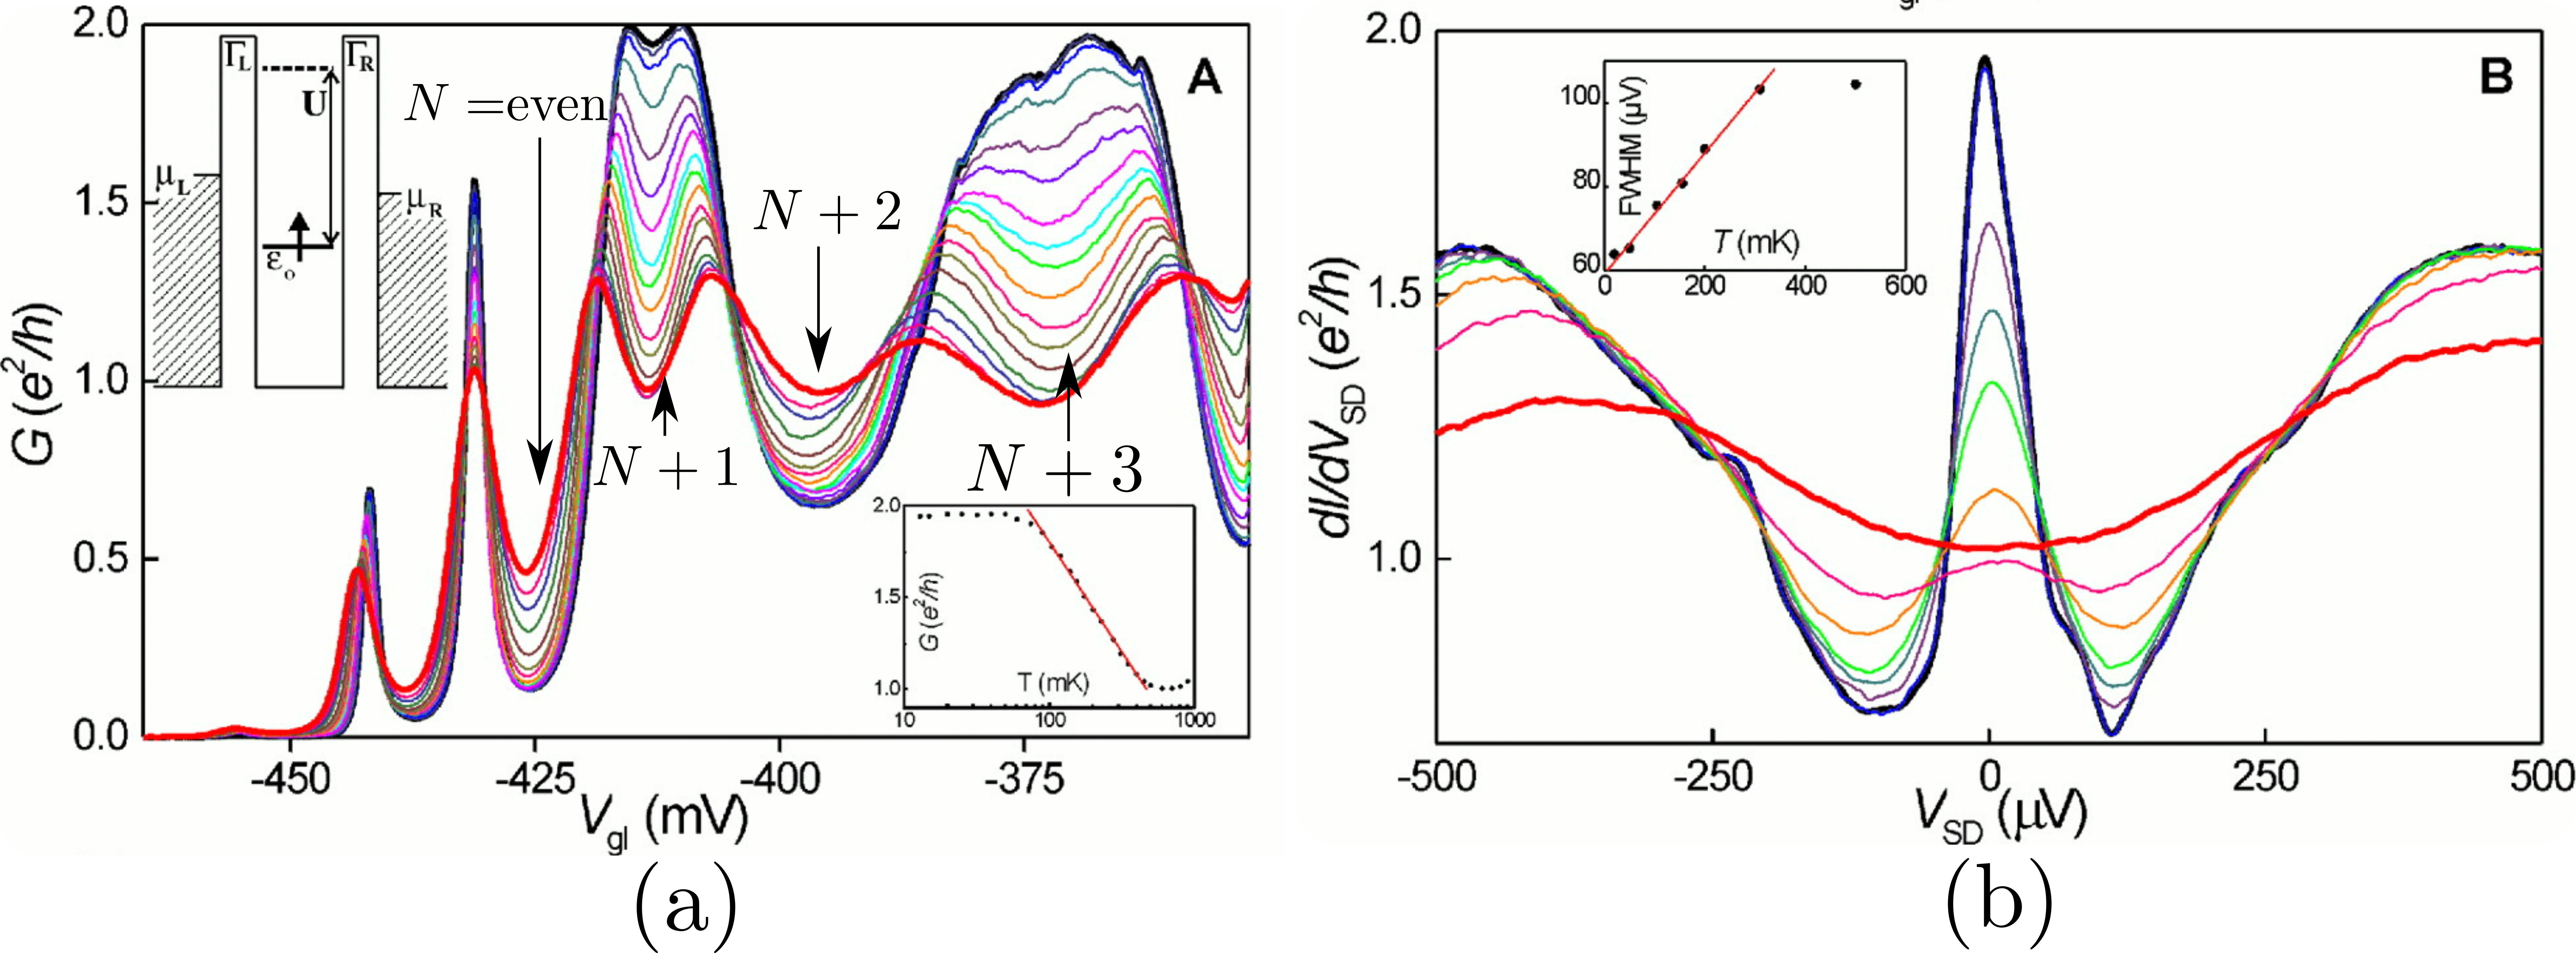
\includegraphics[scale= 0.28]{IMAGES/Preliminars/expKondoQD.png}
  \caption{ \label{fig:ExpKondo} Observation of the Kondo effect in a single electron transistor. Color scale temperatures from 15mk (Black) to 800mk(Red) a) Dependence of the zero bias conductance over the gate voltage. A plateau in the conductance peak appears in the odd particle regimes. b) Dependence of the conductance over the gate source drain voltage inside an odd electron regime. A zero bias conductance peak (ZBCP)  of height $\frac{2e^2}{\hbar}$ is observed. This is the Kondo signature.  \protect\Source{Adapted from \cite{wiel_kondo_2000}}}
\end{figure}


  The problem of magnetic impurities in metals can be treated using the Anderson model in a similar form as the transport in quantum dots. Hence, it is not a surprise that the Kondo Effect could also occur these systems. In 1998 the technological advances allowed the observation of the Kondo effect for the first time in a single electro transistor \cite{goldhaber-gordon_kondo_1998}. When an odd number of electrons is in the QD the last level bellow the Fermi energy is half-occupied, so that the dot can be considered as a magnetic impurity. The unlocalized electrons in the reservoirs then interact with this localized electron. Spin-exchange can occur as it happened with  magnetic impurities in metals. At low temperatures, this magnetic  interaction gives rise to strong quantum correlations that favor the formation of a singlet state between the localized electron and the electrons in the leads. As a result, the zero-bias density of states is increased producing a zero-bias conductance peak \ref{fig:ExpKondo}(b). 

Note that the physical implications of the Kondo effect  are different in magnetic impurities in metals and in QDs. In fact, they are complete opposite. While in magnetic impurities the resistivity increase, the Kondo effect in QD's leads no an unexpected raised in the zero-bias conductivity. The reason for this disagreement between both situations are the are the system dimensions. The scattering against a Kondo singlet in a  $3$D or $2$D systems against magnetic impurities is an obstacle to the conducting electrons. Instead, scattering in 1D-devices enhances the conductivity of the QD because there is only one scattering direction.

 As we previously discussed in \ref{sec:trans}, zero-bias transport in quantum dots can only occur if there is a state at the Fermi energy.  The Kondo effect creates a zero bias peak that is present whenever the dot has odd electrons . This explains the zero-bias plateaus observed in \ref{fig:ExpKondo}(a). We may think that the new singlet at the Fermi energy is creating a "channel" that allows quantum transport between both sides of the dot. This explains the Kondo peak. 

 In the following chapters we will give more details about this zero-energy-mode and theory that  explained it: The numerical renormalization group.  
















% The next part of thess preliminaries will be to compute the conductivity
% through the QD as a function of the gate voltage.
% In regular metals the Kondo effect manifests as a drop in conductivity
% under a certain Kondo temperature $(T_{Kondo})$ due to spin- scattering
% between the conduction electrons and the impurities of the material.
% The Anderson models, hence the NRG, are the perfect tools to study
% the physics of impurieties. Thus the computations we previously developed
% in this chapter will provide the right formalism to introduce the
% Kondo physics. This study will be an important part of the prelimiraries
% in the final document. 



%-----------------------------------------------------------


\chapter{Theory and Methods \label{chap: Methods}}

\section{Ballistic transport \label{sec:transport} }

The Green function $G$ of a Hamiltonian $H$ is the operator that satisfies the homogenous equation 
\begin{equation}
    \left(i\hbar\frac{\partial}{\partial t}-H\right)G\left(t-t'\right)=\delta(t-t').
\end{equation}

This type of differential equations are solved taking the Fourier transform 
\begin{equation}
    \Green{H}=\int_{-\infty}^{\infty}G(t-t')e^{i\omega(t-t')/\hbar}\delta(t-t')
\end{equation}

In this new space the solution of the equation is 
$$(\omega+is -H)\Green{\omega}=I.$$ 

The term $+is$ in the previous hamiltonian is part of a mathematical trick quite common in this theory. During the whole procedure, the Green function acts on the complex field. But when we need to obtain a physical interpretation we will take the limit $s\rightarrow0$ to obtain the result for real energies. 
The next step is to decompose $\Green{H}$ in the eigenbase of the Hamiltonian $\{\ket{\alpha}\}$  by 


\begin{equation}
    \Green{\alpha,\alpha'}=\langle \alpha  \vert \Green{H}\ket{\alpha'}=\frac{\delta_{\alpha\alpha'}}{\omega - is -\ep_\alpha}=\frac{\delta_{\alpha\alpha'}(\omega + is -\ep_\alpha)}{(\omega-\epsilon_{\alpha})^{2}+s^{2}}.
\end{equation}

From the famous formula 
\begin{equation}
\lim_{s\rightarrow0}\frac{s}{(\omega-\epsilon_{\alpha})^{2}+s^{2}}=\pi\delta(\omega-\epsilon_{\alpha})
\end{equation}
we obtain 
\begin{equation}
    Im[\Green{\alpha,\alpha'}] = \pi \delta(\omega -\epsilon_\alpha)\delta_{\alpha,\alpha'}.
\end{equation}
Note that the sum of $Im[\Green{\alpha,\alpha}]$ over all the eigenstates of $H$ is simply the $\pi$ times the Density of States:

\begin{equation}
    \rho(\omega)=-\frac{1}{\pi} Im \left[\Green{\alpha,\alpha}^{\dagger}\right].
\end{equation}

An extended definition of the Green function  can be given in terms of fermionic operators in second quantization.  The time-green function for two fermionic operators $A$ and $B$ is
\begin{equation}
  G_{A,B}(t-t') = \mathcal{T}[\{ A(t),B(t') \} ].
\end{equation}
Here, causality is important, which is the reason why we use the time-order operator $\mathcal{T}$. Again, it is possible to define the green-functions in the energy space applying a Fourier transform. The evolution of these Green functions will be determined by the Schrodringuer equation. At the end, the result will be

\begin{equation}
    \omega\Green{A,B}=\delta_{A^{\dagger},B}+\Green{\left[A,H\right],B}.
\end{equation}

The equation above receives the name of transport equation. This will be our leading method to compute the green functions of the system. In addition we can define the Density of states associated to an operator $A$ to be 

\begin{equation}
    \rho_{A,A^\dagger}=-\frac{1}{\pi}Im\left[\Green{A,A^\dagger}\right].
    \label{eq:Density of States}
\end{equation}

This density of states contains important physical information related to operator $A$. In our case, operator $A^\dagger$ will be related to the creation operator of a quantum dot $d^\dagger$. Our mean purpose will be to compute the density of states of a quantum dot $\rho_{d,d^\dagger}$. This 
that allows us to obtain other transport 

\subsection{Solving transport equations using graphs \label{sec:GraphMethod}}


Solving transport equation involves solving a set of linear equations depending on our energy parameter $\omega$. Though this process can be performed by performed by using current matrix procedures like Gauss-Jordan or even writing the matrix in Mathematica. However, if the model is too complex the solution of the problem will be give a huge equation, difficult to understand. \\

Instead of this we prefer to use graph theory to provide a shortcut to the solution of transport equations. The reason for this is that complex Hamiltonian usually do not  connect all the operators. This means that the total matrix representing the transport equations is full of $0$'a . Graphs allows us to understand these connections, including which operators are connected and which are not,  and then use them to decompose the solution of the green equation.\\ 


To explain the idea behind graph method we will solve the transport equations for a non-interacting $(U=0)$ DQD connected to one lead. According to the Anderson model the Hamiltonian for this system looks like 
\begin{equation}
    H=\epsilon_{di}d_{i}^{\dagger}d_{i}+t_{dots}\left(d_{1}^{\dagger}d_{2}+d_{2}^{\dagger}d_{1}\right)+\sum_{k}\left(V_{i}d_{i}^{\dagger}c_{\mathbf{k}}+V_{i}^{*}c_{\mathbf{k}}^{\dagger}d_{i}\right).
\end{equation} 


with $i$ summing over the terms $\{1,2\}$. Since the system is non-interacting we can ignore the spin-degeneracy in the Hamiltonian. Using we can compute the following  of transport equations for this system.
\begin{align}
     \left(\omega-\epsilon_{1}\right)\Green{d_{1},d_{1}^{\dagger}}&=1+t_{dots}\Green{d_{2},d_{1}^{\dagger}}+V_{1}^{*}\sum_{\mathbf{k}}\Green{c_{\mathbf{k}},d_{1}^{\dagger}} \label{eq:green1}  \\
     \left(\omega-\epsilon_{\mathbf{k}}\right)\Green{c_{\mathbf{k}},d_{1}^{\dagger}} &= V_{1}\Green{d_{1},d_{1}^{\dagger}}+V_{2}\Green{d_{2},d_{1}^{\dagger}} \label{eq:green2} \\
     \left(\omega-\epsilon_{2}\right)\Green{d_{2},d_{1}^{\dagger}}&= t_{dots}\Green{d_{1},d_{1}^{\dagger}}+V_{2}^{*}\sum_{\mathbf{k}}\Green{c_{\mathbf{k}},d_{1}^{\dagger}} \label{eq:green3} 
\end{align}
    %  \left(\omega-\epsilon_{1}\right)\Green{d_{1},d_{1}^{\dagger}}	= & 1+t_{dots}\Green{d_{2},d_{1}^{\dagger}}+V_{1}^{*}\sum_{\mathbf{k}}\Green{c_{\mathbf{k}},d_{1}^{\dagger}} \\

    % \left(\omega-\epsilon_{\mathbf{k}}\right)\Green{c_{\mathbf{k}},d_{1}^{\dagger}}= & V_{1}\Green{d_{1},d_{1}^{\dagger}}+V_{2}\Green{d_{2},d_{1}^{\dagger}} \\

    % \left(\omega-\epsilon_{2}\right)\Green{d_{2},d_{1}^{\dagger}}= & t_{dots}\Green{d_{1},d_{1}^{\dagger}}+V_{2}^{*}\sum_{\mathbf{k}}\Green{c_{\mathbf{k}},d_{1}^{\dagger}}. \\
 Note that we only wrote  the green functions where the second operator is $d_1^\dagger$. This system is already closed which means that we don't need any other equation to find the solution. 

Our objective is to compute the green function for $\Green{d_{1\downarrow},d_{1\downarrow}^{\dagger}}$. This process consist in solving the system of $3$ linear differential equations, which is not difficult.  In fact it is possible to compute the result to be 

\begin{equation}
\Green{d_{1},d_{1}^{\dagger}}=\frac{1}{\left(\omega-\epsilon_{1}-\sum_{\mathbf{k}}\frac{V_{1}V_{1}^{*}}{\omega-\epsilon_{\mathbf{k}}}\right)-\frac{\left(t_{dots}+\sum_{\mathbf{k}}\frac{V_{1}V_{2}^{*}}{\omega-\epsilon_{\mathbf{k}}}\right)\left(t_{dots}+\sum_{\mathbf{k}}\frac{V_{1}V_{2}^{*}}{\omega-\epsilon_{\mathbf{k}}}\right)^{*}}{\omega-\epsilon_{2}-\sum_{\mathbf{k}}\frac{\Gamma_{2}^{2}}{\omega-\epsilon_{\mathbf{k}}}}}. \label{eq:solGreen}
\end{equation}

However this method lacks of any useful intuition that could help us  to  solve more complex systems. This remarks the  importance of pursuing alternative methods. \\

This procedure is what we called the graph method.  We will call our graph $\GDQD$ to imply that it represents a Double Quantum Dot. The vertexes of this graph will be the operator appearing in the left-side of the green functions in  \eqref{eq:green1}\eqref{eq:green2}\eqref{eq:green3}. These  are $d_{1\downarrow},d_{2},c_{\boldsymbol{k}}$. $d_1^\dagger$ is not included since it only appears in the right of the green function. 

We then proceed to define the edges. Let $v_1$ and $v_2$ be two operators in $\GDQD$. If an operator $v_2$ appears in the right side of the transport equation for vertex $v$, the graph will have  a directed edge from $v_2$ to $v_1$. A weight is assign to this edge given by the coefficient of $v_2$ in $v_1$'s transport equation. Note that this relation is reciprocal since the Hamiltonian is hermitian. Hence if there is an arrow from $v_1$ to $v_2$ with weight $t$, then there there will be an opposite arrow from $v_2$ to $v_1$ with weight $t^*$. e.g. In this case, the tree operators  $d_{1\downarrow},d_{2},c_{\boldsymbol{k}}$ are connected. The weights of these connections are observed in \ref{fig:graphDQD}.\\

\begin{figure}[t]
    \centering
    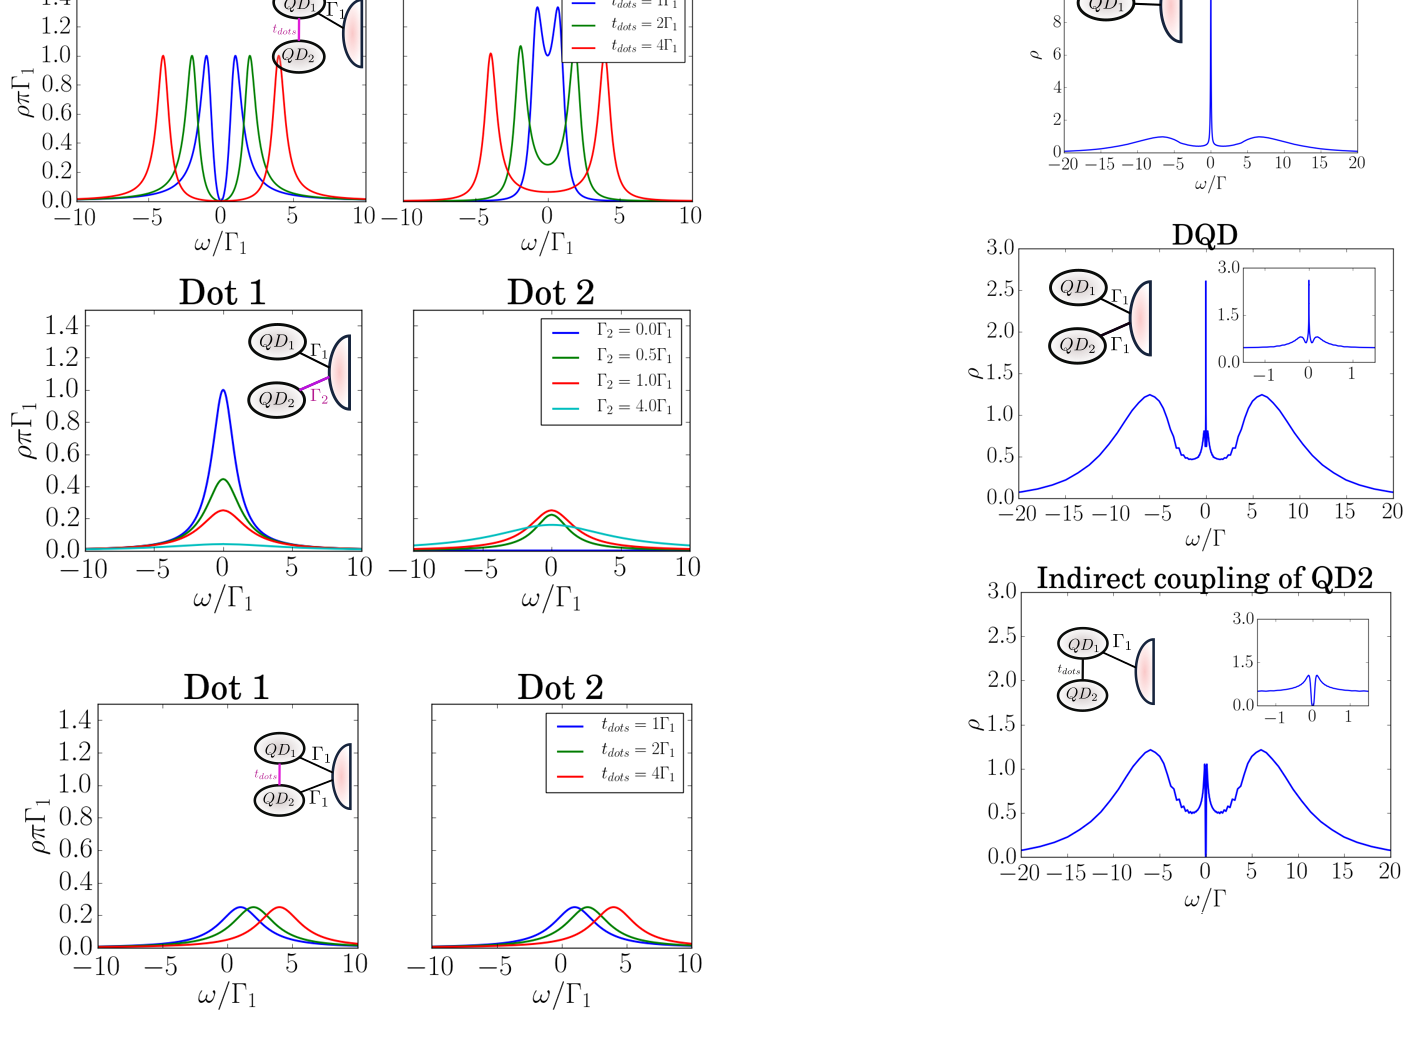
\includegraphics[scale=0.7]{IMAGES/Graphs/DQD.png}
    \caption{ Graph $\GDQD$  \protect\Source{By the author.}}
    \label{fig:graphDQD}
\end{figure}


Now, the Green functions $\Green{d_{1},d_{1}^{\dagger}}$ will always have the form $\frac{1}{\omega-E} $ where $E$ is an energy. This form is also observed in \ref{eq:solGreen}.  Looking at equation \ref{eq:green1},  observe that if $\Green{d_{2},d_{1}^{\dagger}}$ and $\sum_{\mathbf{k}}\Green{c_{\mathbf{k}},d_{1}^{\dagger}}$ are multiples of $\Green{d_{1},d_{1}^{\dagger}}$ (i.e $\Green{d_{2},d_{1}^{\dagger}}=\eta_{2}\Green{d_{1},d_{1}^{\dagger}},\Green{c_{\mathbf{k}},d_{1}^{\dagger}}=\eta_{\boldsymbol{k}}\Green{d_{1},d_{1}^{\dagger}})$ , the result for $\Green{d_{1},d_{1}^{\dagger}}$ will be 
\begin{equation}
    \Green{d_{1},d_{1}^{\dagger}}=\frac{1}{\omega-\epsilon_{1}-\sum_{\boldsymbol{k}}V_{1}^{*}\eta_{\boldsymbol{k}}+t_{dots}\eta_{2}}.
\end{equation}

Hence to obtain $\Green{d_{1},d_{1}^{\dagger}}$ we need to find $\eta_{\boldsymbol{k}}$ and $\eta_{2}$. Now note from equation \eqref{eq:green2} that $\left(\omega-\epsilon_{\boldsymbol{k}}\right)\eta_{\boldsymbol{k}}=V_{1}+V_{2}\eta_{2}$

\begin{equation}
\Green{d_{1},d_{1}^{\dagger}}=\frac{1}{\omega-\epsilon_{1}-\sum_{\boldsymbol{k}}\frac{V_{1}^{*}V_{1}}{\omega-\epsilon_{\boldsymbol{k}}}+V_{1}^{*}V_{2}t_{dots}\eta_{2}\eta_{2}}    
\end{equation}


Now, probably at this point you might already know what is happening here. Basically the energy $E$ represents the sum of all possible transitions in the graph that start and finish at $d_{1}$ . The first term is $\epsilon_{1}$, which is the energy of dot $1$. The next term is $\frac{V_{1}^{*}V_{1}}{\omega-\epsilon_{\boldsymbol{k}}}$ which represents the transition $d_{1}\rightarrow c_{k}\rightarrow d_{1}$. Note that $\frac{V_{1}^{*}V_{1}}{\omega-\epsilon_{\boldsymbol{k}}}$ is basically the energy needed to go from $d_{1}$ to $c_{\boldsymbol{k}}$ and coming back divided by the energy "cost" of passing through $c_{\boldsymbol{k}}$ which is $\omega-\epsilon_{\boldsymbol{k}}$. The sum over $\textbf{k}$ can be ignored in this analysis. Now we can then explain why the last term in \eqref{eq:solGreen} is 
\begin{equation}
    \frac{\left(t_{dots}+\sum_{\mathbf{k}}\frac{V_{1}V_{2}^{*}}{\omega-\epsilon_{\mathbf{k}}}\right)\left(t_{dots}^{*}+\sum_{\mathbf{k}}\frac{V_{1}^{*}V_{2}}{\omega-\epsilon_{\mathbf{k}}}\right)}{\omega-\epsilon_{2}-\sum_{\mathbf{k}}\frac{\Gamma_{2}^{2}}{\omega-\epsilon_{\mathbf{k}}}}. \label{term}
\end{equation}

Firs note that $\left(t_{dots}+\sum_{\mathbf{k}}\frac{V_{1}V_{2}^{*}}{\omega-\epsilon_{\mathbf{k}}}\right)$ is the energy needed to go from $d_{1}$ to $d_{2}$. This could occur by passing through $c_{\boldsymbol{k}} \ \left(\sum_{\mathbf{k}}\frac{V_{1}V_{2}^{*}}{\omega-\epsilon_{\mathbf{k}}}\right)$ or going directly to $d_ 2$ $\left(t_{dots}\right)$. The term is multiplied by $\left(t_{dots}^{*}+\sum_{\mathbf{k}}\frac{V_{1}^{*}V_{2}}{\omega-\epsilon_{\mathbf{k}}}\right)$ which represents the opposed transition from $d_{2}$ to $d_{1}$.  Finally, we  divide this by the cost of passing through $d_{2}$ and $c_{\boldsymbol{k}}$. This is basically to multiply by the green function taking the point $d_{1}$ out of $\GDQD$ . This green function is


\begin{equation}
    \GreenG{d_2,d_2^\dagger}{\GDQD-d1}= \frac{1}{\omega-\epsilon_{2}-\sum_{\mathbf{k}}\frac{\Gamma_{2}^{2}}{\omega-\epsilon_{\mathbf{k}}}}.
\end{equation}
where $\GreenG{d_2,d_2^\dagger}{\GDQD-d_1}$ is the green function of $d_2,d_2^\dagger$ in the smaller graph $\GDQD-d_1$. 

The last equation not only explains the meaning of term \eqref{term} in equation \eqref{eq:solGreen}. It also gives us an iterative method to find the green function. To understand this, note that the solution in \eqref{eq:solGreen} can also be written as 

\begin{equation}
\left( \GreenG{d_{1},d_{1}^{\dagger}}{\GDQD} \right) ^{-1}= \omega - \epsilon_1- \sum_\textbf{k} E_{d_1c_k}^{\GDQD-d_2} \GreenG{c_\textbf{k}c^\dagger_\textbf{k}}{\GDQD-d_2-d_1}  - E_{d_1d_2}^{\GDQD} \GreenG{d_2,d_2^\dagger}{\GDQD-d_1} . \label{eq:solGreen2}
\end{equation}
Where $E_{d_1c_k}^{\GDQD-d_2} = \sum_{\boldsymbol{k}}\frac{V_{1}^{*}V_{1}}{\omega-\epsilon_{\boldsymbol{k}}} $  represents the accumulated energy of going from $d_1$ to $c_k$ and coming back. The upper-index $\GDQD-d_2$ represents that at this step second dot is ignored. Similarly $E_{d_1d_2}^{\GDQD}$ is the numerator of \eqref{term}. It represents the energy accumulated in at going from $d_1$ to $d_2$. Since this time no point is ignored, the upper-index remains as $\GDQD$. \\

Now the amazing thing about the last equation is that it decomposes the green function $\GreenG{d_{1},d_{1}^{\dagger}}{\GDQD}$  into green functions of smaller graphs. This gives an iterative process to compute green functions using induction in graphs .  Now, as you might see, the complexity of these green functions reduce strongly after a single point is removed out of the graph . This makes green function computation a pretty simple task using the graph method. 

\Jesus{I promise a real proof of this fact to be included in the abstract. The idea is using induction in graphs  \ref{sec:AbsGraphmethod}. }

\subsection{Ballistic transport in  Double Quantum Dot \label{sec:GreedDQD}}
The is only one factor missing in equation \eqref{eq:solGreen}. During the  entire procedure we carried the factor $\sum_{\boldsymbol{k}}\frac{V_{1}^{*}V_{1}}{\omega-\epsilon_{\boldsymbol{k}}}$. This factor describes the broadening of the DOS when the QD enters in contact with the lead. This broadening is usually named $\Gamma=V_{1}^{*}V_{1}$ (Or $\Delta$ depending on the text book). 
% $$-\Gamma_i = \sum_{\boldsymbol{k}}\frac{V_{1}^{*}V_{1}}{\omega-\epsilon_{\boldsymbol{k}}}. $$
In general $V_i$  is a function of $\textbf{k}$. However, in the limit of flat-band that is the case we are interested in , we can assume that $V_i $ is constant. Therefore, it is enough to integrate
\begin{equation}
    \sum_{\boldsymbol{k}}\frac{1}{\omega-\epsilon_{\boldsymbol{k}}+is}=\int_{-D}^{D}\frac{d\epsilon_{\boldsymbol{k}}}{\omega-\epsilon_{\boldsymbol{k}}+is}=-\ln\left(\frac{D-\epsilon_{\boldsymbol{k}}+is}{-D-\epsilon_{\boldsymbol{k}}+is}\right)\xrightarrow[D\rightarrow\infty]{}-i.
\end{equation}
Where we assumed that there is a maximum  energy cutoff $D$ going to infinity in the wide-band limit. Hence 
\begin{equation}
   -i\Gamma_i = \sum_{\boldsymbol{k}}\frac{V_{1}^{*}V_{1}}{\omega-\epsilon_{\boldsymbol{k}}}.
\end{equation}

We can replace this in equation \eqref{eq:solGreen} to obtain the real expression for the green function $\Green{d_1,d_1^\dagger}$. The terms of the form $V_1V_2*$ can be replaced for $\sqrt{\Gamma_1\Gamma_2}$, supposing there is no additional complex phase.

Now, remember from \eqref{eq:Density of States} that the DOS $\rho$ depends on the imaginary factor of the Green Function $\Green{d_1,d_1^\dagger}$. This factor is express in the broadening $\Gamma$. In case $\Gamma = 0$ the density of states will be null. At any other case, one of the dots should be attached to the lead. Let $\Gamma_1$ be the broadening of this dot. We will take $\Gamma_1$ as unit.  
In \ref{fig:GreenDQD} we can observe the evolution of the Density of States under certain processes. Each plot includes an inset showing the model applied to the figure. The coupling in purple indicates the tuning variable. In addition, we set $e_1 = e_2 = 0$ so that both dots satisfy hole symmetric 


\begin{enumerate}
    \item \textbf{Coupling QD2 (Figure \ref{fig:DQD-G2}):} It shows the evolution of the DOS when the second dot's coupling scales from $0$ to $4\Gamma$. At $\Gamma_2=0$  the second dot is decoupled. The first dot's DOS is the same of a single dot case. The maximum height is achieved at $\rho \pi \Gamma_1 =1$ and the width at the half of this height $(\rho \pi \Gamma_1 =0.5)$ is $\Gamma_1$ just as in Figure \ref{fig:specDots}. When the second dot is attached $\Gamma_2 >0$ the density of states is divided between both dots. At $\Gamma_1 = \Gamma_2$ both DOS are equal to $\frac{1}{4\pi\Gamma}$. 
    \item \textbf{Indirect Coupling of QD2 (Figure \ref{fig:DQD-tdots}):} This is the most interesting case. When the second dot is connected indirectly through the first dot there appears a quantum inference that splits the central peak in two new states. We will observe later that in the interacting case this procedure can also destroy the Kondo signature. This has interesting consequences when combined with majorana physics, since the interference patter destroy the Kondo effect but not the majorana signature. 
    \item \textbf{Breaking Particle Hole Symmetry (Figure \ref{fig:DQD-PHS}):}
    Suppose we have $\Gamma_2 = \Gamma_1$. The "triangular connections" break Particle Hole Symmetry. The central peak is displaced to the positive part of the spectrum. Contrary to the previous case, this situation will be avoided during this project. This is because breaking PHS in both dots will prevent the Majorana to tunnel inside the DQD. 
    
\end{enumerate}

\newpage
\begin{figure}[H]
     \centering
    
     \subfloat[Attaching QD2 to the lead \label{fig:DQD-G2}]{\includegraphics[scale=0.6]{IMAGES/DQD/g1g2-m.png}} \\
    \subfloat[Indirect connection of QD2 \label{fig:DQD-tdots}]{\includegraphics[scale=0.6]{IMAGES/DQD/tdots-m.png}}\\
    \subfloat[Breaking PHS with triangular connection \label{fig:DQD-PHS}]{\includegraphics[scale=0.6]{IMAGES/DQD/phs-m.png}}
     \caption{\label{fig:GreenDQD} For the tree cases we considered $e_1 =e_2 =0$. The inset shows the set-up. At each case the purple coupling shows the tuning variable. \protect\Source{ By the Author  }}
\end{figure}

\newpage












% --------------------------------------------------
\section{The Numerical Renormalization Group\label{sec:The-Numerical-Renormaliztion} (NRG) }

 
\Jesus{I need to reference Kondo equations. Include advantages}

At low energies a renormalization group approach is necessary to deal with the effects of high correlations. This implies that the divergent resistivity in Kondo model will be renormalized to a finite quantity. 
 


In the 1970's G.Wilson created a numerical method to solve the Anderson model . This method receives the name of Numerical Renormalization Group (NRG) \citep{bulla_numerical_2008,wilson_renormalization_1975,krishna-murthy_renormalization-group_1980}. It consists of three basic steps :
\begin{enumerate}
\item To perform a numerical discretization of the energy spectrum in logarithmic intervals. 
\item To map the discretized model onto a semi-infinity chain Hamiltonian. 
\item  To diagonalize iteratively the chain hamiltonian . 
\end{enumerate}

The final result will be the spectrum of the Hamiltonian. Other important properties of the material such as density of states, conductivity, specific heat, susceptibility can also be computed. On this project we are mainly interested in the Density of States (DOS). The method used to compute the DOS is the Density Matrix numerical renormalization Group (DM-NRG). A complete description of this algorithm will be given in the followin sections.  \\

For now, we proceed to describe how the NRG is applied to solve the Anderson model in a QD:\\

\Jesus{I still need to do a long revision to this section. Probably I will send most of the computations to the abstract and leave a summary of NRG and its advantages in the main text.}

\subsubsection{Logarithmic Discretization:}



We start with an Anderson model hamiltonian such as the one 
in \prettyref{eq:Anderson} without magnetic field

\begin{equation}
H=\frac{U}{2}+\sum_{\sigma}\left[\left(\epsilon_{d}+\frac{U}{2}\right)d_{\sigma}^{\dagger}d_{\sigma}+\frac{U}{2}(d_{\sigma}^{\dagger}d_{\sigma}-1)^{2}+\sum_{\mathbf{k}}\ep_{\mathbf{k}}c_{\mathbf{k}\sigma}^{\dagger}c_{\mathbf{k}\sigma}+V_{\mathbf{k}}d_{\sigma}^{\dagger}c_{\mathbf{k}\sigma}+V_{\mathbf{k}}^{*}c_{\mathbf{k}\sigma}^{\dagger}d_{\sigma}\right].\label{HamWilson}
\end{equation}

At low-energies we can assume that QD couples only to s-wave states in the leads\citep{krishna-murthy_renormalization-group_1980}. This implies that that the Fermi surface is contained
in a single, isotropic conduction band extending inside some fixed cutoffs $-D$ and $D$. Thus, $\epsilon_{\mathbf{k}}$ only depends on $\left|\mathbf{k}\right|$. This makes possible to transform the sum over $\mathbf{k}$ in
equation \ref{HamWilson} into an integral over $\epsilon$ between
the energy cutoffs
\begin{eqnarray}
H & =\sum_{\sigma} & \Biggl[\left(\epsilon_{d}+\frac{U}{2}\right)d_{\sigma}^{\dagger}d_{\sigma}+\frac{U}{2}(d_{\sigma}^{\dagger}d_{\sigma}-1)^{2}+\int_{-D}^{D}\mbox{d}\epsilon\ \epsilon c_{\epsilon\sigma}^{\dagger}c_{\epsilon\sigma}\nonumber \\
 &  & \qquad\qquad\qquad\qquad\qquad\qquad+\int_{-D}^{D}\sqrt{\rho_{\sigma}(\epsilon)}\mbox{d}\epsilon\ V_{\epsilon}d_{\sigma}^{\dagger}c_{\mathbf{k}\sigma}+V_{\epsilon}^{*}c_{\epsilon\sigma}^{\dagger}d_{\sigma}\Biggr].\label{eq:hamEnergy}
\end{eqnarray}


Here $c_{\epsilon\sigma}^{\dagger}$ creates an electron with energy
$\epsilon$ and $\rho_{\sigma}(\epsilon)$ is the density of states
of the system per spin, which appears in the integral due to the change
of variable from $\mathbf{k}$ to $\epsilon\propto\left|\mathbf{k}\right|^{2}.$
Finally, we ignore the energy dependence of $\rho$ and $V_{d}$ and
we replace them by their values in the Fermi energy (This approximation
has no great relevance which is justified in \citep{krishna-murthy_renormalization-group_1980})
and we renormalize the energy band doing the replacements $k=\frac{\epsilon}{D}$
and $c_{k\sigma}:=\sqrt{D}c_{\epsilon\sigma}$ so that \prettyref{eq:hamEnergy}
becomes

\begin{eqnarray}
H & = & D\sum_{\sigma}\Biggl[\frac{1}{D}\left(\epsilon_{d}+\frac{U}{2}\right)d_{\sigma}^{\dagger}d_{\sigma}+\frac{U}{2D}(d_{\sigma}^{\dagger}d_{\sigma}-1)^{2}+\int_{-1}^{1}\mbox{d}k\ kc_{k\sigma}^{\dagger}c_{k\sigma}\nonumber \\
 &  & \qquad\qquad\qquad\qquad\qquad\qquad\qquad+\sqrt{\frac{\Gamma}{\pi D}}\int_{-1}^{1}\mbox{d}k\ d_{\sigma}^{\dagger}c_{k\sigma}+c_{k\sigma}^{\dagger}d_{\sigma}\label{eq:Norm-HamEnergy}\\
 & = & H_{d}+D\sum_{\sigma}\Biggl[\int_{-1}^{1}\mbox{d}k\ kc_{k\sigma}^{\dagger}c_{k\sigma}+\sqrt{\frac{\Gamma}{\pi D}}\int_{-1}^{1}\mbox{d}k\ d_{\sigma}^{\dagger}c_{k\sigma}+c_{k\sigma}^{\dagger}d_{\sigma}\Biggr],
\end{eqnarray}


\begin{figure}[h]
\centering
\includegraphics[scale=0.3]{IMAGES/Log-disc.png}\caption{\label{FigDiscretization} Taken from \citep{krishna-murthy_renormalization-group_1980}.
Energy interval discretization. \label{Energy-interval-discretization}}
\end{figure}


where $\Gamma=\pi\rho V^{2}$ is associated to the lever-width \citep[(3.5)]{sindel_numerical_2005}.
At this point we have our model dependent of three unit-less constants
$\frac{\epsilon_{d}}{D}\ ,\ \frac{U}{2D}$ and $\frac{\Gamma}{\pi D}$.
The logarithmic discretization starts by defining an scaling parameter
$\Lambda\geq1$ in diving the energy domain $[-1,1]$ into an array
of intervals of the form $\{[\pm\Lambda^{-(n+1)},\pm\Lambda^{n}]\}_{n\in\mathbb{N}}$,
as we can observe in \ref{FigDiscretization}. Note that the width
of these intervals is decreasing exponentially by 
\[
d_{n}=\Lambda^{-n}\left(1-\Lambda^{-1}\right).
\]


Then inside of these energy intervals we can define a set of orthonormal
Fourier series of the form
\begin{equation}
\phi_{np}^{\pm}(\epsilon)=\begin{cases}
\frac{1}{\sqrt{d_{n}}}e^{\pm i\omega_{n}p\epsilon} & \epsilon\in[\pm\Lambda^{-(n+1)},\pm\Lambda^{n}]\\
0 & \mbox{a.o.c },
\end{cases}\label{eq:orthonormal-Fourier}
\end{equation}


with $\omega_{n}:=\frac{2\pi}{d_{n}}$ so that $\phi_{np}^{\pm}\left(\pm\Lambda^{-(n+1)}\right)=\phi_{np}^{\pm}\left(\pm\Lambda^{-n)}\right).$
Then we can decompose the creation operators $c_{k}^{\dagger}$ into
their interval-Fourier contributions as 
\begin{equation}
c_{k\sigma}^{\dagger}=\sum_{np}\phi_{np}^{+}(k)c_{np\sigma}^{+\dagger}+\phi_{np}^{-}(k)c_{np\sigma}^{-\dagger}\label{eq:Fourier-interval decomposition}
\end{equation}


with the new creation operators defined as 
\[
c_{np\sigma}^{\pm\dagger}:=\left(c_{np\sigma}^{\pm}\right)^{\dagger}=\int_{-1}^{1}\mbox{d}\epsilon\ \left[\phi_{np}^{+}(\epsilon)\right]^{*}c_{\epsilon\sigma}^{\dagger}.
\]


This decomposition \prettyref{eq:Fourier-interval decomposition}
is a simple consequence of the orthonormality of the functions defined
in \prettyref{eq:orthonormal-Fourier}. In addition we can readily
proof that $c_{np\sigma}^{\pm\dagger}$-operators satisfy the anti-commutation
relations, so that they are rightful fermionic creation operators. 

We can now use \prettyref{eq:Fourier-interval decomposition} to replace
the $k$-dependent terms in hamiltonian \prettyref{eq:Norm-HamEnergy}.
Then we obtain

\begin{eqnarray}
\int_{-1}^{1}\mbox{d}k\ c_{k\sigma}^{\dagger}d_{\sigma} & = & \int_{-1}^{1}\mbox{d}k\ \left(\sum_{np}\phi_{np}^{+}(k)c_{np\sigma}^{+\dagger}+\phi_{np}^{-}(k)c_{np\sigma}^{-\dagger}\right)d_{\sigma}\nonumber \\
 & = & \left(\sum_{np}\left(\int_{-1}^{1}\mbox{d}k\ \phi_{np}^{+}(k)\right)c_{np\sigma}^{+\dagger}+\left(\int_{-1}^{1}\mbox{d}k\ \phi_{np}^{-}(k)\right)c_{np\sigma}^{-\dagger}\right)d_{\sigma}\nonumber \\
 & = & \left(\sum_{np}\left(\int_{\Lambda^{-(n+1)}}^{\Lambda^{-n}}\mbox{d}k\ \frac{e^{i\omega_{n}pk}}{\sqrt{d_{n}}}\right)c_{np\sigma}^{+\dagger}+\left(\int_{-\Lambda^{-n}}^{-\Lambda^{-(n+1)}}\mbox{d}k\ \frac{e^{-i\omega_{n}pk}}{\sqrt{d_{n}}}\right)c_{np\sigma}^{-\dagger}\right)d_{\sigma}\nonumber \\
 & = & \left(\sum_{np}\sqrt{d_{n}}\delta_{p}c_{np\sigma}^{+\dagger}+\sqrt{d_{n}}\delta_{p}c_{np\sigma}^{-\dagger}\right)d_{\sigma}\nonumber \\
 & = & \sqrt{1-\Lambda^{-1}}\sum_{n}\Lambda^{-\frac{n}{2}}\left(c_{np\sigma}^{+\dagger}+c_{np\sigma}^{-\dagger}\right)d_{\sigma}.\label{eq:firt-Integral}
\end{eqnarray}


And 

\begin{eqnarray}
\int_{-1}^{1}\mbox{d}k\ kc_{k\sigma}^{\dagger}c_{k\sigma} & = & \sum_{n,n',p,p'}\sum_{s,s'=\pm}\left(\int_{-1}^{1}k\mbox{d}k\ \phi_{np}^{s}(k)\left(\phi_{np}^{s'}(k)\right)^{*}\right)c_{np\sigma}^{s\dagger}c_{n'p'\sigma}^{s'}\nonumber \\
 & = & \sum_{n,n',p,p'}\sum_{s,s'=\pm}\left(\frac{\delta_{nn'}\delta_{ss'}}{d_{n}}\int_{\Lambda^{-(n+1)}}^{\Lambda^{-n}}k\mbox{d}k\ e^{is\omega_{n}k\left(p-p'\right)}\right)c_{np\sigma}^{s\dagger}c_{np'\sigma}^{s}\nonumber \\
 & = & \sum_{npp'}\sum_{s=\pm}\left(\frac{s}{2}\Lambda^{-2n}\left(1-\Lambda^{-2}\right)\delta_{pp'}+\frac{1-\delta_{pp'}}{is\omega_{n}\left(p-p'\right)}\left[ke^{is\omega_{n}k\left(p-p'\right)}\right]_{\Lambda^{-(n+1)}}^{\Lambda^{-n}}\right)\frac{c_{np\sigma}^{s\dagger}c_{np'\sigma}^{s'}}{d_{n}}\nonumber \\
 & = & \frac{1}{2}\left(1+\Lambda^{-1}\right)\sum_{np}\Lambda^{-n}\left(c_{np\sigma}^{+\dagger}c_{np\sigma}^{+}-c_{np\sigma}^{-\dagger}c_{np\sigma}^{-}\right)\nonumber \\
 &  & \ \ \ \ \ \ \!\ \ \ \ \!\ \ +\sum_{n}\sum_{p\neq p'}\frac{1-\Lambda^{-1}}{2i\pi\left(p'-p\right)}\left(c_{np\sigma}^{+\dagger}c_{np'\sigma}^{+}-c_{np'\sigma}^{-\dagger}c_{np\sigma}^{-}\right)e^{\frac{2i\pi\left(p-p'\right)}{1-\Lambda^{-1}}}.\label{eq:second-integral}
\end{eqnarray}


Thus, if we replace \prettyref{eq:firt-Integral} and \prettyref{eq:second-integral}
into \prettyref{eq:Norm-HamEnergy} we will obtain a logarithmic discretization
of the hamiltonian. The next part will we to map this discretization
to an iterative process that is worth for a numerical computations. 

\subsubsection{Mapping the Anderson model to a Chain-Hamiltonian}

\begin{figure}[h]
\centering
\includegraphics[scale=0.5]{IMAGES/NRGchain.png}\caption{\label{FigNRG-chain} Chain-Hamiltonian describing the Anderson model.
The chain starts at the initial dot hamiltonian $H_{d}$. The $f_{m}^{\dagger}$'s
are the creation operators at the $n^{\mbox{th}}$-site of the chain.
The $\xi_{n}$'s describe the magnitude of the interaction between
consecutive sites. }
\end{figure}


We are looking for a model just like the one we have in \ref{FigNRG-chain}.
This is because a Chain-Hamiltonian will give an iterative approximation
of the Anderson model with an increasing (but still controllable)
number of degrees of freedom. This will provide the rightful structure
for a numerical diagonalization of the hamiltonian. \\

To do this, observe from equations \prettyref{eq:firt-Integral},\prettyref{eq:second-integral}
that the QD ($d_{\sigma}$) couples directly only to the operators
with $p=0$$\left(c_{n0\sigma}^{\pm\dagger}\right)$. The $p\neq0$
terms will appear in the hamiltonian only because they are coupled
to $c_{np\sigma}^{+\dagger}$ in Equation \prettyref{eq:second-integral}.
Thus, as a first approximation we can neglect all terms in \prettyref{eq:second-integral}
with $p\neq0$. This leaves only the first part of \prettyref{eq:second-integral},
so that we can define $c_{n\sigma}^{\pm\dagger}:=c_{np\sigma}^{\pm\dagger}$
. Let 
\begin{equation}
f_{0\sigma}^{\dagger}=\sqrt{\frac{1-\Lambda^{-1}}{2}}\sum_{n}\Lambda^{-\frac{n}{2}}\left(c_{n\sigma}^{+\dagger}+c_{n\sigma}^{-\dagger}\right),\mbox{ so that }\sqrt{2}f_{0\sigma}^{\dagger}d_{\sigma}=\int_{-1}^{1}\mbox{d}k\ c_{k\sigma}^{\dagger}d_{\sigma}.\label{eq:f_0}
\end{equation}


Note $\left\{ f_{0\sigma}^{\dagger},f_{0\sigma}\right\} =\frac{1-\Lambda^{-1}}{2}\sum_{n}2\Lambda^{-n}=1$.
Replacing this in \prettyref{eq:Norm-HamEnergy}we get 
\[
H=H_{d}+D\sum_{\sigma}\Biggl[\sqrt{\frac{2\Gamma}{\pi D}}\left(d_{\sigma}^{\dagger}f_{0\sigma}+f_{0\sigma}^{\dagger}d_{\sigma}\right)+\frac{1}{2}\left(1+\Lambda^{-1}\right)\sum_{n}\Lambda^{-n}\left(c_{n\sigma}^{+\dagger}c_{n\sigma}^{+}-c_{n\sigma}^{-\dagger}c_{n\sigma}^{-}\right)\Biggr].
\]


$f_{0}^{\dagger}$will represent the first site of the chain-hamiltonian
in \ref{FigNRG-chain} since no other term is coupled to the dot hamiltonian.
We also have the coupling term $\xi_{0}=\sqrt{\frac{2\Gamma}{\pi D}}$.
It is possible to obtain the following $f_{m}^{\dagger}$-operators
by supposing a solution of the form 
\begin{equation}
f_{m\sigma}^{\dagger}=\sum_{n}a_{mn}^{+}c_{n\sigma}^{+\dagger}+a_{mn}^{-}c_{n\sigma}^{-\dagger}=\sum_{n}\sum_{s=\pm}a_{mn}^{s}c_{n\sigma}^{s\dagger},\label{eq:chain elements}
\end{equation}
 such that they satisfy the anti-commutation relations 
\[
\left\{ f_{m\sigma}^{\dagger},f_{m\sigma}\right\} =\delta_{mm'}\delta_{\sigma\sigma'}\ ,\ \left\{ f_{m\sigma}^{\dagger},f_{m\sigma}^{\dagger}\right\} =\left\{ f_{m\sigma}^{\dagger},f_{m\sigma}^{\dagger}\right\} =0
\]
and 
\begin{equation}
\frac{1}{2}\left(1+\Lambda^{-1}\right)\sum_{n}\Lambda^{-n}\left(c_{n\sigma}^{+\dagger}c_{n\sigma}^{+}-c_{n\sigma}^{-\dagger}c_{n\sigma}^{-}\right)=\sum_{m=0}^{\infty}\Lambda^{\frac{-m}{2}}\xi_{m}\left(f_{m\sigma}^{\dagger}f_{m+1,\sigma}+f_{m+1\sigma}^{\dagger}f_{m\sigma}\right).\label{eq:final equation}
\end{equation}


It is possible to find a solution for this system using the formula of
the right part of equation \ref{eq:final equation}. Since the relation
is only given between consecutive terms $m,m+1$ and we already have
the coefficients for $m=0$ $\left(a_{0n}^{s}=\sqrt{\frac{1-\Lambda^{-1}}{2}}\Lambda^{-\frac{n}{2}}\right).$
Then it is possible to determine the upper coefficients in a recursive way starting
from $m=0$. Supposing we can obtain the $m^{\mbox{th}}$-coefficients
$(a_{mn}^{s})$ and then finding iteratively the coefficients of $m+1\ (a_{mn}^{s})$
using the relation given by equation \prettyref{eq:final equation}.
This provides a numerical way for obtaining the $f_{m\sigma}^{\dagger}$
operators. In fact in our case, where we actually did important assumptions,
the problem can be solved analytically obtaining that the final hamiltonian
is given by 

\begin{equation}
H=H_{d}+D\sum_{\sigma}\Biggl[\sqrt{\frac{2\Gamma}{\pi D}}\left(d_{\sigma}^{\dagger}f_{0\sigma}+f_{0\sigma}^{\dagger}d_{\sigma}\right)+\frac{1}{2}\left(1+\Lambda^{-1}\right)\sum_{n=0}^{\infty}\Lambda^{\frac{-n}{2}}\xi_{n}\left(f_{n\sigma}^{\dagger}f_{n+1,\sigma}+f_{n+1\sigma}^{\dagger}f_{n\sigma}\right)\Biggr].\label{eq:chain-Hamiltonian}
\end{equation}


with 
\[
\xi_{n}=\frac{1-\Lambda^{-n-1}}{\left(1-\Lambda^{-2n-1}\right)^{\frac{1}{2}}\left(1-\Lambda^{-2n-3}\right)^{\frac{1}{2}}}.
\]


The formal recursive-solution of this problem can be found in \citep{bulla_numerical_2008}
. Note that equation \prettyref{eq:chain-Hamiltonian} describes the
chain hamiltonian model that we where looking for in \ref{FigNRG-chain}.
Note that in the limit when $n\longrightarrow\infty$ 

\[
\Lambda^{\frac{-n}{2}}\xi_{n}\longrightarrow\frac{\Lambda^{\frac{-n}{2}}\left(1-\Lambda^{-n}\right)}{1-\Lambda^{-2n}}\sim\frac{\Lambda^{\frac{-n}{2}}}{1+\Lambda^{-n}},
\]


which implies an exponential decaying of the hopping term in the chain. 

\subsubsection{Iterative Diagonalization in a Single QD process}

Now that we have an iterative representation of the Anderson Model
Hamiltonian \prettyref{eq:chain-Hamiltonian}, lets take a look to
how the NRG code would work for a QD. We start with the dot hamiltonian.
(Since the $D$ term is always present as a normalizing factor, we
are going to avoid this term in future computations and suppose that
we are working with unit-less variables $\epsilon_{d},\ U$ and $\Gamma':=\sqrt{\frac{2\Gamma}{\pi D}}$
).
\begin{equation}
H_{d}=\frac{1}{D}\left(\epsilon_{d}+\frac{U}{2}\right)d_{\sigma}^{\dagger}d_{\sigma}+\frac{U}{2D}(d_{\sigma}^{\dagger}d_{\sigma}-1)^{2}.\label{eq:DotHam}
\end{equation}


Now observe that hamiltonian \ref{eq:DotHam} already has a
diagonal form in the base $\left\{ \vert\uparrow\!\downarrow\rangle,\vert\uparrow\rangle,\vert\downarrow\rangle,\vert0\rangle\right\} $
\[
H_{d}=\frac{1}{D}\left[\begin{array}{cccc}
2\epsilon_{d}+\frac{3U}{2} & 0 & 0 & 0\\
0 & \epsilon_{d}+\frac{U}{2} & 0 & 0\\
0 & 0 & \epsilon_{d}+\frac{U}{2} & 0\\
0 & 0 & 0 & \frac{U}{2}
\end{array}\right].
\]


Lets define $H_{-1}=\Lambda^{\frac{-1}{2}}H_{d}.$ Adding the first
chain interaction to $H_{d}$ we obtain a new hamiltonian of the form 

\begin{equation}
H_{0}=\Lambda^{\frac{1}{2}}H_{-1}+\Gamma'\left(d_{\sigma}^{\dagger}f_{0\sigma}+f_{0\sigma}^{\dagger}d_{\sigma}\right).\label{eq:H0fromH-1}
\end{equation}


The Hilbert space for this hamiltonian has to be extended to include
the $4$ degrees of freedom of the $f_{0\sigma}^{\dagger}$ particles
which are also given by $\left\{ \vert\uparrow\!\downarrow\rangle,\vert\uparrow\rangle,\vert\downarrow\rangle,\vert0\rangle\right\} $.
Therefore the total Hilbert space for $H_{0}$ is given by a base
of the form 
\[
\vert s_{1}\rangle\vert s_{2}\rangle:=\vert s_{1}\rangle\otimes\vert s_{2}\rangle\mbox{ with }\vert s_{1,2}\rangle\in\left\{ \vert\uparrow\!\downarrow\rangle,\vert\uparrow\rangle,\vert\downarrow\rangle,\vert0\rangle\right\} .
\]


This gives an space of dimension $4\times4=16.$ Now before adventuring
to write the hamiltonian for $H_{0}$ as a $16\times16$-matrix note
that $H_{0}$ preserves particle number $N$ and the total spin $S$.
 Therefore we can use  $N$ and $S$ as quantum numbers and generate the Hamiltonian $H_{0}$ in blocks.
We will observe that the terms in the diagonal will correspond to
the eigenvalues of $H_{-1}$ for the first space. The non-diagonal
terms are the result of the hopping interactions with the first site. 

\begin{multicols}{2}

$H_{N=0,S=0}:$
\[
\begin{array}{c}
\vert0\rangle\vert0\rangle\rightarrow\end{array}\begin{array}{c}
\left[\frac{U}{2}\right]\end{array}
\]


$H_{N=4,S=0}:$
\[
\begin{array}{c}
\vert\uparrow\!\downarrow\rangle\vert\uparrow\!\downarrow\rangle\rightarrow\end{array}\begin{array}{c}
\left[2\epsilon_{d}+\frac{3U}{2}\right]\end{array}
\]


\end{multicols}

\begin{multicols}{2}

$H_{N=1,S=\frac{1}{2}}:$
\[
\begin{array}{c}
\vert\uparrow\rangle\vert0\rangle\rightarrow\\
\vert0\rangle\vert\uparrow\rangle\rightarrow
\end{array}\left[\begin{array}{cc}
\epsilon_{d}+\frac{U}{2} & \Gamma'\\
\Gamma' & \frac{U}{2}
\end{array}\right]
\]


$H_{N=1,S=\frac{-1}{2}}:$
\[
\begin{array}{c}
\vert\uparrow\rangle\vert0\rangle\rightarrow\\
\vert0\rangle\vert\uparrow\rangle\rightarrow
\end{array}\left[\begin{array}{cc}
\epsilon_{d}+\frac{U}{2} & \Gamma'\\
\Gamma' & \frac{U}{2}
\end{array}\right]
\]


\end{multicols}

\begin{multicols}{2}

$H_{N=2,S=-1}:$
\[
\begin{array}{c}
\vert\downarrow\rangle\vert\downarrow\rangle\rightarrow\end{array}\begin{array}{c}
\left[\epsilon_{d}+\frac{U}{2}\right]\end{array}
\]


$H_{N=2,S=1}:$
\[
\begin{array}{c}
\vert\uparrow\rangle\vert\uparrow\rangle\rightarrow\end{array}\begin{array}{c}
\left[\epsilon_{d}+\frac{U}{2}\right]\end{array}
\]


\end{multicols}
\begin{figure}[t]
\subfloat[$N$ takes only even values]{\includegraphics[scale=0.5]{IMAGES/even.png}}\subfloat[$N$ run only through odd values]{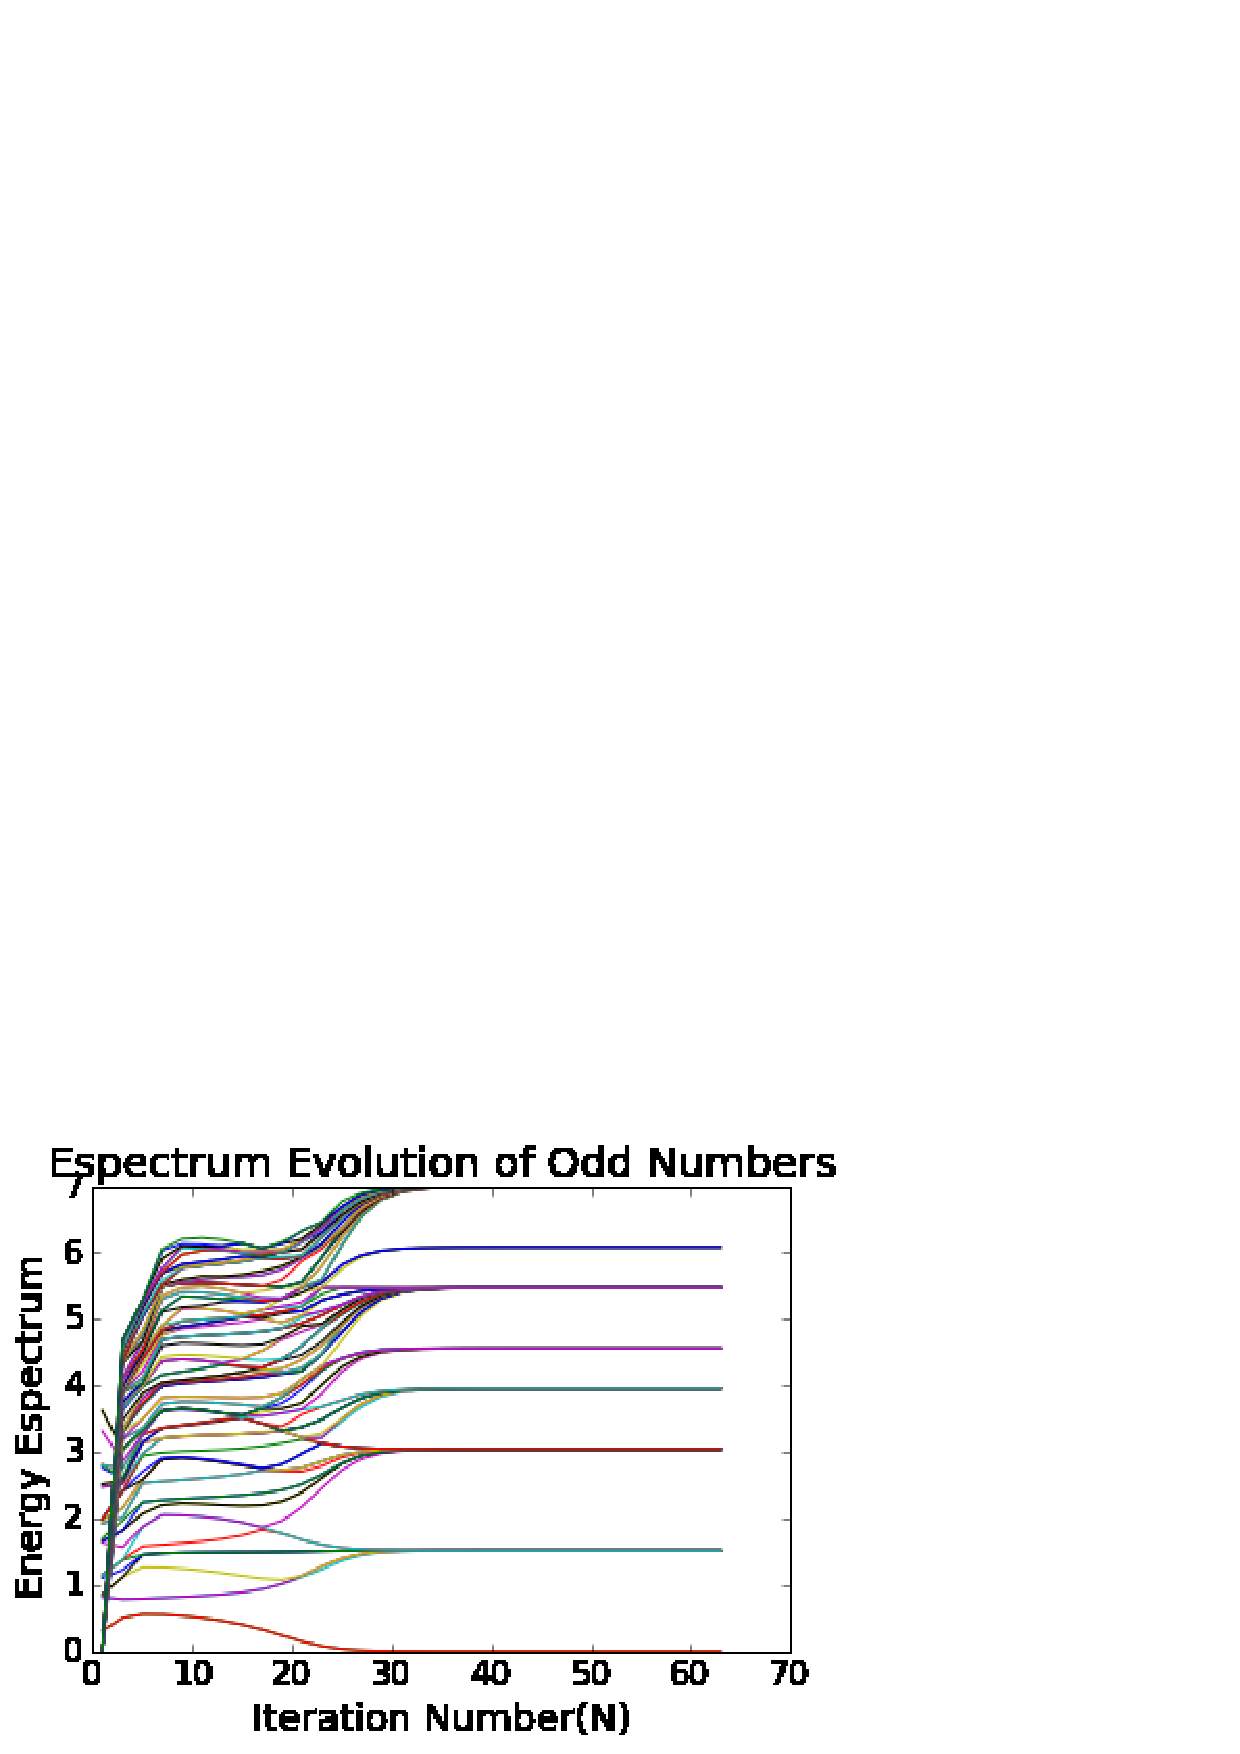
\includegraphics[scale=0.5]{IMAGES/odd.png}}\caption{\label{Fig-Dot-Spectrum} Evolution of the QD-spectrum vs number of
iterations of the code for $U=0.5,\ e_{d}=-0.25,\ \Gamma=2.82\times10^{-2}.$ }
\end{figure}

$H_{N=2,S=0}:$
\[
\begin{array}{c}
\vert\uparrow\!\downarrow\rangle\vert0\rangle\rightarrow\\
\vert\uparrow\rangle\vert\downarrow\rangle\rightarrow\\
\vert\downarrow\rangle\vert\uparrow\rangle\rightarrow\\
\vert0\rangle\vert\uparrow\!\downarrow\rangle\rightarrow
\end{array}\left[\begin{array}{cccc}
2\epsilon_{d}+\frac{3U}{2} & \Gamma & -\Gamma & 0\\
\Gamma & \epsilon_{d}+\frac{U}{2} & 0 & \Gamma\\
-\Gamma & 0 & \epsilon_{d}+\frac{U}{2} & -\Gamma\\
0 & \Gamma & -\Gamma & \frac{U}{2}
\end{array}\right]
\]


\begin{multicols}{2}

$H_{N=3,S=\frac{1}{2}}:$
\[
\begin{array}{c}
\vert\uparrow\!\downarrow\rangle\vert\uparrow\rangle\rightarrow\\
\vert\uparrow\rangle\vert\uparrow\!\downarrow\rangle\rightarrow
\end{array}\left[\begin{array}{cc}
\epsilon_{d}+\frac{U}{2} & -\Gamma'\\
-\Gamma' & \frac{U}{2}
\end{array}\right]
\]


$H_{N=3,S=\frac{-1}{2}}:$
\[
\begin{array}{c}
\vert\uparrow\!\downarrow\rangle\vert\downarrow\rangle\rightarrow\\
\vert\downarrow\rangle\vert\uparrow\!\downarrow\rangle\rightarrow
\end{array}\left[\begin{array}{cc}
\epsilon_{d}+\frac{U}{2} & -\Gamma'\\
-\Gamma' & \frac{U}{2}
\end{array}\right]
\]


\end{multicols}

Finally, we proceed to diagonalize $H_{0}$ by blocks $H_{N,S}$.
The resulting eigenvectors will be characterized by both quantum numbers
so that we can write them in the form $\vert N,S,i\rangle$ with $i$
takes as many values as the degeneracy of its block. For higher values of $N$,
the general formula for equation \prettyref{eq:H0fromH-1} looks as 
\begin{equation}
H_{N+1}=\Lambda^{\frac{1}{2}}\left[H_{N}+\frac{1}{2}\left(1+\Lambda^{-1}\right)\xi_{N}\left(f_{N\sigma}^{\dagger}f_{N+1,\sigma}+f_{N+1\sigma}^{\dagger}f_{N\sigma}\right)\right].\label{eq:NRG-Iteration Hamiltonians}
\end{equation}


We now proceed by induction supossing that for each $N$ the Hamiltonian $H_{N}$ is already diagonalized and the eigenvectors are organized in states with labels $\vert N,S,i\rangle.$ The next step will be to add the $4$-Hilbert space corresponding to $f_{N+1,\sigma}$ organized the eigenvectors according to the quantum numbers $\vert N',S',i\rangle$ and proceed to diagonalize by blocks the new Hamiltonian. Apart of it, the code must have a cutoff to the number of states. \\

This NRG code was previously implemented in C++ language by the advisor of this thesis. In \ref{Fig-Dot-Spectrum} we observe the evolution of the spectrum of the Hamiltonian according to the number of iterations of the code. As we can appreciate, this evolution converges for even and odd number around $N=30$.  \\



\subsection{Density Matrix Renormalization Group (DM-NRG)}
To compute  dynamical quantities \cite{costi_transport_1994} like the density of states  is the DMNRG \cite{hofstetter_generalized_2000}. 
\Jesus{Sill planning this section }

\subsection{NRG results in a Double Quantum Dot}
We ran the NRG code for the DQD with the following set of parameters:


$$  U_{1,2} = -2\ed{1,2} = 8.62\Gamma_1$$

\ref{fig:NRG-DQD} shows the NRG results for the density of states of QD1 in different states. The three plots show the external Coulomb peaks at $e_1 = \frac{U}{2} \sim 8.62\Gamma_1$, which represent the DOS of the energy levels. In addition  Figure \ref{fig:NRG-1D} shows a central peak at the fermi energy. \textbf{This is the Kondo Peak}. 

Figure \ref{fig:NRGDQD-G2} shows the DOS in the case where the two QDs are symmetrically attached.  At low energies, the inset shows the appearance of two satellite peaks representing the Ruderman-Kittel-Kasuya-Yosida (RKKY) interaction. This interaction is explained for this particular case in section \ref{sec:DoublePeak}.  

Again, the most interesting case is in Figure \ref{fig:NRGDQD-tdots}. The additional interference with the second dot completely destroys the Knondo effect. This effect is observed at energies closed to $t_{dots}=0.689\Gamma$ and  will take its relevance in the last chapter. 





%There is a problem with thes plots in xlabel.
\begin{figure}[t]
     \centering
    \subfloat[  \label{fig:NRG-1D}]{\includegraphics[scale=0.5]{IMAGES/DQD/NRG-QD.png}}
     \subfloat[$\Gamma_2 = \Gamma_1$ . Inset: Low energy DOS. \label{fig:NRGDQD-G2}]{\includegraphics[scale=0.42]{IMAGES/DQD/NRG-DQD.png}} 
    \subfloat[\label{fig:NRGDQD-tdots} $t_{dots}=0.689\Gamma$. Low energy DOS. ]{\includegraphics[scale=0.4]{IMAGES/DQD/NRG-IndirectDQD.png}}
    
     \caption{\label{fig:NRG-DQD} Density of states in QD1 predicted by NRG at each case. . The insets show the.  Note that figure a) is in a different scale due to a major central peak .. \protect\Source{ By the Author  }}
\end{figure}

% 
\chapter{Motivation}
\section{Majorana Fermions}

The  Majorana Fermions, so called in the name of the Italian physicist Ettore Majorana, where first defined in the attempt to find a real solution of the Dirac equation. The real field that solves this equation $\Psi_M$ , describes a fermion which is its own antiparticle. Hence it has no electric charge nor mass.  Till these days, no fundamental particle with these characteristics has been observed. However, in the last few years, there has been a huge speculation about the possibility of finding Majorana Fermions as a quasiparticle inside certain condensed matter systems. 

One of the most famous examples of these systems is the Kitaev chain which is the main objective of the this subsection. 


\section{The Kitaev Chain}
The Kitaev chain is a toy model in tight binding that represents a  finite $p$-wave superconducting wire. The main Hamiltonian is given by 
\begin{equation}
H = \sum_{i} \left[ -t(a_i^{\dagger} a_{i+1} + a_{i+1}^{\dagger}a_i) -\mu a_i^{\dagger} a_{i} +  \Delta a_{i}a_{i+1} + \Delta^* a_{i+1}^{\dagger}a_i^{\dagger} \right].  \label{eq:kitaevHam}
\end{equation}

Where $\mu$ is the chemical potential, so that $\mu a_i^{\dagger} a_{i}$ is the energy associated to each free state. $t(a_i^{\dagger} a_{i+1} + a_{i+1}^{\dagger}a_i)$ represents the interaction between neighbouring sites which is determined by the hopping term $t$. The remaining terms describe the superconducting properties of the system as is is established by the BCS theory of superconductivity. $\Delta$ is a complex superconducting parameter with the form  $\Delta = e^{i\theta} \super$. The associated terms represent the Cooper pairs which can be created or annihilated at neighbouring sites of the system.

The form of hamiltonian \prettyref{eq:kitaevHam} favors the possibility of introducing new operators $\gammaA{j}$ and $\gammaB{j}$ such that

\begin{equation}
\gammaA{j} = e^{i\theta /2}a_j+ e^{-i\theta/2 } \ann_j \ \ , \ \ \gammaB{j} = -i(e^{i\theta /2}a_j - e^{-i\theta/2} \ann_j).
\label{eq:majoranaTrans}
\end{equation}
It is simple check that these operators are self-adjoint $(\gammaA{j}^\dagger = \gammaA{j}, \gammaA{j}^\dagger = \gammaB{j})$. This is a required constraint for the Majorana particles. In addition they satisfy the fermionic anti-commutation relations
\begin{equation}
\begin{aligned}
\{\gammaA{i}, \gammaA{j}\} = \{ & \gammaB{i} , \gammaB{j}\} = 2\delta_{ij}  ,\\ 
  \{\gammaA{i}, \gammaB{j} & \} =0.
\end{aligned} 
\label{majoranaRel}
\end{equation} 
This allows us to understand the operators $\gammaA{i} , \gammaB{i}$ as majorana fermions. If we also take the inverse of \prettyref{eq:majoranaTrans} we obtain that each  (Dirac) fermion in Hamiltonian \eqref{eq:kitaevHam} is composed by two majorana fermions such that 
$$a_j = \frac{e^{-i\theta/2}}{2}(\gammaA{j}+ i\gammaB{j})$$
We could even adventure to say that these majorana operators are actually dividing the Dirac fermions into real($\gammaA{}$) and imaginary $(\gammaB{})$ part ,the same way as complex numbers are a composite of two real numbers. 

The new Kitaev Hamiltonian in the Majorana representation looks like 

\begin{equation}
H = \frac{i}{2} \sum_{j} \left[ -\mu \gammaA{j}\gammaB{j}  + (t- \super) \gammaB{j}\gammaA{j+1} + (t+ \super) \gammaA{j}\gammaB{j+1} \right]+Const,\label{eq:HamMajorana}
\end{equation}

Depending on the values of parameters $\mu, t$ and $\super$ we can identify two regimes represented by the following situations:


%\begin{figure}[t]
%$$\includegraphics[scale=0.5]{KitaevtopPhases.jpg}
%\centering
%\label{top.phases kitaev}
%\caption{{\small \textit{Taken from \cite{bernevig2015topological}. Ilustration of the Kitaev chain for open boundary conditions in the Majorana representation. a)Represents the trivial case where the hopping and the superconducting term approaches to $0$. b) The non-trivial topological phase. The coupling is produced between Majoranas in different Dirac fermions }}}
%\end{figure}


\begin{enumerate}
\item{If $\super = t = 0, \mu <0$} Hamiltonian \eqref{eq:HamMajorana} becomes $\frac{-i\mu}{2} \sum_{j} \gammaA{j}\gammaB{j}$ which represents the coupling of the Majoranas in the same Dirac fermion. (See figure \ref{top.phases kitaev} (a))

\item{If $\super = t > 0, \mu =0$} the situation is much more interesting. The Hamiltonian \eqref{HamMajorana} takes the form $H = 2ti\sum_{j} \gammaA{j}\gammaB{j+1}$. This implies that the coupling is performed between  Majoranas of different Dirac fermions leaving the edge Majorana operators ($\gammaA{1}$ and $\gammaA{2}$) uncoupled . This produces a new degeneracy in the ground state due to the emergence of a state produced by the uncoupled Majorana operators. The new state is localized at the edges of the chain.(See figure \ref{top.phases kitaev} (b)) 
\end{enumerate}

\chapter{Coupling the Majorana Zero Mode to a Double Quantum Dot \label{chap:Results} }
%--------------------------------------------------------------------------
\begin{figure}[hbt]
    \centering
    \includegraphics[scale=0.4]{IMAGES/GenModel.png}
    \caption{\label{fig:GenModel} Model for the DQD-Majorana system. Solid lines: Hopping interactions ($t_{dots}$: inter-dot coupling , $V_1,V_2$ couplings of QD1 and QD2 with the lead. ). Dashed lines: Majorana spin-$\dw$ effective couplings \eqref{eq:MajoranaCoupling} $t_1,t_2$. The atomic energy levels appear inside each QD $\ep_1, \ep_2$ are tuned by the gate voltages. The coulomb interaction is represented by $U_1,U_2$.  The red dashed horizontal lines represent the Fermi level. \protect \Source{ } } 
\end{figure}

\noindent The DQD-Majorana model is the most fundamental structure where Majorana manipulation is possible. Tunneling Majorana modes in this device have already inspired a few theoretical studies \cite{silva_andreev_2016,ivanov_coherent_2017} and experimental setups confirming the observations of Andreev molecules \cite{su_andreev_2017}. However, there is still no complete analysis of the transitions of the Majorana signatures between the QDs in this model, even though quantum tunneling of a MZM into a double dot offers several possibilities for MZM manipulation.  

 In this chapter, we will explore  different possibilities for Majorana manipulation in a device consisting of a DQD coupled to a MZM and a metallic lead (See \ \ref{fig:GenModel}). The simplicity of this model allows us to explore analytically different geometries of QD's from linear and symetric couplings to T-junctions (Fig.\ \ref{fig:MajoranaModels}). As in the previous models , we will consider both non-interacting and interacting regimes. 


% Tunneling of a MZM into a double dot shows several possibilities for manipulation of MZM,  there is still no complete analysis of the transitions of the Majorana signatures between the QDs in this model. 


% \noindent The idea of using Majorana islands formed by QDs coupled to topological superconducting wires has recently turned on new lights  into the fabrication of of quantum architectures \cite{barkeshli_physical_2015,karzig_scalable_2017}. The main insight  of this method is that today’s precise experimental control over the parameters of QDs -energy levels, tunneling couplings, etc.- offers the unique possibility of manipulating the Majorana modes inside multi-dot systems. The simplest case where Majorana manipulation is possible is in a double quantum dot. So far, no complete analysis of this basis case has been done. The purpose of this chapter is to fill this gap by realizing a full quantum transport study of the effects of coupling a Majorana mode with a double quantum dot. For this, we combine the ballistic transport and the NRG approach developed in \ref{chap: Methods}. 


% As previously stated in the , Majorana-QD  architectures turn on new lights to the area of topological quantum computing. 



% Using the ideas from the previous chapters we are going to test if it is possible to manipulate the Majorana zero mode in the double quantum dot.  

% In the previous chapter we observed the result of coupling a Majorana mode to a quantum dot. The Majorana signature characterized by a decay of the Fermi peak to the half of its original height is a



 The model in \ref{fig:GenModel} can be described from the combination of the Hamiltonians of a QD-Majorana system \eqref{eq:QD-Mham} and a DQD \eqref{eq:HDQD}. Integrating these models we obtain

\begin{equation}
H =\sum_{i=1}^2\sum_{k,\sigma}\left(\epsilon_{i}+\frac{U_i}{2}\right)d_{i\sigma}^{\dagger}d_{i\sigma}+ \frac{U_i}{2}(d_{i \sigma}^{\dagger}d_{i \sigma}-1)^{2} + t_i\gamma d_{i,\dw} + V_id^\dagger_{i\sigma}c_{k\sigma}+ t_{d o t s}d_{1 \sigma}^{\dagger} d_{2 \sigma} +\text{h.c}.
\label{eq:Generalmodel}
\end{equation}

Where $V_1,V_2$ is the coupling of dots $1,2$ to the lead. $t_1,t_2$ define the Majorana couplings with each dot. $t_{dots}$ is the inter-dot coupling. $\ep_1,\ep_2$ are the energy levels of the dot, which are tuned by the the gate voltage and $U_1,U_2$ are the coulomb repulsion parameters. 
% \Jesus{I neglected $\epsilon_M$ in this case. Depending on the future NRG results I will choose to add it or leave it that way. }



\section{Applying our methods to the DQD-Majorana system}


% In order to understand the physical properties of this model, we probed a set of thought processes. The main variable in this analysis is the density of states.  We  will observe its evolution on both QDs under the tuning of the model parameters such as the majorana couplings ($t_1 , t_2$)  ,  gate voltages ($\ed{1} , \ed{2} $) and the inter dot coupling ($t_{dots}$). With these processes intend to show whether it is possible to "manipulate" the majorana modes inside the dots by tuning the established parameters. The number of possible combinations of parameters is huge and not all of them lead to important results. So on, we used the ballistic transport to select which arrangements could bring novel results. The most interesting models were simulated with NRG in the interacting case \ref{fig:MajoranaModels}.  

\subsection{Non-interacting Green function:}

%  To solve the transport equations using the graph method from \ref{sec:GraphMethod} first not that 
This new model is a combination between the DQD  (\ref{fig:graphDQD}) and the Majorana-QD  \ref{fig:green-M-QD}(b). We can use the trick in \ref{sec:GreenMaj-DQD} to get rid of the Green function $\Green{f_\dw,d^\dagger_1}$ for the second Majorana operator. This allows us to obtain the following transport equations 
 
 
 
%  As we did previously in \ref{sec:GreenMaj-DQD} the transport equations for $f_\dw$ and $f^\dagger_\dw$ are 
% \begin{align}
%         \left(\omega-\epsilon_{M}\right)\Green{f_{\downarrow},d_{1\downarrow}^{\dagger}}&=\frac{t}{\sqrt{2}}\left(\Green{d_{1\downarrow},d_{1\downarrow}^{\dagger}}-\Green{d_{1\downarrow}^{\dagger},d_{1\downarrow}^{\dagger}}\right) \\
%     \left(\omega+\epsilon_{M}\right)\Green{f_{\downarrow}^{\dagger},d_{1\downarrow}^{\dagger}}&=\frac{t}{\sqrt{2}}\left(\Green{d_{1\downarrow},d_{1\downarrow}^{\dagger}}-\Green{d_{1\downarrow}^{\dagger},d_{1\downarrow}^{\dagger}}\right),
% \end{align}
% \noindent which allows us to take $\Green{f_{\downarrow}^{\dagger},d_{1\downarrow}^{\dagger}} = \frac{\omega + \epsilon}{\omega -\epsilon}\Green{f_{\downarrow}^{\dagger},d_{1\downarrow}^{\dagger}} $. Therefore, we can eliminate $\Green{f_{\downarrow}^{\dagger},d_{1\downarrow}^{\dagger}} $ from the equations even before we start Gauss-Jordan process.
 
 \begin{equation}
     \left[\begin{array}{ccccccc}
\omega-\epsilon_{1} & -V_{1}^{*} & -t_{dots} & -T_{1} & 0 & 0 & 0\\
-V_{1} & \omega-\epsilon_{k} & -V_{2} & 0 & 0 & 0 & 0\\
-t_{dots}^{*} & -V_{2}^{*} & \omega-\epsilon_{2} & -T_{2} & 0 & 0 & 0\\
-T_{1}^{*} & 0 & -T_{2}^{*} & \omega-\epsilon_{M} & T_{2}^{*} & 0 & -T_{1}\\
0 & 0 & 0 & T_{2} & \omega+\epsilon_{2} & V_{2}^{*} & t_{dots}^{*}\\
0 & 0 & 0 & 0 & V_{2} & \omega+\epsilon_{k} & V_{1}\\
0 & 0 & 0 & T_{1} & t_{dots} & V_{1}^{*} & \omega+\epsilon_{1}
\end{array}\right]\left[\begin{array}{c}
\Green{d_{\mathbf{1\downarrow}},d_{1\downarrow}^{\dagger}}\\
\Green{c_{k\downarrow},d_{1\downarrow}^{\dagger}}\\
\Green{d_{2\downarrow},d_{1\downarrow}^{\dagger}}\\
\Green{f_{\downarrow},d_{1\downarrow}^{\dagger}}\\
\Green{d_{2\downarrow}^{\dagger},d_{1\downarrow}^{\dagger}}\\
\Green{c_{k\downarrow}^{\dagger},d_{1\downarrow}^{\dagger}}\\
\Green{d_{1\downarrow}^{\dagger},d_{1\downarrow}^{\dagger}}
\end{array}\right]=\left[\begin{array}{c}
0\\
0\\
0\\
0\\
0\\
0\\
1
\end{array}\right],
 \end{equation}
 
 where $T_i = \frac{t_i}{\sqrt{\omega+\epsilon_M}}$. 
 
 
% ------------------------FIGURE GRAPH--------------------
     \begin{figure}[bt]
    \centering
    \includegraphics[scale=0.4]{IMAGES/Graphs/FinalGraph.png}
    \caption{\label{fig:Graph-MDQD} Graph method applied to a DQD coupled to a Majorana zero mode. a) Initial stage. b) Eliminated vertexes $c^\dagger_k$, $c_k$, $d_{2, \downarrow}$ , $d^\dagger_{2, \downarrow}$ in that order. c) Eliminated vertexes $d^\dagger_{1, \downarrow}$ and $f_\dw$, the final energy is $\omega-\Green{d_1,d_1^\dagger}$  . \protect\Source{   }} 
    \end{figure}

% ------------------------FIGURE GRAPH---------------------------
 The graph representing this equation is in  \ref{fig:Graph-MDQD}(a). Using the algorithm in \ref{sec:Algorithm} we start eliminating vertexes $c_k,c^\dagger_k, d_{2,\dw}$ and $ d^\dagger_{2,\dw}$ in that order. The self-energies associated to $d_{1,\dw}$ and $d^\dagger_{1,\dw}$ will be similar to the energy of the DQD \eqref{eq:EnDQD} giving 
\begin{equation}
    \epsilon_{DQD}^{\pm}=\pm\epsilon_{1}+\sum_{\mathbf{k}}\frac{V_{1}V_{1}^{*}}{\omega-\epsilon_{\mathbf{k}}}+\frac{\left\Vert \pm t_{dots}+\sum_{\mathbf{k}}\frac{V_{1}V_{2}^{*}}{\omega-\epsilon_{\mathbf{k}}}\right\Vert ^{2}}{\omega\mp\epsilon_{2}-\sum_{\mathbf{k}}\frac{V_{2}V_{2}^{*}}{\omega-\epsilon_{\mathbf{k}}}}. \label{eq:epDQD}
\end{equation}
\noindent There is also a correction in the couplings between the Majorana mode and $d_{1,\dw}$, $d^\dagger_{1,\dw}$ given by 

\begin{equation}
    T_{\pm}=\pm t_{1}\pm t_{2}\frac{\left(\pm t_{dots}+\sum_{\mathbf{k}}\frac{V_{1}V_{2}^{*}}{\omega-\epsilon_{\mathbf{k}}}\right)}{\omega\mp\epsilon_{2}-\sum_{\mathbf{k}}\frac{V_{2}V_{2}^{*}}{\omega-\epsilon_{\mathbf{k}}}}. \label{eq:T+-}
\end{equation}

\noindent In addition, since the Majorana is in contact with dot $2$, there is an extra-term appearing in the  Majorana self-energy given by 
\begin{equation}
    \epsilon_{M2}=\omega-\epsilon_{M}-\frac{\frac{\omega}{\omega+\epsilon_{M}}\left\Vert t_{2}\right\Vert ^{2} } {\omega-\epsilon_{2}-\sum_{\mathbf{k}}\frac{V_{2}V_{2}^{*}}{\omega-\epsilon_{\mathbf{k}}}}-\frac{\frac{\omega}{\omega+\epsilon_{M}}\left\Vert t_{2}\right\Vert ^{2}}{\omega+\epsilon_{2}-\sum_{\mathbf{k}}\frac{V_{2}V_{2}^{*}}{\omega+\epsilon_{\mathbf{k}}}}. \label{eq:M2}
\end{equation}
It only remains to eliminate out vertexes $d^\dagger_1$ and $f_\dw$  to obtain the green function 

\begin{equation}
    G_{{d_{1\downarrow},d_{1\downarrow}^{\dagger}}}\left(\omega\right)=\frac{1}{\omega-\epsilon_{DQD}^{+}-\frac{\left\Vert T_{+}\right\Vert ^{2}}{\omega-\epsilon_{M2}-\frac{\left\Vert T_{-}\right\Vert ^{2}}{\epsilon_{DQD}^{-}}}}.
    \label{eq:Green_NonInteracting}
\end{equation}

This simple formula summarizes the transport information through the first dot of the non-interacting Majorana-DQD system.  To compute the DOS we just need to replace  $\sum \frac{V_iV^*_i}{\omega -\epsilon_k}= -i\Gamma_i$ as performed in \ref{sec:GraphMethod}. By plotting the final DOS in Mathematica we were able to observe the transitions of the Majorana mode under manipulation of the model parameters.  


\subsection{NRG for the interacting system}

The Numerical Renormalization Group (NRG) technique described in \ref{sec:The-Numerical-Renormaliztion} is the most successful methods to study interacting quantum impurity models. In this model, the impurity is described by the DQD attached to the MZM. In our code, we set a Coulomb repulsion factor of $U =17.3\Gamma_1$ in both dots and a cut-off energy of $D=2U=34.6\Gamma_1$. The spacing with other energy levels is assumed to be higher than $D$, such that only the two coulomb states are relevant for the system dynamics.  When  $\epsilon_i = \frac{U}{2}$ in both dots, the system is in the Particle-Hole-Symmetric region. At this point, each dot has an odd number of electrons, hence, at sufficiently low temperature the system will exhibit characteristic Kondo peaks at the Fermi energy \cite{wilson_renormalization_1975}. The coexistence of Kondo and Majorana zero modes is still a point of contention in the area that has never been studied in DQDs and one of the objectives of this part of the project.


% Observing how the Kondo-effect interacts with the Majorana signature in the double quantum dot is also an insight of this project. 


To  improve the efficiency of the code we used the symmetries of the system to maintain a block structure during NRG's iterative diagonalization process. This model preserves the spin-$\up$ particle number $\hat{N}_\up$ and the spin-$\dw$ parity $\hat{P}_\dw = \pm $ ($+$ even, $-$ odd). The spin-$\dw$ particle number is not preserved due to superconducting-type Majorana coupling  \eqref{eq:MajoranaCoupling} . The initial Hamiltonian is organized in blocks according to these symmetries. This block structure is preserved during the entire iteration process \cite{bulla_numerical_2008}. To compute the spectral functions, we use the density matrix renormalization group (DM-NRG) described in \ref{subsec:DM-NRG} in combination with the Z-trick method \cite{oliveira_generalized_1994}, which improves spectral resolution at high energies.


To initialize the model in \ref{fig:Code} we set $H_{-1}$ equal to 
\begin{equation}
H_{-1} =\sum_{i=1}^2\sum_{k,\sigma}\left(\epsilon_{i}+\frac{U_i}{2}\right)d_{i\sigma}^{\dagger}d_{i\sigma}+ \frac{U_i}{2}(d_{i \sigma}^{\dagger}d_{i \sigma}-1)^{2} + t_i(\gamma d_{i,\dw}+d^\dagger_{i,\dw}\gamma)+t_{d o t s}\left(d_{1 \sigma}^{\dagger} d_{2 \sigma}+d_{2 \sigma}^{\dagger} d_{1 \sigma}\right),
\label{eq:imp_Ham}
\end{equation} 
\noindent and wrote the Hamiltonian in the symmetry-block diagonal representation (see \ref{sec:Double-Dot-Majorana-Hamiltonian.}). We also include manually the Hamiltonian $H_0$ into the code (See \ref{fig:Code}) to guarantee that both quantum dots are coupled to the first site of the chain. After this, the code follows the standard NRG algorithm and prints the density matrices to initialize DM-NRG. The final result is the spectral density which contains sufficient physical information to study the MZM-DQD model. In the following section, we show how the density of states can be used to simulate the Manipulation process of an MZM inside the DQD. 




\section{Manipulation of Majorana zero modes}


\begin{figure}[bt]
\centering
\includegraphics[scale=0.7]{IMAGES/DQD-M/3Model.png}
\caption{\label{fig:MajoranaModels}. \protect\Source{}} 
\end{figure}


The density of states provides significant information about the presence of a Majorana zero modes in the dot. We characterize the Majorana signature by a robust zero-mode with two possible heights:
 \begin{itemize}
         \item \textbf{Type I: }  The spin-$\dw$ DOS is the half of the spin-$\up$ DOS  at the Fermi energy $(\rho_\dw(0)=\rho_\up(0))$. 
         \item \textbf{Type II: } A spin-$\dw$ zero mode of height $ \rho_\dw(0) = \frac{0.5}{\pi  \Gamma_1}$. 
     \end{itemize}
In our results we observe several times these two types of signatures. Type I often appears when there is a zero-mode in the spin-$\up$ DOS, which is caused by the Kondo effect in the interacting case. Type II emerges in the remaining situations. 

We call MZM manipulation to the "movements" attributed to the Majorana signature under the tunning of the dot gate voltages $( \epsilon_1 , \epsilon_2 )$. This manipulation process is performed in three different set ups that are presented in \ref{fig:MajoranaModels} with definite values of $\Gamma_2$, $t_{dots}$, $t_1$ and $t_2$. In configuration (a), we coupled the QD symmetrically to the lead and the Majorana mode. With this setup we expect to break the localization of the MZM which should split and tunnel into both dots. In setups (b) and (c) we coupled the second dot indirectly through the first dot. Hence, quantum  interference should split the zero mode in two states. Our objective is to observe what occurs with the Majorana signature in this situation. There are two options to connect the MZM in this situation. Attached it directly through the first dot (b) or indirectly through the second dot (c). Both alternatives are geometrically distinct since (b) suggests a T-junction coupling while (c) reflects a connection  in series of both QD's between the lead and the MZM. 


 %-----------F I G U R E  t1 = t2 ------
\begin{figure}[H]
    \begin{center}
    \includegraphics[scale=0.36]{IMAGES/GreenResults/t1=t2.png}
    \caption{ \label{fig:t1=t2}  Non-interacting DOS in the symmetric coupling(\ref{fig:MajoranaModels}(a)) at each QD. First column: Dot 1. Second column: Dot 2. The gate voltages vary at each row.  First row: Zero-bias in both dots $\ep_1=\ep_2=0$. Second row: $\ep_1=5\Gamma_1, \ \ep_2 =0$.  Third row: $\ep_1=0, \ \ep_2 =-5\Gamma_1$.  Bold blue lines: Spin-$\up$ DOS. Thin red lines: Spin-$\dw$ DOS. The insets at the right show which dot carries a Majorana signature, represented by a red dashed circle. Upper: First dot. Lower: Second dot. \protect\Source{}
    }
    %
    \end{center}
\end{figure}
%-----------F I G U R E  t1 = t2 ------

\subsection{Non-interacting manipulation}

 The non-interacting results for setups (a),(b) and (c) of \ref{fig:MajoranaModels} are shown at figures \ref{fig:t1=t2}, \ref{fig:t1>0} and \ref{fig:t2>0} respectively. Each figure depicts the DOS of dot $1$(left) and dot $2$(right). The gate voltage is initially $0$ in both dots at the first row. In the second row, the gate voltage is turned on to  $\epsilon_1 = 5\Gamma_1$ , while the second dot remains at $\epsilon_2 = 0$ . In the third row the first dot's voltage is off $\epsilon_1=0$ and we switch on the second dot with a negative voltage of $\epsilon_2 = -5\Gamma_1$. The inset figures at the right side of each row show which dots exhibit Majorana signatures, depicted by a red dashed circle inside the dot. These images will continuously change under the tuning of gate voltages which represents the manipulation of the Majorana signature.



In \ref{fig:t1=t2} we observe the results for the symmetric coupling setup \ref{fig:MajoranaModels}(a). In the particle hole symmetric case (first row) the DOS is equal in both dots. Note that the spin-$\dw$ (Thin red line) DOS is the half of the spin-$\up$ (Bold blue line) DOS at the Fermi energy $(\rho_\dw(0) = \frac{1}{2}\rho_\up(0))$. This type II Majorana signature is similar to the one observed when a single dot is coupled to a Majorana mode. \cite{liu_detecting_2011} We may conclude that the Majorana in tunneling inside both dots breaking the localization of the MZM. If a positive or negative gate voltage is induced in one of the dots, as shown in the second and third row of \ref{fig:t1=t2}(c)-(f),  the Majorana zero mode vanishes from that dot. Meanwhile the density of states in the other dot increases while preserving the Majorana signature. This means that the MZM is actually being induced to "leave" this dot and leak into the other by the biased voltage. This is the  first example of MZM manipulation. 


 %-----------F I G U R E  t1 >0 ------
\begin{figure}[bt]
    \begin{center}
    \includegraphics[scale=0.36]{IMAGES/GreenResults/t1>0.png}
    \caption{  \label{fig:t1>0} Non-interacting DOS of the T-dot coupling \ref{fig:MajoranaModels}(b). (b). First line (a),(b): $\ep_1=\ep_2=0$. Second line (c),(d): $\ep_1=5\Gamma_1$ , $\ep_2=0$. Third line (e),(f): $\ep_2=-5\Gamma_1$ , $\ep_1=0$.   Blue bold lines: Spin-$\up$ DOS. Red thin lines: Spin-$\dw$ DOS. The inset at the upper-right corner of each line indicates which dots  exhibit  Majorana signature, which is represented by a red dashed circle inside the dot. \protect\Source{}
    }
    %
    \end{center}
\end{figure}
%-----------F I G U R E  t1 >0 ------

Another example can  occur when the second dot is not directly connected to the lead. In this case, the inter-dot tunneling generates quantum interference which finally destroys the central peak as observed in \ref{fig:t1>0}(a) at the spin-$\up$ DOS . The spin-$\dw$ channel at \ref{fig:t1>0}(a), which is coupled to the MZM, does not exhibit the characteristic Fermi peak either. Instead, the one half Majorana signature at the Fermi energy $(\rho_\dw(0) = \frac{1}{2}\rho_\up(0))$ appears clearly inside the second dot \ref{fig:t1>0}(b). This situation prevails when the first dot's gate voltage is turned on \ref{fig:t1>0}(c)\&(d). While the first dot does not seem to exhibit any type of Majorana signature, the second dot's spin-$\dw$ DOS exhibits a robust zero-mode of height $\frac{0.5}{\pi \Gamma}$. The results are more exciting when the second dot's gate voltage is turned on in \ref{fig:t1>0}(e)\&(f). These figures clearly show how the MZM, previously localized at the second dot, is induced to leave this dot and to return into the first dot. Moreover, the DOS of spin-$\up$ and spin-$\dw$ channels are very similar to the spectral densities observed at \ref{fig:t1=t2}(d)(e), which means that the previous interference pattern has disappeared due to this gate voltage. 

 %-----------F I G U R E  t2 >0 ------
\begin{figure}[bt]
    \begin{center}
    \includegraphics[scale=0.45]{IMAGES/GreenResults/t2>0.png}
    \caption{  \label{fig:t2>0}  Non-interacting DOS of the set up in \ref{fig:MajoranaModels}(c).  First line (a),(b): $\ep_1=\ep_2=0$. Second line (c),(d): $\ep_1=5\Gamma_1$ , $\ep_2=0$. Third line (e),(f): $\ep_2=-5\Gamma_1$ , $\ep_1=0$.   Blue bold lines: Spin-$\up$ DOS. Red thin lines: Spin-$\dw$ DOS. The inset at the upper-right corner of each line indicates which dots  exhibit  Majorana signature, which is represented by a red dashed circle inside the dot. \protect\Source{}
    }
    %
    
    \end{center}
\end{figure}
%-----------F I G U R E  t2 >0 ------


The results of the third configuration \ref{fig:MajoranaModels}(c) appear in \ref{fig:t2>0}. Contrary to what was observed in the previous case, this time the Majorana signature is not destroyed by the interference but instead, the  $\frac{0.5}{\pi \Gamma}$-height MZM emerges indirectly in the first dot. This is a perfect way to separate the Majorana's spin-$\dw$ DOS from the central spin-$\up$ zero-mode which is still destroyed by the interference. In addition, the second dot still exhibits a type I Majorana signature as observed in \ref{fig:t2>0}(b). In the second row we observe that turning on the gate voltage in dot $1$  destroys the Majorana signature in both dots \ref{fig:t2>0}(c)(d). On the other hand, if the second dot's voltage is switched both dots will preserve their Majorana signature (QD1:type I, QD2: type II), while the spin-$\up$ quantum interference vanishes in the first dot.






% In this part we will discuss the three models in figure \ref{fig:Models} which are particularly interesting for the exotic behavior of their Majorana signature. The parameters $(t_1,t_2, t_dots)$ are fixed in these three models and we will take $\ep_1$ and $\ep_2$ as variables. The first model(a), represents a symmetric coupling of the DQD with the lead and the Majorana mode. In models (b) and (c) the second dot is indirectly coupled to the system through the first dot. As already analyzed in \ref{sec:GreedDQD}, the quantum interference generated by this coupling will destroy the central peak. The Majorana fermion can be either connected to the first dot (b) or to the second dot (c). The system will exhibit different Majorana signatures depending on which dot is connected to the Majorana zero mode.   



% On each case we observe three different situations. 
% \begin{itemize}
%     \item First Row: Zero bias. No gate $\ep_1 =\ep_2 = 0$.
%     \item Second Row: We turn on the first dot's gate voltage $\ep_1 = 5\Gamma_1, \ep_2 = 0$.
%     \item Third Row: We turn on the second dot's gate voltage $\ep_2 = -5\Gamma_1, \ep_1 = 0$.
% \end{itemize}

    

%     The density of states for the setup in \ref{fig:Models}.(a) is shown in Figure \ref{fig:SymCoupling}. Since the model is non-interacting, spin-$\up$ and spin-$\dw$ models are independent. The spin-$\dw$ DOS (dashed line) shows the effects caused by the Majorana zero-mode in comparison with the spin-$\up$  results (solid line). In the particle hole symmetric (first line) the DOS is equal in both dots. Note that that the spin-$\dw$ DOS is the half of the spin-$DOS$ at the fermi energy $\rho_\dw(0) = \rho_\up(0)$. This Majorana signature is similar to the one observed in the single dot case \cite{liu_detecting_2011}. We may conclude that the Majorana tunnels inside both dots. If a positive or negative gate voltage is induced in one of the dots, as shown in the second and third row of Figure \ref{fig:SymCoupling},  the Majorana zero mode vanishes. Looking to the other dot we can also observe that the Majorana signature in the other dot recovers the form observed in the single dot-Majorana model. Thus, by activating the gate voltage in one of the dots it is possible to induce the majorana mode to leave to the other dot.  

    
     
%     If the second dot is not directly connected to the lead the induced tunneling between both dots generates a path difference that destroys the central peak (See FIG\ref{fig:Interference} spin-$\up$ line). We can then proceed to connect the Majorana to each one of these dots. \ref{fig:Interference} shows the results of connecting the MZM to the first dot. Note that at zero-bias, quantum interference  destroys the Majorana mode in the first dot. However, in the second dot the spin-$\dw$ DOS is the half of the spin-$\up$ DOS at the Fermi energy, which is a clear Majorana signature. Hence, in this kind of arrangement the Majorana mode is allocated in the second dot.  \ref{fig:Interference}(e),(f) show that it is possible to reestablish the initial Majorana signature in the first dot by applying a gate voltage to the second dot. On the other hand, turning on the first dot's gate voltage does not lead to a meaningful change in the Majorana signature \ref{fig:Interference}(c),(d). While the spin-$\dw$ DOS in the first dot is still $0$ at the Fermi energy, the second dot shows a $0.5$-height zero mode. Although the spin-$\up$ DOS does not double the density of states any more, this signal is robust and equal in height to a Majorana signature which supports our claim that it is indeed a Majorana mode. 
%     If the Majorana mode is connected to the first dot, this interference will destroy the Majorana signature in the first dot. Interestingly, it is possible to observe a clear Majorana signature in the second dot characterized by a half central peak in the spin-$dw$ DOS. While turning on the first dot gate voltage seems to destroy this Majorana signature, tuning the second dots gate voltage returns the Majorana signature to the first dot. 


%     We now get into the final case that is when the Majorana mode is coupled to the second dot which is indirectly attached to the lead through the first dot. In this case \ref{fig:IndirectCoupling}(a)(b) shows that the Majorana signature is present in both dots, despite the Majorana is not directly coupled to the first dot. Moreover, we can observe that the spin-$\dw$ DOS is equal to $0.5$ at the Fermi energy while the spin-$\up$ peak has been destroyed by the interference. After turning on the first gate voltage we observe that the Majorana signature is destroyed in both dots \ref{fig:IndirectCoupling}(c)(d). This is totally opposite the results of increasing the second dot voltage which creates an stable $0.5$ Majorana signature at the Fermi energy of both dots \ref{fig:IndirectCoupling}(e)(f). 






\subsection{Interacting manipulation \label{sec:DQD-M-Interacting}}

 %-----------F I G U R E  t1=t2 ------
\begin{figure}[bt]
    \begin{center}
    \includegraphics[scale=0.52]{IMAGES/NRG/NRG-t1=t2.png}
    \caption{  \label{fig:NRG_Majorana}    Density of states of both dots in the symmetric coupling without gate voltages between the Majorana and the interacting DQD. Bold blue lines: Spin-$\up$ DOS. Thin red lines: Spin-$\dw$ DOS. Inset: Low-energy DOS.\protect\Source{}
    }
    %
    \end{center}
\end{figure}
%-----------F I G U R E  t1 =t2 ------

Now we consider a Coulomb repulsion energy of $U = 17\Gamma_1$ in both dots. The factor $ \frac{U_i}{2}(\sum_{\sigma} \hat{n}_{i\sigma}-1)^{2}$ in \eqref{eq:Generalmodel} favors states with an odd number of electrons (and holes). In addition, particle-hole equilibrium is now achieved when $\Delta \epsilon_{i} := \left(\epsilon_{i}+\frac{U_i}{2}\right)$.  Any induced gate voltage must be considered as a shifting $\Delta \epsilon_{i}$ from this equilibrium point. \ref{fig:NRG_Majorana} shows the DOS of both QDs for the symmetric coupling configuration \ref{fig:MajoranaModels}. The two peaks appearing at around $8.6\Gamma_1 = \frac{U_i}{2}$ represent the two energy levels spaced by the Coulomb repulsion factor $U$. The central spin-$\up$ peak is a consequence of the Kondo effect, \cite{hewson_kondo_1997,wilson_renormalization_1975}  while the two satellite peaks observed in the inset  are the result of the  RKKY indirect interaction between both dots.  \cite{ruderman_indirect_1954,kasuya_theory_1956,yosida_magnetic_1957} Moreover, the system presents a Majorana signature characterized by half spin-$\dw$ DOS at the Fermi energy $(\rho_\dw(0) = \frac{1}{2}\rho_\up(0))$  . Note, that in this case the Majorana signature coexists with the Kondo effect in the DQD as already predicted by Ruiz-Tijerina \textit{et al.} for a single dot. \cite{ruiz-tijerina_interaction_2015}


% If the two dots are interacting, with $U = 17.6\Gamma_1$, the spin-$\up$ density of states for the symmetric configuration (\ref{fig:Models}.(a)) is pretty similar to the DQD-symmetric model. The height of the central peak decays to $0.25$ and two new peaks appear corresponding to the dots anti-ferromagnetic interaction. In the spin-$\dw$ channel we can observe a zero mode with height equal to the half of the spin-$\up$ DOS. The effect of the Majorana coupling can be observed better on \ref{fig:2D/Shift_t1=t2}. 

\begin{figure}[H]
    \centering
    \includegraphics[scale=0.5]{IMAGES/NRG/FullEd2.png}
    \caption{\label{fig:ed2/Fermi} (a)-(d) Dependence of the density of states of setup in \ref{fig:MajoranaModels}(a) over $\omega$ and the gate voltage $\Delta \epsilon_2$ . $\Delta \epsilon_1=0$  Up: Dot 1. Down: Dot 2. Left: Spin-$\up$. Right: Spin-$\dw$.  (e) Evolution of the relation $\frac{\rho_\up(0)}{\rho_\up(0)}$ for both QDs. While QD2 losses rapidly the Majorana signature, QD1 maintains it till $\Delta \ed{2}\sim 5$. \protect\Source{}}
\end{figure}



    In this part of the project we are interested in the physics at low energy scales $\omega \sim \Gamma_1 $ close to the Kondo and MZM temperature \footnote{The MZM temperature $T_M$ can be defined by the energy scale $k_BT_M$ where the Majorana signature is visible. This effect has been plentifully discussed in a previous paper , together with its relationship with the Kondo temperature \cite{ruiz-tijerina_interaction_2015}. In the regime we are presenting in this thesis, the Majorana and Kondo temperature are similar, hence we are at an energy range where we can observe both effects co-existing. We will present further discussion about this idea in our DQD-Majorana model in a future paper.}. At this scale we can observe similar Majorana signatures compared with the non-interacting case. For instance, the inset \ref{fig:NRG_Majorana} shows the NRG results for the symmetric setup in \ref{fig:MajoranaModels}(a). In agreement with the non-interacting results, both dots have type I Majorana signatures. 

    When the gate voltage is turned on, we observe the number of holes $(\omega>0)$ increasing in the spin-$\up$, while the particles $(\omega<0)$ increase in the spin-$\dw$ (See \ref{fig:ed2/Fermi}(a)-(d) ). At $\Delta\epsilon_2 \approx 6\Gamma_1$, the Coulomb peak overlaps with the Fermi energy in the spin-$\downarrow$ channel, destroying the Majorana zero mode. This event is visible in \ref{fig:ed2/Fermi}(e), where the type one Majorana signature is clearly destroyed in Dot $1$ after $\Delta\epsilon_2 > 6\Gamma_1$. For $\Delta\epsilon_2 < 6\Gamma_1$ we observe an stable Majorana signature in dot $1$ with $\rho_\dw(0) \approx \frac{1}{2}\rho_\up(0))$. In the second dot the zero modes are absorbed by the dot, which slowly destroys the Majorana signature. 

     %-----------F I G U R E  7 ------
\begin{figure}[bt]
\begin{center}
\includegraphics[scale=0.5]{IMAGES/NRG/t1=t2.png}
\caption{ \label{fig:Nt1=t2} The same as in \ref{fig:t1=t2} for the  interacting DOS in the symmetric coupling  (\ref{fig:MajoranaModels}.\protect\Source{}
}
%
\end{center}
\end{figure}
%-----------E N D  F I G U R E  7 ------

    The red cuts in \ref{fig:ed2/Fermi} are plotted in \ref{fig:Nt1=t2} where we depict the results of Majorana manipulation. In agreement with the non-interacting case, the particle hole symmetric model receives both Majorana modes. Whenever a gate voltage is switched on, the Majorana is forced to tunnel into the other dot. We observe similar results for positive and negative gate voltages. 

 
 In the T-dot coupling \ref{fig:MajoranaModels}(b), the spin-$\up$ Kondo peak in  \ref{fig:Nt1>0} is destroyed by interference just as in the non-interacting case. This phenomenon had already been predicted for a T-junction of a double quantum dot attached to metallic leads \cite{dias_da_silva_transmission_2008}. The insight of our model is that an attached MZM should also disappear due to the same interference. Furthermore, a type I Majorana signature can be observed at very low energies in the inset of \ref{fig:Nt1>0}(b). However we have to recognize that both zero-modes decay significantly in the second dot. When the first voltage is turned on, the Majorana mode jumps onto the first dot which presents a type I Majorana signature. This is a clear difference with the non-interacting results where the Majorana signature stayed in the second dot.  If the second dot is switched on , a type II Majorana signature appears at very low energies in dot 1, which is coherent with the idea that the Majorana interference should disappear in this case. In \ref{fig:Nt1>0}(e) we identify emergence of a Fano resonance at the Fermi energy causing the sharp-asymmetric peak at $\omega = 0$. Fano resonances have already been documented in similar models in \cite{schuray_fano_2017}. We are going to talk more about this resonance in following section. 



 %-----------F I G U R E  4 ------
\begin{figure}[bt]
\begin{center}
\includegraphics[scale=0.4]{IMAGES/NRG/t1>0.png}
\caption{  \label{fig:Nt1>0} The same as in \ref{fig:t1=t2} for the  interacting DOS of the T-dot junction \ref{fig:MajoranaModels}(b). Inset in b): Zoom to low-energy DOS. \protect\Source{}
}
%
\end{center}
\end{figure}

\begin{figure}[H]
    \centering
    \includegraphics[scale=0.4]{IMAGES/NRG/c)LogEv-ed1.png}
    \caption{\label{fig:logc}  Logarithmic dependence of the density of states for interacting dots coupled in series  \ref{fig:MajoranaModels}(c) over $\omega$ and the gate voltage $\Delta \epsilon_1$. $\Delta \epsilon_2=0$. The dependence over $\Delta \epsilon_2$ produces similar results. \protect\Source{}}
\end{figure}



% -------------------FIGURES EVOLUTION ED--------------------
% \begin{figure}[h]
% \centering
% 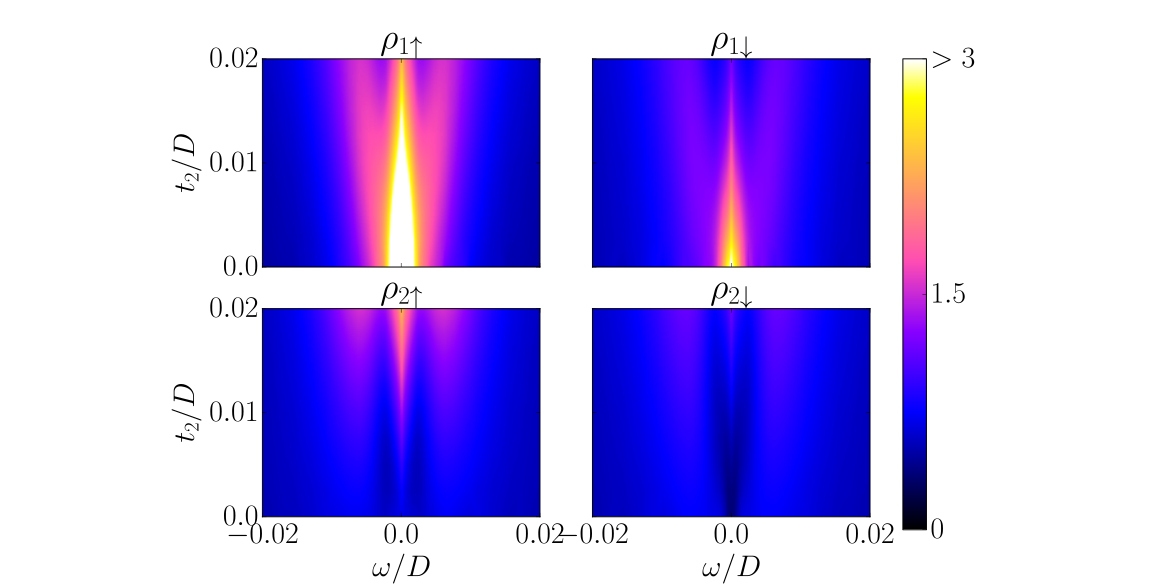
\includegraphics[scale=0.35]{IMAGES/ed2/2D.png}
% \caption{\label{fig:2D/Shift_ed2} Evolution of the DOS of both QDs through the $\ed{2}$ tuning. UP: QD1. DOWN: QD2. LEFT: Spin $\up$. RIGHT: Spin $\dw$.}
% \end{figure}



% -------------------FIGURES EVOLUTION ED--------------------


%-----------E N D  F I G U R E  4 ------
\begin{figure}[bt]
    \begin{center}
    \includegraphics[scale=0.41]{IMAGES/NRG/t2>0.png}
    \caption{  \label{fig:Nt2>0} The same as in \ref{fig:t1=t2} for the  interacting DOS for interacting dots coupled in series (\ref{fig:MajoranaModels}(c)). Inset in b): Zoom to low-energy DOS. \protect\Source{}
    }
    %
    \end{center}
    \end{figure}



    Finally, \ref{fig:Nt2>0} shows the NRG results for the last configuration, where the dots are coupled in series \ref{fig:MajoranaModels}(c). Notably, the indirectly-attached MZM exhibits a robust type II Majorana signature in the first dot over a destroyed Kondo peak. This is observed clearly in  \ref{fig:logc} where $\rho_{1\dw}$ exhibits a constant $\frac{0.5}{\pi \Gamma_1}$-height Majorana peak  . This signature is stable under the gate voltage tuning in dot $1$ and similar results are obtained in dot $2$ . In addition, only  in the particle hole symmetric case the second dot presents a type II Majorana signature (Inset \ref{fig:Nt2>0}(b)). 

    We could understand this effect by thinking that the dots in model (c) are attached in series. Therefore both QDs can be thought as extensions of the Kitaev chain, were the first dot is the last place in the wire. Hence the Majorana should be localized at this dot despite the application of gate voltages. This situation is similar to the case of a single dot attached to a Majorana chain, where it is known that the MZM appears in the dot even when this is supposed to be empty \cite{vernek_subtle_2014}. It still remains the doubt about why this effect is not observed in the non-interacting case . On the other hand, there is a Fano resonance at the Fermi energy in the spin-$\dw$ DOS  \ref{fig:Nt2>0}(d)(e) . This zero mode was not identified as a potential Majorana signature since it varies with the values of $\Delta \ep_1$ (\ref{fig:logc}) and $\Delta \ep_2$.
    

We are now writing a paper summarizing these results. As we observed, we were able to characterize the transitions of the Majorana signature in different geometric arrangements of the dots. In the following section we will present some ideas that are still in development. We hope they could lead us to future publications

\section{Additional  results}

\begin{figure}[t]
\centering
\includegraphics[scale=0.45]{IMAGES/NRG/Indirect.png}
\caption{\label{fig:indirect} Dependence of the DOS in the symmetric model \ref{fig:MajoranaModels}(a) over $t_1=t_2$ and $\omega$. Up: High energy . Down: Zoom to low energy states.  \protect\Source{}}
\end{figure}

This section contains additional results which we are considering to study in  future publications. 

\subsection{Indirect exchange through the Majorana mode}

In \ref{fig:NRG_Majorana} we observed the emergence of satellite peaks at low energies product of anti-ferromagnetic exchange interactions. This exchange interaction can occur through the lead and through the Majorana mode. The reason why we are observing just two satellites is because the Majorana  couplings $(t_1=t_2)$ and the broadening parameters $(\Gamma_1 = \Gamma_2)$ are about the same order. Hence the peaks are a superposition of both exchange interactions. 

We can separate both exchange interactions by observing the dependence of the DOS at different orders of $t_1=t_2$ in \ref{fig:indirect}. We can distinguish two regimes:

\begin{figure}[t]
\centering
\includegraphics[scale=0.5]{IMAGES/NRG/Lowt1=t2.png}
\caption{ \label{fig:indirectLow} Dependence of the DOS in the symmetric model \ref{fig:MajoranaModels}(a) over $t_1=t_2$ and $\omega$. Up: High energy . Down: Zoom to low energy states.  \protect\Source{}}
\end{figure}

\begin{enumerate}
 \item Low Majorana coupling $t_1=t_2 < 0.5$: Two additional satellite peaks appear in the spin-$\dw$ DOS (See inset in \ref{fig:indirectLow} for better appreciation). These peaks are similar to the  Kondo satellites that appear at high energies. However, since they appear only at low-energies, it is clear that they are produced by the MZM. We conclude that these two satellites are produced by the indirect exchange through the attached  Majorana quasi-particle. 
 \item High Majorana coupling $t_1=t_2 > 0.5$: When the Majorana coupling is high enough, the indirect exchange through the MZM occurs in the same energy scale as the Kondo satellites. Notably, the spin-$\dw$ satellite peaks in the high energy regime are not affected by this effect. Instead, a visible inflation of the satellites in the spin-$\up$ DOS is observed. Therefore the MZM is actually correlated with the spin-$\up$ DOS through the satellite peaks. This is unexpected since the Majorana is only coupled to the spin-$\dw$ channel.  The only explanation for this is that these satellites are formed by a strongly correlated state between the MZM, the dot states and the lead. 
\end{enumerate}
\begin{figure}[h]
\centering
\includegraphics[scale=0.64]{IMAGES/NRG/IND.png}
\caption{\label{fig:IND} DOS at both dots for the model in the left inset. The right inset zooms the low-energy DOS in the second dot.\protect\Source{} }
\end{figure} 

% \begin{figure}[t]
% \centering
% \includegraphics[scale=0.6]{IMAGES/NRG/Indirect.png}
% \caption{\label{fig:indirectLow} Dependence of the DOS in the symmetric model \ref{fig:MajoranaModels}(a) over $\omega$ for $t_1=t_2 = 0.1\Gamma_1$ (Low energy regime). Left inset: Majorana model. Right inset:Low energy regime. Majorana exchange peaks can be observed.  \protect\Source{}}
% \end{figure}



\subsection{Indirect Majorana coupling through the lead}

Imagine a model were we connect both dots symmetrically to the leads but we only connect the MZM to the first dot. In addition, we do not allow inter-dot tunneling. Then the only connection between the MZM and the second dot would be passing through the first dot and  the lead. We didn't expect to see any Majorana signature in the second dot in these conditions. However, \ref{fig:IND} shows a clear type I Majorana signature in the second dot.




 Note also that the density of states in the second dot is very small in comparison with the first dot. This is intriguing since this dot is directly connected with the lead and it is still at the Kondo regime. This ambiguity means that the zero-bias DOS is favored by a direct coupling to an MZM.  

\subsection{Critical behavior in  zero-bias DOS }

In \ref{fig:Nt1>0}(f) we observe a sharp peak at DOS. This peak is actually a big problem for our results since they are  supported on the spectral densities at the Fermi energy. In \ref{fig:Critical} we observe a critical behavior in the zero-bias DOS close to $\Delta\epsilon_2 =0$. This is quite intriguing . 


\begin{figure}[t]
\centering
\includegraphics[scale=0.5]{IMAGES/NRG/Critical.png}
\caption{\label{fig:Critical} Logarithmic dependence of the DOS in the second dot for setup in \ref{fig:MajoranaModels}(b) over the second gate voltage. Cut at $5\Gamma_1$ corresponds to \ref{fig:Nt1>0}(f). \protect\Source{} }
\end{figure} 



\chapter{Conclusions}


In this work, we developed two methods to study the system of a  double quantum dot attached to a Majorana chain. We probed successfully these methods in simpler cases such as the double quantum dot (\ref{sec:GreedDQD} , \ref{sec: NRG-DQD}) and the QD-Majorana system (\ref{sec:QD-Majorana}). The results obtained in these sections are in agreement with previous papers  regarding the Kondo interference in double quantum dots \cite{dias_da_silva_transmission_2008}, MZM leaking  into quantum dots \cite{,liu_detecting_2011} and the co-existence of Kondo-Majorana physics \cite{ruiz-tijerina_interaction_2015}. 

Moreover,  we introduced the Graph-Gauss-Jordan algorithm (\ref{sec:GraphMethod}) as a simple, didactic, analytical and graphical method to solve the equations of motion. This method allowed us to obtain exact expressions for the non-interacting Green functions at several stages of the project. In particular, in the double quantum dot - Majorana model it proved to be extremely useful to simplify the complexity of the solution given by a fractional polynomial of $9^\text{th}$-degree in up to 7 variables. Furthermore, with this expression we were able to predict interesting parameters for simulation in the interacting regime. We hope for its extended use in condensed matter physics.


In \ref{chap:Results} we used the methods from chapter \ref{chap: Methods} to study the transitions of the Majorana zero modes  inside a double quantum dot. Comparing the exact analytical solution in the non-interacting system and the NRG results for interacting quantum dots, we were able to characterized the displacements of the MZM inside the double quantum dot for the three setups in \ref{fig:MajoranaModels}, representing a symmetric coupling, a T-dot junction and a linear coupling of the dots. All of these manipulations are summarized in \ref{fig:ResultModels} . We observe a considerable agreement regarding the location of the Majorana signature between the interacting and non-interacting results with minor differences: 

\begin{itemize}
    \item Symmetric coupling \ref{fig:ResultModels} C.I : The MZM leaks inside both dots. For interacting dots, the Majorana signature will emerge near the Kondo temperature.   At this regime the system presents combined Kondo-Majorana physics . Additional satellite peaks produced by the indirect exchange through the lead and the MZM appear at low energies. If the gate voltage of one dot is turned on the MZM is induced to tunnel only into the other dot, which is the key to MZM manipulation. 
    \item T-dot coupling \ref{fig:ResultModels} C.II: The the spin-$\up$ zero mode at QD1 (The Kondo peak if the system is interacting) is destroyed by quantum interference with the second dot. This interference will also destroy the MZM in the first dot but a type I Majorana signature will still appear in the second dot. The Majorana mode can be induced to tunnel back into the first dot if a gate voltage is applied on the second dot. This signature is visible at very low energies (bellow $0.1\Gamma_1$) in the interacting case. 
    \item Dots coupled in series \ref{fig:ResultModels} C.III : An indirect type II Majorana signature is observed in the first dot. This signature is robust, specially in the interacting case, where it is present in all configurations, despite gate voltage tunning. Fano resonances emerge in the second dot. One of them seems to have critical behavior. 

\end{itemize}

    
    \begin{figure}
        \begin{center}
        \includegraphics[scale=0.4]{IMAGES/Graphs/Majorana_Old_Models.png}
        \caption{  \label{fig:ResultModels} Table of Majorana signatures in the studied cases in interacting dots.
        }
        %
        \end{center}
    \end{figure}

Besides MZM manipulation we also pointed out other cases that could lead to future projects, such as the separation of the exchange interactions produced through the lead and through the MZM, the emergence of an indirect Majorana signature passing through the leads and the critical behavior in the T-dot junction when a gate voltage is applied on the second dot. 







\bibliographystyle{unsrtnat}
% \bibliographystyle{ieeetr}
\addcontentsline{toc}{section}{\textbf{References}}
\bibliography{Majorana-QD,Kitaev-Majorana,Kondo}
\appendix
%dummy comment inserted by tex2lyx to ensure that this paragraph is not empty
\chapter{Appendix}

\section{From the logarithmic discretization to the Wilson's chain.\label{sec:LogarithmicDisc}}

\subsubsection{Logarithmic Discretization:}

We start with an Anderson model Hamiltonian such as the one 
in \prettyref{eq:Anderson} without magnetic field

\begin{equation}
H=\frac{U}{2}+\sum_{\sigma}\left[\left(\epsilon_{d}+\frac{U}{2}\right)d_{\sigma}^{\dagger}d_{\sigma}+\frac{U}{2}(d_{\sigma}^{\dagger}d_{\sigma}-1)^{2}+\sum_{\mathbf{k}}\ep_{\mathbf{k}}c_{\mathbf{k}\sigma}^{\dagger}c_{\mathbf{k}\sigma}+V_{\mathbf{k}}d_{\sigma}^{\dagger}c_{\mathbf{k}\sigma}+V_{\mathbf{k}}^{*}c_{\mathbf{k}\sigma}^{\dagger}d_{\sigma}\right].\label{HamWilson}
\end{equation}

At low-energies we can assume that QD couples only to s-wave states in the leads\citep{krishna-murthy_renormalization-group_1980}. This implies that that the Fermi surface is contained
in a single, isotropic conduction band extending inside some fixed cutoffs $-D$ and $D$. Thus, $\epsilon_{\mathbf{k}}$ only depends on $\left|\mathbf{k}\right|$. This makes possible to transform the sum over $\mathbf{k}$ in
equation \ref{HamWilson} into an integral over $\epsilon$ between
the energy cutoffs
\begin{eqnarray}
H & =\sum_{\sigma} & \Biggl[\left(\epsilon_{d}+\frac{U}{2}\right)d_{\sigma}^{\dagger}d_{\sigma}+\frac{U}{2}(d_{\sigma}^{\dagger}d_{\sigma}-1)^{2}+\int_{-D}^{D}\mbox{d}\epsilon\ \epsilon c_{\epsilon\sigma}^{\dagger}c_{\epsilon\sigma}\nonumber \\
 &  & \qquad\qquad\qquad\qquad\qquad\qquad+\int_{-D}^{D}\sqrt{\rho_{\sigma}(\epsilon)}\mbox{d}\epsilon\ V_{\epsilon}d_{\sigma}^{\dagger}c_{\mathbf{k}\sigma}+V_{\epsilon}^{*}c_{\epsilon\sigma}^{\dagger}d_{\sigma}\Biggr].\label{eq:hamEnergy}
\end{eqnarray}


Here $c_{\epsilon\sigma}^{\dagger}$ creates an electron with energy
$\epsilon$ and $\rho_{\sigma}(\epsilon)$ is the density of states
of the system per spin, which appears in the integral due to the change
of variable from $\mathbf{k}$ to $\epsilon\propto\left|\mathbf{k}\right|^{2}.$
Finally, we ignore the energy dependence of $\rho$ and $V_{d}$ and
we replace them by their values in the Fermi energy (This approximation
has no great relevance which is justified in \citep{krishna-murthy_renormalization-group_1980})
and we renormalize the energy band doing the replacements $k=\frac{\epsilon}{D}$
and $c_{k\sigma}:=\sqrt{D}c_{\epsilon\sigma}$ so that \prettyref{eq:hamEnergy}
becomes

\begin{eqnarray}
H & = & D\sum_{\sigma}\Biggl[\frac{1}{D}\left(\epsilon_{d}+\frac{U}{2}\right)d_{\sigma}^{\dagger}d_{\sigma}+\frac{U}{2D}(d_{\sigma}^{\dagger}d_{\sigma}-1)^{2}+\int_{-1}^{1}\mbox{d}k\ kc_{k\sigma}^{\dagger}c_{k\sigma}\nonumber \\
 &  & \qquad\qquad\qquad\qquad\qquad\qquad\qquad+\sqrt{\frac{\Gamma}{\pi D}}\int_{-1}^{1}\mbox{d}k\ d_{\sigma}^{\dagger}c_{k\sigma}+c_{k\sigma}^{\dagger}d_{\sigma}\label{eq:Norm-HamEnergy}\\
 & = & H_{d}+D\sum_{\sigma}\Biggl[\int_{-1}^{1}\mbox{d}k\ kc_{k\sigma}^{\dagger}c_{k\sigma}+\sqrt{\frac{\Gamma}{\pi D}}\int_{-1}^{1}\mbox{d}k\ d_{\sigma}^{\dagger}c_{k\sigma}+c_{k\sigma}^{\dagger}d_{\sigma}\Biggr],
\end{eqnarray}


where $\Gamma=\pi\rho V^{2}$ is associated to the lever-width \citep[(3.5)]{sindel_numerical_2005}.
At this point we have our model dependent of three unit-less constants
$\frac{\epsilon_{d}}{D}\ ,\ \frac{U}{2D}$ and $\frac{\Gamma}{\pi D}$.
The logarithmic discretization starts by defining an scaling parameter
$\Lambda\geq1$ in diving the energy domain $[-1,1]$ into an array
of intervals of the form $\{[\pm\Lambda^{-(n+1)},\pm\Lambda^{n}]\}_{n\in\mathbb{N}}$,
as we can observe in \ref{FigDiscretization}. Note that the width
of these intervals is decreasing exponentially by 
\[
d_{n}=\Lambda^{-n}\left(1-\Lambda^{-1}\right).
\]


Then inside of these energy intervals we can define a set of orthonormal
Fourier series of the form
\begin{equation}
\phi_{np}^{\pm}(\epsilon)=\begin{cases}
\frac{1}{\sqrt{d_{n}}}e^{\pm i\omega_{n}p\epsilon} & \epsilon\in[\pm\Lambda^{-(n+1)},\pm\Lambda^{n}]\\
0 & \mbox{a.o.c },
\end{cases}\label{eq:orthonormal-Fourier}
\end{equation}


with $\omega_{n}:=\frac{2\pi}{d_{n}}$ so that $\phi_{np}^{\pm}\left(\pm\Lambda^{-(n+1)}\right)=\phi_{np}^{\pm}\left(\pm\Lambda^{-n)}\right).$
Then we can decompose the creation operators $c_{k}^{\dagger}$ into
their interval-Fourier contributions as 
\begin{equation}
c_{k\sigma}^{\dagger}=\sum_{np}\phi_{np}^{+}(k)c_{np\sigma}^{+\dagger}+\phi_{np}^{-}(k)c_{np\sigma}^{-\dagger}\label{eq:Fourier-interval decomposition}
\end{equation}


with the new creation operators defined as 
\[
c_{np\sigma}^{\pm\dagger}:=\left(c_{np\sigma}^{\pm}\right)^{\dagger}=\int_{-1}^{1}\mbox{d}\epsilon\ \left[\phi_{np}^{+}(\epsilon)\right]^{*}c_{\epsilon\sigma}^{\dagger}.
\]


This decomposition \prettyref{eq:Fourier-interval decomposition}
is a simple consequence of the orthonormality of the functions defined
in \prettyref{eq:orthonormal-Fourier}. In addition we can readily
proof that $c_{np\sigma}^{\pm\dagger}$-operators satisfy the anti-commutation
relations, so that they are rightful fermionic creation operators. 

We can now use \prettyref{eq:Fourier-interval decomposition} to replace
the $k$-dependent terms in hamiltonian \prettyref{eq:Norm-HamEnergy}.
Then we obtain

\begin{eqnarray}
\int_{-1}^{1}\mbox{d}k\ c_{k\sigma}^{\dagger}d_{\sigma} & = & \int_{-1}^{1}\mbox{d}k\ \left(\sum_{np}\phi_{np}^{+}(k)c_{np\sigma}^{+\dagger}+\phi_{np}^{-}(k)c_{np\sigma}^{-\dagger}\right)d_{\sigma}\nonumber \\
 & = & \left(\sum_{np}\left(\int_{-1}^{1}\mbox{d}k\ \phi_{np}^{+}(k)\right)c_{np\sigma}^{+\dagger}+\left(\int_{-1}^{1}\mbox{d}k\ \phi_{np}^{-}(k)\right)c_{np\sigma}^{-\dagger}\right)d_{\sigma}\nonumber \\
 & = & \left(\sum_{np}\left(\int_{\Lambda^{-(n+1)}}^{\Lambda^{-n}}\mbox{d}k\ \frac{e^{i\omega_{n}pk}}{\sqrt{d_{n}}}\right)c_{np\sigma}^{+\dagger}+\left(\int_{-\Lambda^{-n}}^{-\Lambda^{-(n+1)}}\mbox{d}k\ \frac{e^{-i\omega_{n}pk}}{\sqrt{d_{n}}}\right)c_{np\sigma}^{-\dagger}\right)d_{\sigma}\nonumber \\
 & = & \left(\sum_{np}\sqrt{d_{n}}\delta_{p}c_{np\sigma}^{+\dagger}+\sqrt{d_{n}}\delta_{p}c_{np\sigma}^{-\dagger}\right)d_{\sigma}\nonumber \\
 & = & \sqrt{1-\Lambda^{-1}}\sum_{n}\Lambda^{-\frac{n}{2}}\left(c_{np\sigma}^{+\dagger}+c_{np\sigma}^{-\dagger}\right)d_{\sigma}.\label{eq:firt-Integral}
\end{eqnarray}


And 

\begin{eqnarray}
\int_{-1}^{1}\mbox{d}k\ kc_{k\sigma}^{\dagger}c_{k\sigma} & = & \sum_{n,n',p,p'}\sum_{s,s'=\pm}\left(\int_{-1}^{1}k\mbox{d}k\ \phi_{np}^{s}(k)\left(\phi_{np}^{s'}(k)\right)^{*}\right)c_{np\sigma}^{s\dagger}c_{n'p'\sigma}^{s'}\nonumber \\
 & = & \sum_{n,n',p,p'}\sum_{s,s'=\pm}\left(\frac{\delta_{nn'}\delta_{ss'}}{d_{n}}\int_{\Lambda^{-(n+1)}}^{\Lambda^{-n}}k\mbox{d}k\ e^{is\omega_{n}k\left(p-p'\right)}\right)c_{np\sigma}^{s\dagger}c_{np'\sigma}^{s}\nonumber \\
 & = & \sum_{npp'}\sum_{s=\pm}\left(\frac{s}{2}\Lambda^{-2n}\left(1-\Lambda^{-2}\right)\delta_{pp'}+\frac{1-\delta_{pp'}}{is\omega_{n}\left(p-p'\right)}\left[ke^{is\omega_{n}k\left(p-p'\right)}\right]_{\Lambda^{-(n+1)}}^{\Lambda^{-n}}\right)\frac{c_{np\sigma}^{s\dagger}c_{np'\sigma}^{s'}}{d_{n}}\nonumber \\
 & = & \frac{1}{2}\left(1+\Lambda^{-1}\right)\sum_{np}\Lambda^{-n}\left(c_{np\sigma}^{+\dagger}c_{np\sigma}^{+}-c_{np\sigma}^{-\dagger}c_{np\sigma}^{-}\right)\nonumber \\
 &  & \ \ \ \ \ \ \!\ \ \ \ \!\ \ +\sum_{n}\sum_{p\neq p'}\frac{1-\Lambda^{-1}}{2i\pi\left(p'-p\right)}\left(c_{np\sigma}^{+\dagger}c_{np'\sigma}^{+}-c_{np'\sigma}^{-\dagger}c_{np\sigma}^{-}\right)e^{\frac{2i\pi\left(p-p'\right)}{1-\Lambda^{-1}}}.\label{eq:second-integral}
\end{eqnarray}


Thus, if we replace \prettyref{eq:firt-Integral} and \prettyref{eq:second-integral}
into \prettyref{eq:Norm-HamEnergy} we will obtain a logarithmic discretization
of the hamiltonian. The next part will we to map this discretization
to an iterative process that is worth for a numerical computations. 

\subsubsection{Mapping the Anderson model to a Chain-Hamiltonian}

We are looking for a model just like the one we have in the right part of  \ref{fig:Discretization}.
This is because a Chain-Hamiltonian will give an iterative approximation
of the Anderson model with an increasing (but still controllable)
number of degrees of freedom. This will provide the rightful structure
for a numerical diagonalization of the hamiltonian. \\

To do this, observe from equations \prettyref{eq:firt-Integral},\prettyref{eq:second-integral}
that the QD ($d_{\sigma}$) couples directly only to the operators
with $p=0$$\left(c_{n0\sigma}^{\pm\dagger}\right)$. The $p\neq0$
terms will appear in the hamiltonian only because they are coupled
to $c_{np\sigma}^{+\dagger}$ in Equation \prettyref{eq:second-integral}.
Thus, as a first approximation we can neglect all terms in \prettyref{eq:second-integral}
with $p\neq0$. This leaves only the first part of \prettyref{eq:second-integral},
so that we can define $c_{n\sigma}^{\pm\dagger}:=c_{np\sigma}^{\pm\dagger}$
. Let 
\begin{equation}
f_{0\sigma}^{\dagger}=\sqrt{\frac{1-\Lambda^{-1}}{2}}\sum_{n}\Lambda^{-\frac{n}{2}}\left(c_{n\sigma}^{+\dagger}+c_{n\sigma}^{-\dagger}\right),\mbox{ so that }\sqrt{2}f_{0\sigma}^{\dagger}d_{\sigma}=\int_{-1}^{1}\mbox{d}k\ c_{k\sigma}^{\dagger}d_{\sigma}.\label{eq:f_0}
\end{equation}


Note $\left\{ f_{0\sigma}^{\dagger},f_{0\sigma}\right\} =\frac{1-\Lambda^{-1}}{2}\sum_{n}2\Lambda^{-n}=1$.
Replacing this in \prettyref{eq:Norm-HamEnergy}we get 
\[
H=H_{d}+D\sum_{\sigma}\Biggl[\sqrt{\frac{2\Gamma}{\pi D}}\left(d_{\sigma}^{\dagger}f_{0\sigma}+f_{0\sigma}^{\dagger}d_{\sigma}\right)+\frac{1}{2}\left(1+\Lambda^{-1}\right)\sum_{n}\Lambda^{-n}\left(c_{n\sigma}^{+\dagger}c_{n\sigma}^{+}-c_{n\sigma}^{-\dagger}c_{n\sigma}^{-}\right)\Biggr].
\]


$f_{0}^{\dagger}$will represent the first site of the chain-hamiltonian
in \ref{FigNRG-chain} since no other term is coupled to the dot hamiltonian.
We also have the coupling term $\xi_{0}=\sqrt{\frac{2\Gamma}{\pi D}}$.
It is possible to obtain the following $f_{m}^{\dagger}$-operators
by supposing a solution of the form 
\begin{equation}
f_{m\sigma}^{\dagger}=\sum_{n}a_{mn}^{+}c_{n\sigma}^{+\dagger}+a_{mn}^{-}c_{n\sigma}^{-\dagger}=\sum_{n}\sum_{s=\pm}a_{mn}^{s}c_{n\sigma}^{s\dagger},\label{eq:chain elements}
\end{equation}
 such that they satisfy the anti-commutation relations 
\[
\left\{ f_{m\sigma}^{\dagger},f_{m\sigma}\right\} =\delta_{mm'}\delta_{\sigma\sigma'}\ ,\ \left\{ f_{m\sigma}^{\dagger},f_{m\sigma}^{\dagger}\right\} =\left\{ f_{m\sigma}^{\dagger},f_{m\sigma}^{\dagger}\right\} =0
\]
and 
\begin{equation}
\frac{1}{2}\left(1+\Lambda^{-1}\right)\sum_{n}\Lambda^{-n}\left(c_{n\sigma}^{+\dagger}c_{n\sigma}^{+}-c_{n\sigma}^{-\dagger}c_{n\sigma}^{-}\right)=\sum_{m=0}^{\infty}\Lambda^{\frac{-m}{2}}\xi_{m}\left(f_{m\sigma}^{\dagger}f_{m+1,\sigma}+f_{m+1\sigma}^{\dagger}f_{m\sigma}\right).\label{eq:final equation}
\end{equation}


It is possible to find a solution for this system using the formula of
the right part of equation \ref{eq:final equation}. Since the relation
is only given between consecutive terms $m,m+1$ and we already have
the coefficients for $m=0$ $\left(a_{0n}^{s}=\sqrt{\frac{1-\Lambda^{-1}}{2}}\Lambda^{-\frac{n}{2}}\right).$
Then it is possible to determine the upper coefficients in a recursive way starting
from $m=0$. Supposing we can obtain the $m^{\mbox{th}}$-coefficients
$(a_{mn}^{s})$ and then finding iteratively the coefficients of $m+1\ (a_{mn}^{s})$
using the relation given by equation \prettyref{eq:final equation}.
This provides a numerical way for obtaining the $f_{m\sigma}^{\dagger}$
operators. In fact in our case, where we actually did important assumptions,
the problem can be solved analytically obtaining that the final Hamiltonian
is given by 

\begin{equation}
H=H_{d}+D\sum_{\sigma}\Biggl[\sqrt{\frac{2\Gamma}{\pi D}}\left(d_{\sigma}^{\dagger}f_{0\sigma}+f_{0\sigma}^{\dagger}d_{\sigma}\right)+\frac{1}{2}\left(1+\Lambda^{-1}\right)\sum_{n=0}^{\infty}\Lambda^{\frac{-n}{2}}\xi_{n}\left(f_{n\sigma}^{\dagger}f_{n+1,\sigma}+f_{n+1\sigma}^{\dagger}f_{n\sigma}\right)\Biggr].\label{eq:chain-Hamiltonian}
\end{equation}


with 
\[
\xi_{n}=\frac{1-\Lambda^{-n-1}}{\left(1-\Lambda^{-2n-1}\right)^{\frac{1}{2}}\left(1-\Lambda^{-2n-3}\right)^{\frac{1}{2}}}.
\]


The formal recursive-solution of this problem can be found in \citep{bulla_numerical_2008}
. Note that equation \prettyref{eq:chain-Hamiltonian} describes the
chain hamiltonian model that we where looking for in \ref{FigNRG-chain}.
Note that in the limit when $n\longrightarrow\infty$ 

\[
\Lambda^{\frac{-n}{2}}\xi_{n}\longrightarrow\frac{\Lambda^{\frac{-n}{2}}\left(1-\Lambda^{-n}\right)}{1-\Lambda^{-2n}}\sim\frac{\Lambda^{\frac{-n}{2}}}{1+\Lambda^{-n}},
\]


which implies an exponential decaying of the hopping term in the chain. 



%---------------------------------------------------------
%\section{Proof of the Graph Method for Transport Equations.\label{sec:AbsGraphmethod}}


\chapter{Three peak appearance in the Double Quantum Dot model.\label{sec:DoublePeak}}

The DQD model is characterized by the formation of 
a new state that entangles the two Quantum dots through the leads. This produces an anti-ferromagnetic interaction between the QDs, commonly known
as Ruderman-Kittel-Kasuya-Yosida (RKKY) interaction \citep{ruderman_indirect_1954,yosida_magnetic_1957}. As consequense, two satelite peaks will emerge in the Density of States.  




To explain this phenomenon we will take a symmetric version of Hamiltonian \eqref{General model} with $2e_i =U_i =U $ , $t_i = t$ and $t_{dots} = 0$ for $i \in \{ 1,2 \}$. 
\begin{equation}
H =\sum_{i,k,\sigma}  \frac{U_i}{2}(d_{i \sigma}^{\dagger}d_{i \sigma}-1)^{2} + t(d_{+,\dw}+d^\dagger_{+,\dw})\gamma_1 + \Gamma_i(d^\dagger_{i\sigma}c_{k\sigma}+c^\dagger_{k\sigma}d_{i\sigma}).
\label{SymModel}
\end{equation}

The symmetry of the previous Hamiltonian is suitable to apply a base change of the form 
 
\[
  d_{+ , \sigma} = \frac{1}{\sqrt{2}} (d_{1\sigma} +d_{2\sigma}) \ , \ 
  d_{- , \sigma} = \frac{1}{\sqrt{2}} (d_{1\sigma} -d_{2\sigma}).
\]


These new operators satisfy the fermionic anti-commutation relations 
 \[ \{d_{\pm , \sigma}, d^\dagger_{\pm , \sigma}\} = 1 , \{ d_{\pm , \sigma}, d^\dagger_{\mp , \sigma}\} = 0,
\]
 so that the may be considered as fermion operators. All lineal terms in \eqref{SymModel} are trivially adapted to the new base. The repulsion potential 
$$\sum_{i} (\sum_{\sigma} d_{i \sigma}^{\dagger}d_{i \sigma}-1)^{2} = (\sum_{\sigma} d_{1 \sigma}^{\dagger}d_{1 \sigma}-1)^{2} + (\sum_{\sigma} d_{2 \sigma}^{\dagger}d_{2 \sigma}-1)^{2} . $$ 
gives rise to a non-trivial interaction between the new states. To find this interaction we define the particle number operator  
\[\hat{n}_{i,\sigma}:= d^\dagger_{i,\sigma}d_{i,\sigma}.\] 

So that 
\[\hat{n}_{1,\sigma}= \frac{1}{2} \left( \hat{n}_{+,\sigma} + \hat{n}_{-,\sigma} + d^\dagger_{+,\sigma}d_{-,\sigma} + d^\dagger_{-,\sigma}d_{+,\sigma} \right) = \frac{1}{2} \left( \hat{N}_\sigma + \hat{E}_\sigma \right),  \]
with $\hat{N} = \hat{n}_{+,\sigma} + \hat{n}_{-,\sigma}$ and $\hat{E}_\sigma = d^\dagger_{+,\sigma}d_{-,\sigma} + d^\dagger_{-,\sigma}d_{+,\sigma}. $ Similarly 

\[\hat{n}_{2,\sigma}= \frac{1}{2} \left( \hat{N}_\sigma - \hat{E}_\sigma \right).  \]
Hence 

\[\sum_{i} (\sum_{\sigma} d_{i \sigma}^{\dagger}d_{i \sigma}-1)^{2} = \left(\frac{\hat{N} +\hat{E}}{2}-1 \right) ^{2} + \left( \frac{\hat{N} -\hat{E}}{2}-1 \right)^{2} = \frac{\left( \hat{N}-2 \right)^2- \hat{E}^2}{2}, \]

with $\hat{N}=\sum_\sigma \hat{N}_\sigma $ , $\hat{E}=\sum_\sigma \hat{E}_\sigma $. Note that opeator $\hat{N}$ represents the total occupation number inside both dots. If this occupation is different than $2$ there is an imbalance between particles and dots that is punished by this term. The term $E^2$ is much more interesting since this one is the responsible for the emergence of satellite peaks in the DOS. To understand what it makes it is simple to observe its results when applied to a based ordered by $\vert + , - \rangle$. 
\[ \hat{E}^2 \vert \up , 0 \rangle =  \hat{E} \vert 0 , \up \rangle = \vert \up , 0 \rangle   \] 
\[ \hat{E}^2 \vert \up , \dw \rangle =  \hat{E} \left( \vert 0 , \up\!\dw \rangle + \vert \up\!\dw , 0 \rangle \right) = 2\vert \up , \dw \rangle - 2\vert \dw , \up \rangle  \]





The new Hamiltonian 
\begin{equation}
H = \sum_{\sigma}  \frac{U}{4}\left( \left( \hat{N}-2 \right)^2- \hat{E}^2 \right) + \frac{t}{\sqrt{2}} (d_{+,\dw}+d^\dagger_{+,\dw})\gamma_1 
 +  \frac{\Gamma}{\sqrt{2}}\sum_{ k}(d^\dagger_{+,\sigma}c_{k\sigma}+c^\dagger_{k\sigma}d_{+,\sigma})
\label{t+}
\end{equation}
is represented in \ref{fig:ExchangeMod}

% \begin{figure*}[h]
% \centering
% \includegraphics[scale=0.4]{IMAGES/ExchangeMod.png}
% \caption{\label{fig:ExchangeMod} General model.} 
% \end{figure*}




%\begin{equation}
%H = \sum_{i,k} \left(\epsilon_{d}+\frac{U}{2}\right)d_{\sigma}^{\dagger}d_{\sigma}+\frac{U_i}{2}(d_{\sigma}^{\dagger}d_{\sigma}-1)^{2} + t_i d_i+d^\dagger_i \gamma_1 + \Gamma_i(d_{\sigma}c_{\sigma})
%\end{equation}


We can explain this three-peak as the result of a new strong coupling interaction characterized by the spin exchange between both dots. 
%HERE COMES THE CHANGE OF BASIS 

In addition, the spin-up DOS at the Fermi energy grows faster than the spin-down DOS, breaking the initial spin-symmetry when $t_1=t_2=0$. At $t_1=t_2=0.02D$ the spin-up DOS at the fermi energy doubles the spin-down DOS which implies that the Majorana signature  is present in both dots. %I need to write what is this Majorana signature about. 
Indeed \ref{fig:MSig/Shift_t1=t2} shows that the relation $\frac{\rho_\up(0)}{\rho_\up(0)}$ increases continuously from $1$ to $2$. Note that the Majorana is completely attached when the coupling $t_1$ reaches the order of $0.01D$ .

\section{Initial DQD-Majorana Hamiltonian.\label{chap:Double-Dot-Majorana-Hamiltonian.}}

$H_{N_{\uparrow}=0,P_{\downarrow}=-1}:$
\[
\begin{array}{c}
\vert\downarrow,\downarrow,\downarrow\rangle\rightarrow\\
\vert0,0,\downarrow\rangle\rightarrow\\
\vert0,\downarrow,0\rangle\rightarrow\\
\vert\downarrow,0,0\rangle\rightarrow
\end{array}\left[\begin{array}{cccc}
\epsilon_{d}^{+}+\frac{U^{+}}{2}-2h+\epsilon_{m} & 0 & -\tilde{t}_{+1} & \tilde{t}_{+2}\\
0 & \frac{U^{+}}{2}+\epsilon_{m} & \tilde{t}_{-2}^{*} & \tilde{t}_{-1}^{*}\\
-\tilde{t}_{+1}^{*} & \tilde{t}_{-2} & \epsilon_{d_{2}}+\frac{U^{+}}{2}-h-\epsilon_{m} & t\\
\tilde{t}_{+2}^{*} & \tilde{t}_{-1} & t^{*} & \epsilon_{d_{1}}+\frac{U^{+}}{2}-h-\epsilon_{m}
\end{array}\right]
\]


$H_{N_{\uparrow}=0,P_{\downarrow}=1}:$
\[
\begin{array}{c}
\vert0,0,0\rangle\rightarrow\\
\vert\downarrow,\downarrow,0\rangle\rightarrow\\
\vert\downarrow,0,\downarrow\rangle\rightarrow\\
\vert0,\downarrow,\downarrow\rangle\rightarrow
\end{array}\left[\begin{array}{cccc}
\frac{U^{+}}{2}-\epsilon_{m} & 0 & \tilde{t}_{+1} & \tilde{t}_{+2}\\
0 & \epsilon_{d}^{+}+\frac{U^{+}}{2}-2h-\epsilon_{m} & \tilde{t}_{-2}^{*} & -\tilde{t}_{-1}^{*}\\
\tilde{t}_{+1}^{*} & \tilde{t}_{-2} & \epsilon_{d_{1}}+\frac{U^{+}}{2}-h+\epsilon_{m} & t\\
\tilde{t}_{+2}^{*} & -\tilde{t}_{-1} & t^{*} & \epsilon_{d_{2}}+\frac{U^{+}}{2}-h+\epsilon_{m}
\end{array}\right]
\]


$H_{N_{\uparrow}=2,P_{\downarrow}=-1}:$
\[
\begin{array}{c}
\vert\uparrow\!\downarrow,\uparrow\!\downarrow,\downarrow\rangle\rightarrow\\
\vert\uparrow,\uparrow,\downarrow\rangle\rightarrow\\
\vert\uparrow,\uparrow\!\downarrow,0\rangle\rightarrow\\
\vert\uparrow\!\downarrow,\uparrow,0\rangle\rightarrow
\end{array}\left[\begin{array}{cccc}
2\epsilon_{d}^{+}+\frac{3U^{+}}{2}+\epsilon_{m} & 0 & \tilde{t}_{+1} & \tilde{t}_{+2}\\
0 & \epsilon_{d}^{+}+\frac{U^{+}}{2}+2h+\epsilon_{m} & \tilde{t}_{-2}^{*} & -\tilde{t}_{-1}^{*}\\
\tilde{t}_{+1}^{*} & \tilde{t}_{-2} & f(d_{1},d_{2})+h-\epsilon_{m} & -t\\
\tilde{t}_{+2}^{*} & -\tilde{t}_{-1} & -t^{*} & f(d_{2},d_{1})+h-\epsilon_{m}
\end{array}\right]
\]


with $f(d_{i},d_{j})=\epsilon_{d_{i}}+\frac{U_{i}}{2}+2\epsilon_{d_{j}}+\frac{3U_{j}}{2}.$

$H_{N_{\uparrow}=2,P_{\downarrow}=1}:$
\[
\begin{array}{c}
\vert\uparrow,\uparrow,0\rangle\rightarrow\\
\vert\uparrow\!\downarrow,\uparrow\!\downarrow,0\rangle\rightarrow\\
\vert\uparrow\!\downarrow,\uparrow,\downarrow\rangle\rightarrow\\
\vert\uparrow,\uparrow\!\downarrow,\downarrow\rangle\rightarrow
\end{array}\left[\begin{array}{cccc}
\epsilon_{d}^{+}+\frac{U^{+}}{2}+2h-\epsilon_{m} & 0 & -\tilde{t}_{+1} & \tilde{t}_{+2}\\
0 & 2\epsilon_{d}^{+}+\frac{3U^{+}}{2}-\epsilon_{m} & \tilde{t}_{-2}^{*} & \tilde{t}_{-1}^{*}\\
-\tilde{t}_{+1}^{*} & \tilde{t}_{-2} & f(d_{2},d_{1})+h+\epsilon_{m} & -t\\
\tilde{t}_{+2}^{*} & \tilde{t}_{-1} & -t^{*} & f(d_{1},d_{2})+h+\epsilon_{m}
\end{array}\right]
\]


% Indices come here.

\end{document}



%\chapter{Three peak appearance in the Double Quantum Dot model.\label{chap:DoublePeak.}}

The DQD model is characterized by the formation of 
a new state that entangles the two Quantum dots through the leads. This produces an anti-ferromagnetic interaction between the QDs, commonly known
as Ruderman-Kittel-Kasuya-Yosida (RKKY) interaction \citep{ruderman_indirect_1954,yosida_magnetic_1957}. As consequense, two satelite peaks will emerge in the Density of States.  




To explain this phenomenon we will take a symmetric version of Hamiltonian \eqref{General model} with $2e_i =U_i =U $ , $t_i = t$ and $t_{dots} = 0$ for $i \in \{ 1,2 \}$. 
\begin{equation}
H =\sum_{i,k,\sigma}  \frac{U_i}{2}(d_{i \sigma}^{\dagger}d_{i \sigma}-1)^{2} + t(d_{+,\dw}+d^\dagger_{+,\dw})\gamma_1 + \Gamma_i(d^\dagger_{i\sigma}c_{k\sigma}+c^\dagger_{k\sigma}d_{i\sigma}).
\label{SymModel}
\end{equation}

The symmetry of the previous Hamiltonian is suitable to apply a base change of the form 
 
\[
  d_{+ , \sigma} = \frac{1}{\sqrt{2}} (d_{1\sigma} +d_{2\sigma}) \ , \ 
  d_{- , \sigma} = \frac{1}{\sqrt{2}} (d_{1\sigma} -d_{2\sigma}).
\]


These new operators satisfy the fermionic anti-commutation relations 
 \[ \{d_{\pm , \sigma}, d^\dagger_{\pm , \sigma}\} = 1 , \{ d_{\pm , \sigma}, d^\dagger_{\mp , \sigma}\} = 0,
\]
 so that the may be considered as fermion operators. All lineal terms in \eqref{SymModel} are trivially adapted to the new base. The repulsion potential 
$$\sum_{i} (\sum_{\sigma} d_{i \sigma}^{\dagger}d_{i \sigma}-1)^{2} = (\sum_{\sigma} d_{1 \sigma}^{\dagger}d_{1 \sigma}-1)^{2} + (\sum_{\sigma} d_{2 \sigma}^{\dagger}d_{2 \sigma}-1)^{2} . $$ 
gives rise to a non-trivial interaction between the new states. To find this interaction we define the particle number operator  
\[\hat{n}_{i,\sigma}:= d^\dagger_{i,\sigma}d_{i,\sigma}.\] 

So that 
\[\hat{n}_{1,\sigma}= \frac{1}{2} \left( \hat{n}_{+,\sigma} + \hat{n}_{-,\sigma} + d^\dagger_{+,\sigma}d_{-,\sigma} + d^\dagger_{-,\sigma}d_{+,\sigma} \right) = \frac{1}{2} \left( \hat{N}_\sigma + \hat{E}_\sigma \right),  \]
with $\hat{N} = \hat{n}_{+,\sigma} + \hat{n}_{-,\sigma}$ and $\hat{E}_\sigma = d^\dagger_{+,\sigma}d_{-,\sigma} + d^\dagger_{-,\sigma}d_{+,\sigma}. $ Similarly 

\[\hat{n}_{2,\sigma}= \frac{1}{2} \left( \hat{N}_\sigma - \hat{E}_\sigma \right).  \]
Hence 

\[\sum_{i} (\sum_{\sigma} d_{i \sigma}^{\dagger}d_{i \sigma}-1)^{2} = \left(\frac{\hat{N} +\hat{E}}{2}-1 \right) ^{2} + \left( \frac{\hat{N} -\hat{E}}{2}-1 \right)^{2} = \frac{\left( \hat{N}-2 \right)^2- \hat{E}^2}{2}, \]

with $\hat{N}=\sum_\sigma \hat{N}_\sigma $ , $\hat{E}=\sum_\sigma \hat{E}_\sigma $. Note that opeator $\hat{N}$ represents the total occupation number inside both dots. If this occupation is different than $2$ there is an imbalance between particles and dots that is punished by this term. The term $E^2$ is much more interesting since this one is the responsible for the emergence of satellite peaks in the DOS. To understand what it makes it is simple to observe its results when applied to a based ordered by $\vert + , - \rangle$. 
\[ \hat{E}^2 \vert \up , 0 \rangle =  \hat{E} \vert 0 , \up \rangle = \vert \up , 0 \rangle   \] 
\[ \hat{E}^2 \vert \up , \dw \rangle =  \hat{E} \left( \vert 0 , \up\!\dw \rangle + \vert \up\!\dw , 0 \rangle \right) = 2\vert \up , \dw \rangle - 2\vert \dw , \up \rangle  \]





The new Hamiltonian 
\begin{equation}
H = \sum_{\sigma}  \frac{U}{4}\left( \left( \hat{N}-2 \right)^2- \hat{E}^2 \right) + \frac{t}{\sqrt{2}} (d_{+,\dw}+d^\dagger_{+,\dw})\gamma_1 
 +  \frac{\Gamma}{\sqrt{2}}\sum_{ k}(d^\dagger_{+,\sigma}c_{k\sigma}+c^\dagger_{k\sigma}d_{+,\sigma})
\label{t+}
\end{equation}
is represented in \ref{fig:ExchangeMod}

% \begin{figure*}[h]
% \centering
% \includegraphics[scale=0.4]{IMAGES/ExchangeMod.png}
% \caption{\label{fig:ExchangeMod} General model.} 
% \end{figure*}




%\begin{equation}
%H = \sum_{i,k} \left(\epsilon_{d}+\frac{U}{2}\right)d_{\sigma}^{\dagger}d_{\sigma}+\frac{U_i}{2}(d_{\sigma}^{\dagger}d_{\sigma}-1)^{2} + t_i d_i+d^\dagger_i \gamma_1 + \Gamma_i(d_{\sigma}c_{\sigma})
%\end{equation}


We can explain this three-peak as the result of a new strong coupling interaction characterized by the spin exchange between both dots. 
%HERE COMES THE CHANGE OF BASIS 

In addition, the spin-up DOS at the Fermi energy grows faster than the spin-down DOS, breaking the initial spin-symmetry when $t_1=t_2=0$. At $t_1=t_2=0.02D$ the spin-up DOS at the fermi energy doubles the spin-down DOS which implies that the Majorana signature  is present in both dots. %I need to write what is this Majorana signature about. 
Indeed \ref{fig:MSig/Shift_t1=t2} shows that the relation $\frac{\rho_\up(0)}{\rho_\up(0)}$ increases continuously from $1$ to $2$. Note that the Majorana is completely attached when the coupling $t_1$ reaches the order of $0.01D$ .
% \chapter{Double QD coupled to a Majorana Bound State}

\begin{figure}[bh]
\includegraphics[scale=0.4]{IMAGES/2Dot-chain.eps}\caption{\label{Fig_2QD-Majorana} Two Qds ($a$ \& $b$) coupled to a TS sustaining
a Majorana Bound State(MBS) at the edge. To the other side they are
coupled to a methallic reservoir where conductivity is measured. }


\end{figure}


We now intend to study the transport properties through two QDs that
are coupled to a topological superconducting (TS) chain sustaining
a Majorana Bound State (MBS) as it is observe in \ref{Fig_2QD-Majorana}.
In \prettyref{sec:The-Numerical-Renormaliztion} we saw how the NRG
code can be applied to study the physics of transport through a QD.
In our case, we can set-up a similar Anderson-model to the one used
in \ref{eq:hamB0} taking

\[
H=H_{TS-2QDs}+H_{lead}+H_{int}=H_{M-QDs}+\sum_{\mathbf{k}\sigma l}\epsilon_{\mathbf{k}l}c_{\mathbf{k}\sigma l}^{\dagger}c_{\mathbf{k}\sigma l}+\sum_{il\sigma}V_{il}c_{\mathbf{k}\sigma l}^{\dagger}d_{i\sigma}+V_{il}^{*}d_{i\sigma}^{\dagger}c_{\mathbf{k}\sigma l}.
\]


with the new index $i\in\{1,2\}$ summing over both dots and $H_{TS-2QDs}$
representing the initial Hamiltonian system, which couples the two
Qds $\left(d_{1\sigma}^{\dagger},d_{2\sigma}^{\dagger}\right)$ with
the superconducting wire. The hamiltonian $H_{TS-2QDs}$ can be be
divided in three components

\[
H_{TS-2QDs}=H_{2QDs}+H_{int}+H_{TS}=H_{d_{i}}+\sum_{\sigma}\left(td_{1\sigma}^{\dagger}d_{2\sigma}+t^{*}d_{1\sigma}^{\dagger}d_{2\sigma}\right)+H_{int}+H_{TS}
\]


where $H_{d_{i}}$is the QD hamiltonian for dot $i$ \prettyref{eq:DotHam}
,$t$ is the hopping term between both dots, $H_{int}$is the dot-TS
interaction and $H_{TS}$ is the TS-hamiltonian . In \citep{vernek_subtle_2014},
the TS is modeled as a Kitaev chain \citep{kitaev_unpaired_2001}
and $H_{int}$ is the hopping interaction between dots and chain 

\begin{eqnarray}
H_{TS} & = & -\sum_{j=1}^{N}\mu a_{j}^{\dagger}a_{j}+\sum_{j=1}^{N-1}\left[-t'(a_{j}^{\dagger}a_{i+1}+a_{j+1}^{\dagger}a_{j})+\Delta a_{j}a_{j+1}+\Delta^{*}a_{j+1}^{\dagger}a_{j}^{\dagger}\right]\nonumber \\
H_{int} & = & \sum t_{i}d_{i\downarrow}^{\dagger}a_{1}+t_{i}^{*}a_{1}^{\dagger}d_{i\downarrow},\label{eq:Kitaev-dot}
\end{eqnarray}


where $a_{j}^{\dagger}$is the creation operator at site $j$ of the
chain, $t'$ is the hopping term between consecutive sites, $\Delta$
is the superconducting gap and $t_{i}$ is the hopping interaction
between the dot $i$ and the first site of the chain. We also assume
the dot only interact with spin-down $\downarrow$ operators in the
chain. \\

Using a Green's function approach on \prettyref{eq:Kitaev-dot} ,
\citet{vernek_subtle_2014} concludes that the Majorana mode at the
end of the chain leaks inside the QD when the TS is in the topological
phase . This fact favors a more simple effective model that has been
used in literature for simulation QD-TS interactions \citep{liu_detecting_2011,golub_kondo_2011,lee_kondo_2013}.
The model consists in considering only the coupling between the dots
and the Majorana modes that emerge in the topological phase. The resulting
hamiltonian is 

\begin{eqnarray}
H_{TS} & = & 2\epsilon_{m}\gamma_{1}\gamma_{2}\nonumber \\
H_{int} & = & \sum_{i}t_{i1}\left(d_{i\downarrow}^{\dagger}\gamma_{1}+\gamma_{1}d_{i\downarrow}\right)+it_{i2}\left(d_{i\downarrow}^{\dagger}\gamma_{2}+\gamma_{2}d_{i\downarrow}\right),\label{eq:Majorana-ham}
\end{eqnarray}


where $\gamma_{1,2}$are the two majorana operators and$t_{i1,2}$
are the hopping terms between the majoranas and the QDs.

The fidelity of this new model has been discussed by \citet{ruiz-tijerina_interaction_2015}
concluding that the majorana effective hamiltonian reproduces the
same results than the Kitaev chain model in the topological phase
(This statement is true even for more realistic models of the TS that
include Rashba spin-orbit interactions and a Zeeman field \citep{ruiz-tijerina_interaction_2015}
).\\

We now want to come back to a fermionic model, which was broken with
the introduction of majorana operators in the hamiltonian \prettyref{eq:Majorana-ham}.
For this we just need to replace the majorana operators $\gamma_{i}$
with their corresponding fermion operator

\[
f_{\downarrow}^{\dagger}=\frac{1}{\sqrt{2}}\left(\gamma_{1}-i\gamma_{2}\right)\ ,\ f_{\downarrow}=\frac{1}{\sqrt{2}}\left(\gamma_{1}+i\gamma_{2}\right)
\]


so that 

\[
\gamma_{1}=\frac{1}{\sqrt{2}}\left(f_{\downarrow}^{\dagger}+f_{\downarrow}\right)\ ,\gamma_{2}=\frac{1}{i\sqrt{2}}\left(f_{\downarrow}^{\dagger}-f_{\downarrow}\right).
\]


Supposing $t_{i1}=\left|t_{i1}\right|$ and $t_{i2}=\left|t_{i2}\right|e^{i\phi_{i}}$
to have a $\phi_{i}$-phase with respect to $t_{i1}$, we get to the
following hamiltonian 

\begin{eqnarray*}
H_{TS} & = & 2\epsilon_{m}f_{\downarrow}^{\dagger}f_{\downarrow}-\epsilon_{m}\\
H_{int} & = & \sum_{i}\tilde{t_{i-}}d_{i\downarrow}^{\dagger}f_{\downarrow}+\tilde{t_{i-}}^{*}f_{\downarrow}^{\dagger}d_{i\downarrow}+\tilde{t_{i+}}d_{i\downarrow}^{\dagger}f_{\downarrow}^{\dagger}+\tilde{t_{i+}}^{*}f_{\downarrow}d_{i\downarrow}
\end{eqnarray*}


with $\tilde{t}_{i\pm}=\frac{1}{\sqrt{2}}\left(\left|t_{i1}\right|-i\left|t_{i1}\right|e^{i\phi_{i}}\right).$
Therefore the final model for our initial hamiltonian is 

\begin{eqnarray}
H_{TS-2QDs} & = & H_{d_{i}}+\sum_{\sigma}\left(td_{1\sigma}^{\dagger}d_{2\sigma}+t^{*}d_{1\sigma}^{\dagger}d_{2\sigma}\right)\nonumber \\
 &  & \ \enskip\ \enskip+\sum_{i}\left[\tilde{t_{i-}}d_{i\downarrow}^{\dagger}f_{\downarrow}+\tilde{t_{i-}}^{*}f_{\downarrow}^{\dagger}d_{i\downarrow}+\tilde{t_{i+}}d_{i\downarrow}^{\dagger}f_{\downarrow}^{\dagger}+\tilde{t_{i+}}^{*}f_{\downarrow}d_{i\downarrow}\right]+2\epsilon_{m}f_{\downarrow}^{\dagger}f_{\downarrow}-\epsilon_{m}.\label{eqFinalMJ-2QDs}
\end{eqnarray}


The dimensionality of this system is $4\times4\times2=32.$ Again
we can write this hamiltonian by blocks using the preserved symmetries.
This time we can observe that the number of $\uparrow$-particles
$\left(N_{\uparrow}\right)$ is preserved in \ref{eqFinalMJ-2QDs},
but it is not for $\downarrow$-particles due to the terms $\left(d_{i\downarrow}^{\dagger}f_{\downarrow}^{\dagger},\ f_{\downarrow}d_{i\downarrow}\right)$.
However, the parity of $\downarrow$-particle $\left(P_{\downarrow}\right)$
is always preserved since $\left(d_{i\downarrow}^{\dagger}f_{\downarrow}^{\dagger},\ f_{\downarrow}d_{i\downarrow}\right)$
create or annihilate $2$-particles in the system. 

The final computations for $H_{TS-2QDs}$ in terms of the $N_{\uparrow},P_{\downarrow}$-symmetry
can be found in \prettyref{chap:Double-Dot-Majorana-Hamiltonian.}.
Setting $H_{-1}=H_{TS-2QDs}$ we can use the NRG algorithm \prettyref{eq:NRG-Iteration Hamiltonians}
to iteratively diagonalize this hamiltonian by 

\[
H_{N+1}=\Lambda^{\frac{1}{2}}\left[H_{N}+\frac{1}{2}\left(1+\Lambda^{-1}\right)\xi_{N}\left(f_{N\sigma}^{\dagger}f_{N+1,\sigma}+f_{N+1\sigma}^{\dagger}f_{N\sigma}\right)\right]\ \mbox{for \ensuremath{N\geq0}}.
\]


At $N=-1$ the equation above won't work since there are two QDs coupled
with the leads. The answer to this problem is simply to define constants
$\xi_{0i}$ that characterizes the coupling between dot $i$ and the
first opperator $f_{0}^{\dagger}.$ Thus we obtain 

\[
H_{0}=\Lambda^{\frac{1}{2}}\left[H_{-1}+\frac{1}{2}\left(1+\Lambda^{-1}\right)\sum_{i}\xi_{i0}\left(i_{i\sigma}^{\dagger}f_{0,\sigma}+f_{0\sigma}^{\dagger}d_{i\sigma}\right)\right]\ \mbox{for \ensuremath{N\geq0}}.
\]


This idea completes the NRG algorithm for the $2$QD-TS model coupled
to metallic lead. An NRG extension of the code developed by my thesis
advisor has been implemented \footnote{The code can be found in \url{https://github.com/cifu9502/nrgcode}}
and it is now in the error-correction stage. We hope for a rapid correction
of these errors to start running the program. 
